% Lung Cancer Risk Factors in US Adults - CS434 midterm report (revised after midterm feedback)
% Build: python scripts/build_report.py   (writes generated/, then pdflatex x2 into build/)
% Never edit generated/ by hand: it is rewritten from the pipeline outputs.
\documentclass[11pt,a4paper]{article}

\usepackage[T1]{fontenc}
\usepackage[utf8]{inputenc}
\usepackage{lmodern}
\usepackage[a4paper,margin=2.2cm,headheight=14pt]{geometry}
\usepackage{microtype}
\usepackage{amsmath,amssymb}
\usepackage{textcomp}
\usepackage{graphicx}
\usepackage{booktabs,tabularx,array,makecell}
\usepackage[font=small,labelfont=bf,labelsep=period,skip=4pt]{caption}
\usepackage{float}
\usepackage{enumitem}
\usepackage{xspace}
\usepackage{fancyhdr}
\usepackage{titlesec}
\usepackage{xcolor}
\usepackage[hidelinks]{hyperref}
\usepackage{newunicodechar}

% Safety net: Unicode characters typed directly in the text compile under pdflatex too
\newunicodechar{ρ}{\ensuremath{\rho}}
\newunicodechar{χ}{\ensuremath{\chi}}
\newunicodechar{η}{\ensuremath{\eta}}
\newunicodechar{φ}{\ensuremath{\varphi}}
\newunicodechar{α}{\ensuremath{\alpha}}
\newunicodechar{≥}{\ensuremath{\geq}}
\newunicodechar{≤}{\ensuremath{\leq}}
\newunicodechar{≈}{\ensuremath{\approx}}
\newunicodechar{×}{\ensuremath{\times}}
\newunicodechar{−}{\ensuremath{-}}
\newunicodechar{→}{\ensuremath{\rightarrow}}
\newunicodechar{∞}{\ensuremath{\infty}}
\newunicodechar{µ}{\textmu}
\newunicodechar{§}{\S}

\graphicspath{{../results/figures/}}
\setlength{\tabcolsep}{4.5pt}
\renewcommand{\arraystretch}{1.12}
\setlist{itemsep=2pt,topsep=4pt}
\setcounter{tocdepth}{3}

% Section headings "1. Introduction" / "1.1 Context", as in the original
\titleformat{\section}{\Large\bfseries}{\thesection.}{0.5em}{}
\titleformat{\subsection}{\large\bfseries}{\thesubsection}{0.8em}{}
\titleformat{\subsubsection}{\normalsize\bfseries}{\thesubsubsection}{0.8em}{}

% Running header
\pagestyle{fancy}
\fancyhf{}
\fancyhead[C]{\small Lung Cancer Risk Factors in US Adults}
\fancyfoot[C]{\thepage}
\renewcommand{\headrulewidth}{0pt}

% Figures 12b and 12c keep the numbers printed in their image titles: use inside the figure, before \caption
\newcommand{\figsuffix}[1]{\addtocounter{figure}{-1}%
  \renewcommand{\thefigure}{\arabic{figure}#1}\renewcommand{\theHfigure}{\arabic{figure}#1}}

% File and column names in body text (may break after _ / . -); not for captions or headings,
% where \texttt{...\_...} is used instead (url commands are fragile in moving arguments)
\DeclareUrlCommand\file{\urlstyle{tt}}
\renewcommand{\UrlBreaks}{\do\_\do\/\do\.\do\-}

\xspaceaddexceptions{\%}% "\sampleRate\%" prints 0.41%, not 0.41 %
% Generated by scripts/build_report.py from the pipeline outputs - do not edit by hand.
% Every macro is followed by \xspace, so it can be used inside a sentence.
\newcommand{\nAdults}{149,928\xspace}
\newcommand{\nCases}{619\xspace}
\newcommand{\sampleRate}{0.41\xspace}
\newcommand{\nRawRows}{150,220\xspace}
\newcommand{\nTrain}{119,942\xspace}
\newcommand{\nTest}{29,986\xspace}
\newcommand{\nTrainCases}{495\xspace}
\newcommand{\nTestCases}{124\xspace}
\newcommand{\nCandidates}{67\xspace}
\newcommand{\nFeatures}{38\xspace}
\newcommand{\nDropped}{29\xspace}
\newcommand{\nModelColumns}{42\xspace}
\newcommand{\nScaled}{4\xspace}
\newcommand{\maxVIF}{7.49\xspace}
\newcommand{\maxVIFshort}{7.5\xspace}
\newcommand{\nInfVIF}{28\xspace}
\newcommand{\nVIFaboveTenBefore}{42\xspace}
\newcommand{\nFeaturesBefore}{48\xspace}
\newcommand{\pcaEighty}{24\xspace}
\newcommand{\pcaNinety}{29\xspace}
\newcommand{\pcaNinetyFive}{32\xspace}
\newcommand{\pcaKaiser}{19\xspace}
\newcommand{\pcaNearZero}{0\xspace}
\newcommand{\pcaPCone}{7.3\xspace}
\newcommand{\pcaTestKept}{95.8\xspace}
\newcommand{\pcaCaseMean}{+2.53\xspace}
\newcommand{\pcaReduction}{16\xspace}
\newcommand{\nTests}{18\xspace}
\newcommand{\nSignificant}{14\xspace}
\newcommand{\rhoRegistry}{0.79\xspace}
\newcommand{\pRegistry}{$3.5\times10^{-5}$\xspace}
\newcommand{\holmRegistry}{$2.1\times10^{-4}$\xspace}
\newcommand{\regionYearMin}{4,574\xspace}
\newcommand{\regionYearMax}{11,646\xspace}
\newcommand{\miAge}{0.0027\xspace}
\newcommand{\miCOPD}{0.0026\xspace}
\newcommand{\miScreening}{0.0016\xspace}
\newcommand{\formerSmokerAge}{59.7\xspace}
\newcommand{\orCOPDcrude}{14.8\xspace}
\newcommand{\orCOPDsmoking}{9.3\xspace}
\newcommand{\orCOPDsmokingAge}{5.7\xspace}
\newcommand{\orCOPD}{15.1\xspace}
\newcommand{\orSmokingMH}{5.8\xspace}
\newcommand{\orSmoking}{7.7\xspace}
\newcommand{\orSmokingLo}{6.2\xspace}
\newcommand{\orSmokingHi}{9.4\xspace}
\newcommand{\orSmokingExact}{7.66\xspace}


\begin{document}

% Front matter in roman numerals, so the length of the table of contents never shifts the body's page
% numbers: two pdflatex runs are then enough for every reference
\pagenumbering{alph}% titlepage resets the counter: a separate scheme keeps its PDF anchor unique
\begin{titlepage}
\thispagestyle{empty}
\centering
{\small\scshape MedTech \textbar{} CS434 Data Science Project\par}
\vspace*{3cm}
{\Huge\bfseries Lung Cancer Risk Factors\\ in US Adults\par}
\vspace{0.8em}
{\large An integrated analysis of NHIS 2019--2023 with regional air-quality, smoking and cancer-registry data\par}
\vspace{0.6em}
{\normalsize\itshape Revised version after midterm feedback\par}
\vspace{2.5cm}
{\large
Maether Guennichi\\[0.3em]
Israa Daasi\\[0.3em]
Mayssa Gloulou\\[0.3em]
Zeineb Megaadi\\[0.3em]
Hiba Allah Msallem\\[0.3em]
Nouha Aouinti\\[0.3em]
Aicha Lassoued\par}
\vfill
{\large MedTech -- Mediterranean Institute of Technology (SMU)\par}
\vspace{0.4em}
{Data Science Midterm Project Report (CRISP-DM phases 1--6: business understanding to feature engineering)\par}
\vspace{1em}
\rule{0.8\textwidth}{0.4pt}\par
\vspace{0.6em}
{CS434 · Data Science · Instructor: Dr.\ Dorra Louati · 1 November 2026 (revised; first version 28 October 2026)\par}
\vspace{0.3em}
{\small Code and data: github.com/ZeinebMegaadi/Lung-cancer-early-detection (branch main)\par}
\end{titlepage}

\pagenumbering{roman}
\begin{center}
{\large\bfseries Abstract}
\end{center}

\noindent We set out to find which personal and regional factors go together with lung cancer in US adults, with an answer we could defend line by line. We stacked five years of the National Health Interview Survey (NHIS 2019--2023; \nAdults adults after cleaning) and joined three regional sources: EPA fine-particle pollution (PM2.5), CDC adult smoking prevalence (BRFSS) and official lung-cancer incidence (US Cancer Statistics). Lung cancer is rare in these data -- \nCases adults, \sampleRate\% of the sample and 0.31\% after survey weighting -- and that rarity shaped almost every design decision, starting with rejecting accuracy as a metric (an ``always no'' rule would already be 99.59\% accurate). A detailed profile of the study population (Section~\ref{sec:profile}) shows who the cases are: 76\% are aged 65 or older, 82\% have ever smoked and 47\% have COPD, against 31\%, 38\% and 5\% of the other adults.

Age, smoking history and COPD stand out clearly. Ever-smokers have \orSmoking times the odds of never-smokers (95\% CI \orSmokingLo--\orSmokingHi), and still \orSmokingMH times after adjusting for age group; people with lung cancer are much older (median 72 vs 54 years; a random case is older than a random non-case 79.5\% of the time). COPD carries an odds ratio of \orCOPD; among adults with known smoking status the crude \orCOPDcrude falls to \orCOPDsmoking after adjusting for smoking, and among those whose age is also known it falls to \orCOPDsmokingAge after adjusting for smoking and age group together. Lower education and income, underweight and poor self-rated health also go with higher rates, the last two most likely through reverse causation. Of \nTests hypothesis tests, \nSignificant remain significant after Holm correction, and a survey-weighted, cluster-robust check leaves every key odds ratio far from 1. At the regional level, the survey rate agrees with the official registry rate (Spearman $\rho = \rhoRegistry$ over 20 region-years), but this agreement comes from differences between the four regions rather than from year-to-year changes, so it is consistent with -- not proof of -- a valid target; PM2.5 and regional smoking prevalence show no detectable association, and as features the three regional columns carry a single shared signal (which region-year a person lives in) rather than three separate ones.

The result is a reproducible pipeline that one command rebuilds in under two minutes, with every cleaning step logged, all learned steps fitted on training rows only (checked by an automated assertion), and a leakage-free set of \nFeatures features selected from \nCandidates candidates. Feature selection also removes dependencies that span several columns -- the comorbidity count, which is the exact sum of five condition flags, one reference category per one-hot group, and the region dummies -- so that no feature has a variance inflation factor above \maxVIFshort and a linear model can be fitted without perfect multicollinearity. A principal component analysis confirmed that the information is spread over many dimensions (\pcaNinetyFive of \nFeatures components for 95\% of the variance, and no near-zero component), so we keep the original, interpretable features for the modelling phase.

\medskip
\noindent\textbf{Keywords:} lung cancer, risk factors, NHIS, CRISP-DM, data integration, hypothesis testing, confounding, class imbalance, data leakage, PCA

\clearpage


\tableofcontents
\clearpage
\pagenumbering{arabic}

\section{Introduction}\label{sec:intro}

Our goal is simple to state: find out which personal and regional factors are associated with lung cancer, and hand the modelling phase a dataset it can trust.

\subsection{Context}\label{sec:context}

Lung cancer is the leading cause of cancer death in the United States, mostly because it is usually found late. Low-dose CT screening saves lives, but it is only offered to people at high risk. The US Preventive Services Task Force~\cite{uspstf} defines them as adults aged 50--80 with at least 20 pack-years who still smoke or quit within the last 15 years. Validated risk models such as PLCOm2012~\cite{tammemagi} go further and combine age, smoking dose and duration, COPD and family history. The real problem is therefore upstream of the scan: knowing who is at risk. That is a data problem, and it is the one we picked. Our target records a past diagnosis, so this midterm studies risk factors and associations; the repository keeps its original name (Lung-cancer-early-detection), but no claim about early detection is made here.

\subsection{Problem statement and objectives}\label{sec:problem}

Using five years of nationally representative survey data, joined with regional pollution, smoking and cancer-registry data, we want to:
\begin{enumerate}
  \item identify which demographic, behavioural, health and regional factors are associated with having ever been diagnosed with lung cancer;
  \item measure how strong each association is, with effect sizes and confidence intervals rather than $p$-values alone;
  \item check whether the strongest associations survive adjustment for the obvious confounders (age for smoking; smoking and age for COPD);
  \item deliver a clean, documented, leakage-free feature set for a future risk model.
\end{enumerate}

\subsection{Research questions}\label{sec:rq}

\textbf{Outcome.} Having ever been told by a doctor that one had lung cancer, self-reported by US adults in NHIS 2019--2023 (\nAdults adults, \nCases cases).

We fixed these questions (Table~\ref{tab:rq}) at the start of the analysis, so it could not drift toward whatever happened to look significant, and made each one name the comparison, the measure and the adjustment it relies on. The second question is split into three (RQ2a--c), one per family of factors. The same five labels mark every test in the code (\file{results/tables/all_tests_holm.csv}): RQ1 has 1 test, RQ2a 1, RQ2b 7, RQ2c 6 and RQ3 3, for \nTests in total.

\begin{table}[htbp]
\centering\small
\caption{Research questions and how each one is answered.}\label{tab:rq}
\begin{tabularx}{\textwidth}{@{}l >{\raggedright\arraybackslash}X >{\raggedright\arraybackslash}p{4.1cm} >{\raggedright\arraybackslash}p{2.2cm}@{}}
\toprule
\# & Question & How we answer it & Where \\
\midrule
RQ1 & \textbf{Smoking.} How much higher are the odds of a lung-cancer history among ever-smokers (current or former) than among never-smokers? How much of that odds ratio remains when ever- and never-smokers are compared within the same age group (Mantel--Haenszel over five age groups), and does its size differ between age groups (Breslow--Day)?
 & $\chi^2$ test of independence, Cram\'er's $V$; odds ratio with 95\% CI; Mantel--Haenszel odds ratio over five age groups with CMH test; Breslow--Day test
 & \S\ref{sec:rq1}--\ref{sec:age}, Table~\ref{tab:smoking-age} \\
\addlinespace
RQ2a & \textbf{Age.} Are adults with a lung-cancer history older than those without, and by how much (Mann--Whitney $U$, rank-biserial $r$)? How does the survey-weighted rate change across the five age groups, alone and combined with smoking status?
 & Mann--Whitney $U$ with rank-biserial $r$ (Welch $t$-test as a check); survey-weighted rates by age group and by age group $\times$ smoking status
 & \S\ref{sec:demo}, \S\ref{sec:age}, Fig.~\ref{fig:age}--\ref{fig:agesmoking} \\
\addlinespace
RQ2b & \textbf{Chronic conditions and e-cigarettes.} Which of five doctor-diagnosed conditions (COPD, heart disease, hypertension, diabetes, asthma), and ever using an e-cigarette, are associated with a lung-cancer history (odds ratios with 95\% CIs)? Does the COPD association remain after stratifying by smoking status, and then by smoking status $\times$ age group?
 & $\chi^2$ tests with odds ratios (95\% CI) and Cram\'er's $V$; Cochran--Mantel--Haenszel and Breslow--Day tests across smoking groups; Mantel--Haenszel odds ratio over smoking status $\times$ age group (15 strata)
 & \S\ref{sec:conditions}--\ref{sec:copd}, Fig.~\ref{fig:conditions}--\ref{fig:copd}, Tables~\ref{tab:conditions}--\ref{tab:copd-adjusted} \\
\addlinespace
RQ2c & \textbf{Socio-demographic and health factors.} Is a lung-cancer history associated with sex, race/ethnicity, education, family income relative to the poverty line, BMI category and self-rated general health ($\chi^2$ tests of independence, Cram\'er's $V$)? For the four ordered factors, how does the survey-weighted rate change from the lowest to the highest level (described from the rates, not tested as a trend)?
 & $\chi^2$ tests of independence with Cram\'er's $V$ (smallest race groups merged); survey-weighted rates per level, compared from lowest to highest for the four ordered factors (education, income, BMI, self-rated health) -- described, not tested as a trend
 & \S\ref{sec:sociodemo}, Fig.~\ref{fig:demographics}, Table~\ref{tab:demographics} \\
\addlinespace
RQ3 & \textbf{Regional context.} Across the 20 region-years (4 US Census regions $\times$ 2019--2023), does the survey-weighted NHIS lung-cancer rate follow (a) the official US Cancer Statistics incidence, (b) mean EPA PM2.5, and (c) BRFSS adult smoking prevalence? Is any agreement driven by differences between regions or by year-to-year changes within them? As features, how much information do the three regional columns carry about an individual's lung-cancer history compared with personal factors (mutual information against a permutation null)?
 & Spearman correlation over 20 region-years, split into between-region (4 regional means) and within-region parts; mutual information on training rows with a permutation null
 & \S\ref{sec:regional}, \S\ref{sec:mi}, Fig.~\ref{fig:regional}--\ref{fig:mi}, Tables~\ref{tab:regional} and~\ref{tab:mi} \\
\bottomrule
\end{tabularx}
\end{table}

\subsection{Measurable success criteria}\label{sec:criteria}

We wrote these the way we would write acceptance criteria for software: each one is a pass/fail check fixed before the analysis (Table~\ref{tab:criteria-def}). All eight are verified by the code: criteria 1--4 and 6--8 in \file{eda_results.txt} (section 10) and \file{results/tables/success_criteria_check.csv}, and criterion 5 by an assertion in \file{supplementary_analysis.py} (section 11), which refits the scaler on training rows and fails the run if the saved parameters differ.

Two further rules apply to the modelling phase and are carried into Section~\ref{sec:next}: the pipeline must rebuild everything from raw files in under five minutes on a fresh clone, and the future model will be judged on recall, precision and PR-AUC, never on accuracy, against the benchmark set by the USPSTF-style rule (recall 63\%, precision 1.2\%; Table~\ref{tab:screening}).

\begin{table}[htbp]
\centering\small
\caption{Success criteria fixed before the analysis, with their pass threshold.}\label{tab:criteria-def}
\begin{tabularx}{\textwidth}{@{}r >{\raggedright\arraybackslash}X >{\raggedright\arraybackslash}p{5cm}@{}}
\toprule
\# & Criterion & Target \\
\midrule
1 & No duplicate person IDs in the clean dataset & 0 duplicates \\
2 & No missing values in the model-ready dataset & 0 missing cells \\
3 & The regional join neither adds nor loses rows & row count identical before and after \\
4 & Train and test keep the same lung-cancer rate (stratified split) & difference $<$ 0.05 percentage points \\
5 & No test-set information is used for imputation, selection, scaling or PCA & all fitted on training rows (asserted in code) \\
6 & Every research question (RQ1, RQ2a, RQ2b, RQ2c, RQ3) has at least one justified test, with assumptions checked, an effect size and a Holm-corrected $p$-value & $\alpha = 0.05$ after Holm correction \\
7 & Every candidate feature has a written KEEP / DROP reason & 0 missing reasons \\
8 & No leakage feature: ``ever had any cancer'' (CANEV\_A) is never a feature & absent from every feature set \\
\bottomrule
\end{tabularx}
\end{table}

\subsection{Method and scope}\label{sec:method}

We follow CRISP-DM~\cite{crispdm} from business understanding to data preparation, which is the standard process taught in the course~\cite[Chapter~1]{louati}. In scope: data gathering and integration, data understanding, preprocessing, exploratory data analysis, hypothesis testing and feature engineering. Out of scope for the midterm, as the rubric specifies: training or evaluating predictive models, clinical interpretation and causal claims. Modelling is described as planned future work only; the stratified (Mantel--Haenszel) and survey-weighted odds ratios in Section~\ref{sec:eda} are descriptive adjustments of associations, not predictive models.

\subsection{Organisation of the paper}\label{sec:organisation}

The remainder of the paper follows the CRISP-DM phases. Section~\ref{sec:data} describes the data sources, the study population in detail and the data-quality issues; Section~\ref{sec:prep} presents the preprocessing methodology; Section~\ref{sec:eda} reports the exploratory analysis and the hypothesis tests; Section~\ref{sec:fe} describes feature engineering; Section~\ref{sec:discussion} discusses the findings, limitations and ethical considerations; and Section~\ref{sec:conclusion} concludes with the planned modelling phase.

\section{Data Description and Sources}\label{sec:data}

Our final dataset has \nAdults adults and 26 columns (Table~\ref{tab:dictionary}). It is built from four public US government sources: one person-level survey stacked over five years, and three regional tables joined on region and year.

\subsection*{Dataset composition at a glance}\label{sec:composition}

Every rate, odds ratio and correlation in this report is computed on a stated subset of the adults below, so we first show what the data are made of (Tables~\ref{tab:comp-years}--\ref{tab:comp-groups}; source: \file{reports/tables/dataset_composition.csv}, produced by \file{supplementary_analysis.py}). Each survey year contributes between 27,594 and 31,925 adults and between 112 and 145 cases, so no single year dominates (Table~\ref{tab:comp-years}). The 26 columns of the clean file are of nine kinds (Table~\ref{tab:comp-columns}): one identifier, one survey weight and the target, which are never features; two numeric columns, four ordinal, three nominal and seven binary survey variables; four engineered columns; and three regional columns joined on region and year. The model-ready file keeps \nFeatures of the \nCandidates candidate features (Section~\ref{sec:selection}), grouped in Table~\ref{tab:comp-groups}. Finally, the stratified 80/20 split keeps the same \sampleRate\% case rate in the \nTrain training rows and the \nTest test rows (Table~\ref{tab:comp-years}, lower part). Unless stated otherwise, descriptive numbers use all \nAdults adults with the variable known, and anything that ranks or fits features uses the training rows only.

\begin{table}[htbp]
\centering\small
\caption{Adults and lung-cancer cases per survey year, and in the train / test split (unweighted).}\label{tab:comp-years}
\begin{tabular}{lrrr}
\toprule
 & Adults & Cases & Rate (sample) \\
\midrule
2019 & 31,925 & 112 & 0.35\% \\
2020 & 31,513 & 131 & 0.42\% \\
2021 & 29,430 & 115 & 0.39\% \\
2022 & 27,594 & 116 & 0.42\% \\
2023 & 29,466 & 145 & 0.49\% \\
\textbf{All years} & \textbf{149,928} & \textbf{619} & \textbf{0.41\%} \\
\midrule
Training rows & 119,942 & 495 & 0.41\% \\
Test rows & 29,986 & 124 & 0.41\% \\
\bottomrule
\end{tabular}

\end{table}

\begin{table}[htbp]
\centering\small
\caption{The 26 columns of the clean dataset by type.}\label{tab:comp-columns}
\begin{tabularx}{\textwidth}{l r >{\raggedright\arraybackslash}X}
\toprule
Type & Columns & Which \\
\midrule
Identifier & 1 & person\_id \\
Survey weight & 1 & survey\_weight \\
Target & 1 & lung\_cancer \\
Numeric & 2 & age, year \\
Ordinal & 4 & education, income\_group, general\_health, bmi\_category \\
Nominal & 3 & race\_ethnicity, region, smoking\_status \\
Binary & 7 & sex, ever\_ecigarette, copd, asthma, hypertension, heart\_disease, diabetes \\
Engineered & 4 & age\_group, ever\_smoker, screening\_age\_smoker, comorbidity\_count \\
Regional (joined) & 3 & pm25\_mean, smoking\_rate, lung\_cancer\_incidence \\
\midrule
\textbf{Total} & \textbf{26} &  \\
\bottomrule
\end{tabularx}

\end{table}

\begin{table}[htbp]
\centering\small
\caption{The \nFeatures final model features by group (full list in Appendix~\ref{app:features}).}\label{tab:comp-groups}
\begin{tabularx}{\textwidth}{l >{\raggedright\arraybackslash}X r}
\toprule
Group & Features & Count \\
\midrule
Demographic & age (scaled); sex: Female (reference: Male); race/ethnicity: AIAN, AIAN and other, Asian, Black, Hispanic, Other or multiple (reference: White) & 8 \\
Socio-economic & education: Bachelor, Graduate, Less than high school, Some college, Unknown (reference: High school / GED); income vs poverty line: Below poverty, Low, Middle (reference: High) & 8 \\
Smoking and nicotine & screening\_age\_smoker; screening\_age\_smoker\_unknown; ever\_ecigarette; ever\_ecigarette\_unknown; smoking status: Current, Former (reference: Never) & 6 \\
Health & copd; asthma; hypertension; heart\_disease; diabetes; general health: Fair, Good, Poor, Very good (reference: Excellent); BMI category: Obese, Overweight, Underweight, Unknown (reference: Healthy) & 13 \\
Regional context & pm25\_mean (scaled); smoking\_rate (scaled); lung\_cancer\_incidence (scaled) & 3 \\
\midrule
\textbf{Total} &  & \textbf{38} \\
\bottomrule
\end{tabularx}

\end{table}

\subsection{Sources and provenance}\label{sec:sources}

\begin{table}[htbp]
\centering\small
\caption{Data sources, publisher, granularity and raw size.}\label{tab:sources}
\begin{tabularx}{\textwidth}{@{}r >{\raggedright\arraybackslash}X >{\raggedright\arraybackslash}p{2.9cm} >{\raggedright\arraybackslash}p{2.6cm} >{\raggedright\arraybackslash}p{2.7cm} >{\raggedright\arraybackslash}p{2.4cm}@{}}
\toprule
\# & Source & Publisher & One raw row is & Raw size & Used for \\
\midrule
1 & National Health Interview Survey, Sample Adult files 2019--2023~\cite{nhis} & CDC -- National Center for Health Statistics & one adult in one survey year & \nRawRows adults (27,651--31,997 per year) & individual features and the target \\
2 & EPA AirData, annual concentration by monitor, 2019--2023~\cite{epa} & US Environmental Protection Agency & one monitor $\times$ pollutant $\times$ year & 75,534--107,019 rows per year & regional PM2.5 pollution \\
3 & BRFSS prevalence data, current smokers, 2019--2023~\cite{brfss} & CDC Behavioral Risk Factor Surveillance System & one state $\times$ year $\times$ answer & 1,644 rows & regional adult smoking rate \\
4 & US Cancer Statistics, incidence by area~\cite{uscs} & CDC and National Cancer Institute & one area $\times$ year $\times$ sex $\times$ race $\times$ site & 23,796 lung-cancer rows & regional lung-cancer incidence \\
\bottomrule
\end{tabularx}
\end{table}

All four sources are public-domain US government data (Table~\ref{tab:sources}), so we can commit them to the repository. The raw files were downloaded on 24--25 October 2026 with \file{scripts/download_data.py}, which fetches them again from the official URLs in the References if they are missing. They sit unchanged in \file{data/raw/}, and we only ever change data through code, never by hand -- the ``never overwrite the original'' rule of the course (Chapter~2). The three regional files were reduced to the rows we need at download time so that every file stays under GitHub's 100~MB limit; the reduction is done in code and is fully reproducible.

\subsection{Granularity and target definition}\label{sec:granularity}

One row is one surveyed adult (18+) in one survey year. NHIS interviews one randomly selected adult per household, so the household number plus the survey year (\file{person_id}) identifies a row. The regional sources are coarser -- a monitor, or a state -- and the public NHIS files only reveal the person's US Census region (Northeast, Midwest, South, West). We therefore aggregated every regional measure to region $\times$ year, so each regional column takes only $4 \times 5 = 20$ distinct values and describes the person's environment, not the person.

\textbf{The target.} \file{lung_cancer} is 1 if the person reports that a doctor ever told them they had lung cancer. NHIS does not ask this in a single question, so we derive it from two: ``ever told you had cancer?'' (\file{CANEV_A}) and, only for people who said yes, ``what kind?'' (\file{LUNGCAN_A}). The target is 0 for people who never had cancer and for people who had a different cancer.

\subsection{Data dictionary}\label{sec:dictionary}

\begin{table}[htbp]
\centering\small
\caption{Data dictionary of the final clean dataset (26 columns); the type follows Table~\ref{tab:comp-columns}. Full version: \texttt{data/clean/data\_dictionary.csv}.}\label{tab:dictionary}
\begin{tabularx}{\textwidth}{>{\raggedright\arraybackslash}p{3.8cm} >{\raggedright\arraybackslash}X l >{\raggedright\arraybackslash}p{3.4cm}}
\toprule
Column & Meaning & Type & Built from \\
\midrule
person\_id & Unique ID: survey year + NHIS household number & identifier & NHIS HHX + SRVY\_YR \\
year & Survey year (2019-2023) & numeric & SRVY\_YR \\
survey\_weight & NHIS sampling weight (use for population estimates) & weight & WTFA\_A \\
age & Age in years (85 = 85 or older) & numeric & AGEP\_A \\
sex & Male / Female & binary & SEX\_A \\
race\_ethnicity & Hispanic origin and race & nominal & HISPALLP\_A \\
region & US region & nominal & REGION \\
education & Highest education level (grouped) & ordinal & EDUC\_A (EDUCP\_A from 2021) \\
income\_group & Family income vs poverty line: below (<1), low (1-2), middle (2-4), high (4+) & ordinal & RATCAT\_A \\
general\_health & Self-rated general health & ordinal & PHSTAT\_A \\
bmi\_category & Body mass index category & ordinal & BMICAT\_A \\
smoking\_status & Cigarette smoking: Current / Former / Never & nominal & SMKCIGST\_A \\
ever\_ecigarette & Ever used an e-cigarette (1 = yes) & binary & ECIGEV\_A \\
copd & Ever told COPD, emphysema or chronic bronchitis (1 = yes) & binary & COPDEV\_A \\
asthma & Ever had asthma (1 = yes) & binary & ASEV\_A \\
hypertension & Ever told high blood pressure (1 = yes) & binary & HYPEV\_A \\
heart\_disease & Ever told coronary heart disease (1 = yes) & binary & CHDEV\_A \\
diabetes & Ever told diabetes (1 = yes) & binary & DIBEV\_A \\
age\_group & NEW: age band & engineered & from age \\
ever\_smoker & NEW: current or former smoker (1 = yes) & engineered & from smoking\_status \\
screening\_age\_smoker & NEW: age 50-80 and ever smoked (proxy of screening eligibility) & engineered & from age + smoking \\
comorbidity\_count & NEW: number of the 5 conditions above & engineered & from copd...diabetes \\
pm25\_mean & JOINED: average fine-particle air pollution (PM2.5, µg/m³) in the person's region that year & regional & EPA AirData, by region + year \\
smoking\_rate & JOINED: \% of adults who currently smoke in the person's region that year & regional & CDC BRFSS, by region + year \\
lung\_cancer\_incidence & JOINED: new lung cancer cases per 100,000 people in the person's region that year & regional & CDC US Cancer Statistics, by region + year \\
lung\_cancer & TARGET: ever told they had lung cancer (1 = yes) & target & CANEV\_A + LUNGCAN\_A \\
\bottomrule
\end{tabularx}

\end{table}

\subsection{Target distribution}\label{sec:target}

\begin{figure}[htbp]
\centering
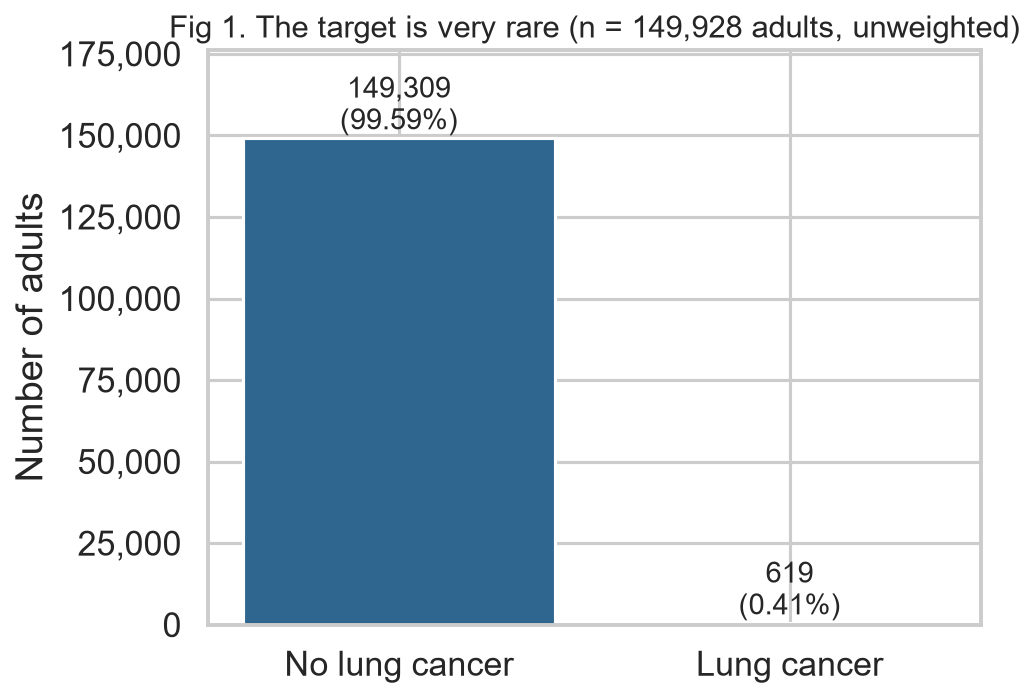
\includegraphics[width=0.55\textwidth]{fig01_class_balance}
\caption{Class balance of the target. Only \nCases of \nAdults adults (\sampleRate\%) report a lung-cancer diagnosis; the population rate after NHIS survey weighting is 0.31\%.}\label{fig:balance}
\end{figure}

The imbalance is extreme (Fig.~\ref{fig:balance}): a model that always answers ``no'' would be 99.59\% accurate while finding no one. This single number drove our choice of effect sizes (odds ratios rather than accuracy-like measures), of a stratified train/test split, and of the metrics planned for the modelling phase.

\subsection{Who is in the data: a detailed profile of the study population}\label{sec:profile}

Before testing anything, we describe exactly who the \nAdults adults are and where the \nCases cases sit. Tables~\ref{tab:prof-demo}--\ref{tab:prof-conditions} give, for every category of every variable, the number of adults, their share of the sample and of the US adult population (survey-weighted), the number of adults with and without a lung-cancer history, the lung-cancer rate in the sample and in the population, and the mean age of the group. ``Unknown'' rows are people who did not give a usable answer; we keep them so that every block adds up to \nAdults adults and \nCases cases (shares therefore differ slightly from Fig.~\ref{fig:categorical}, which uses known answers only). All numbers come from \file{reports/tables/population_profile.csv}, produced by \file{scripts/supplementary_analysis.py}.

Two reading rules apply throughout. First, the sample rate is what we observe among the people interviewed, while the weighted rate estimates the rate among all US adults: NHIS interviews some groups more than others (for example, 31.1\% of the adults with a known age are 65 or older, against 21.9\% of the population), and the survey weights correct for this. Second, raw counts of cases depend on group size: 507 of the \nCases cases are White adults simply because White adults are 67.5\% of the sample, so groups are compared through their rates, never through their counts.

\subsubsection{Demographics: sex, age and race/ethnicity}\label{sec:demo}

\begin{table}[htbp]
\centering\footnotesize
\caption{Demographic profile of the \nAdults adults: adults, share of the sample and of the US adult population (weighted, wtd), adults with and without a lung-cancer history, lung-cancer rate and mean age, by sex, age group and race/ethnicity. AIAN = American Indian or Alaska Native.}\label{tab:prof-demo}
\begin{tabular*}{\textwidth}{@{\extracolsep{\fill}}lrrrrrrrr}
\toprule
Group & Adults & \makecell[b]{\% of\\{}sample} & \makecell[b]{\% of US\\{}adults (wtd)} & \makecell[b]{Lung\\{}cancer} & \makecell[b]{No lung\\{}cancer} & \makecell[b]{Rate\\{}(sample)} & \makecell[b]{Rate\\{}(wtd)} & \makecell[b]{Mean\\{}age} \\
\midrule
\textbf{Sex} &  &  &  &  &  &  &  &  \\
\quad Female & 81,360 & 54.3 & 51.5 & 354 & 81,006 & 0.44\% & 0.32\% & 53.6 \\
\quad Male & 68,552 & 45.7 & 48.5 & 265 & 68,287 & 0.39\% & 0.30\% & 51.9 \\
\quad Unknown & 16 & 0.0 & 0.0 & 0 & 16 & 0.00\% & 0.00\% & 37.6 \\
\midrule
\textbf{Age group (years)} &  &  &  &  &  &  &  &  \\
\quad 18--44 & 54,481 & 36.3 & 45.8 & 13 & 54,468 & 0.02\% & 0.02\% & 32.4 \\
\quad 45--54 & 21,574 & 14.4 & 15.7 & 21 & 21,553 & 0.10\% & 0.08\% & 49.6 \\
\quad 55--64 & 27,020 & 18.0 & 16.5 & 113 & 26,907 & 0.42\% & 0.45\% & 59.7 \\
\quad 65--74 & 26,445 & 17.6 & 13.0 & 222 & 26,223 & 0.84\% & 0.81\% & 69.3 \\
\quad 75+ & 20,055 & 13.4 & 8.9 & 249 & 19,806 & 1.24\% & 1.25\% & 80.5 \\
\quad Unknown & 353 & 0.2 & 0.2 & 1 & 352 & 0.28\% & 0.11\% & -- \\
\midrule
\textbf{Race / ethnicity} &  &  &  &  &  &  &  &  \\
\quad White & 101,181 & 67.5 & 62.5 & 507 & 100,674 & 0.50\% & 0.39\% & 55.3 \\
\quad Hispanic & 20,411 & 13.6 & 17.0 & 27 & 20,384 & 0.13\% & 0.10\% & 45.0 \\
\quad Black & 16,138 & 10.8 & 11.8 & 55 & 16,083 & 0.34\% & 0.22\% & 51.3 \\
\quad Asian & 8,453 & 5.6 & 6.0 & 16 & 8,437 & 0.19\% & 0.22\% & 46.9 \\
\quad AIAN & 962 & 0.6 & 0.7 & 8 & 954 & 0.83\% & 0.60\% & 50.5 \\
\quad AIAN and other & 1,114 & 0.7 & 0.7 & 5 & 1,109 & 0.45\% & 0.43\% & 52.2 \\
\quad Other or multiple & 1,669 & 1.1 & 1.3 & 1 & 1,668 & 0.06\% & 0.02\% & 41.2 \\
\bottomrule
\end{tabular*}

\end{table}

\begin{itemize}
  \item \textbf{Sex.} The sample has 81,360 women (54.3\%) and 68,552 men (45.7\%); after weighting the split is 51.5\% / 48.5\%. More cases are women (354, against 265 men), but women are also more numerous and slightly older (mean age 53.6 vs 51.9 years), and the weighted rates are almost equal (0.32\% vs 0.30\%). Section~\ref{sec:sociodemo} confirms that sex is not associated with lung cancer.
  \item \textbf{Age.} Adults aged 18--44 are the largest group (36.3\% of the sample, 45.8\% of the population) but include only 13 cases (0.02\%). From there the rate climbs steadily: 0.10\% at 45--54, 0.42\% at 55--64, 0.84\% at 65--74 and 1.24\% at 75+. The 46,500 adults aged 65 or older (31.1\% of those with a known age) hold 471 of the \nCases cases (76.1\%; 76.2\% of the 618 cases with a known age, as in Table~\ref{tab:cases}).
  \item \textbf{Race and ethnicity.} NHIS records Hispanic origin and race in one variable; it is the only measure of cultural background in our variable set. The sample has 101,181 White adults (507 with and 100,674 without a lung-cancer history), 20,411 Hispanic adults (27 with, 20,384 without), 16,138 Black adults (55 with, 16,083 without), 8,453 Asian adults (16 with, 8,437 without), and three small groups -- AIAN (American Indian or Alaska Native, 962 adults, 8 cases), AIAN and another group (1,114 adults, 5 cases) and other or multiple races (1,669 adults, 1 case). The weighted rate is highest among White adults (0.39\%) and lowest among Hispanic adults (0.10\%). The three small groups total only 14 cases, so their rates are unstable and they are merged for testing (\S\ref{sec:sociodemo}).
\end{itemize}

\textbf{Why the groups differ.} Table~\ref{tab:group-profile} looks inside each sex and race/ethnicity group. White adults are the oldest group (mean age 55.3, 36.5\% aged 65+) and the most likely, after the AIAN groups, to have ever smoked (42.7\%); Hispanic adults are among the youngest (mean 45.0, 15.5\% aged 65+) and smoke much less (25.0\% ever-smokers). Asian adults have the lowest smoking prevalence (18.3\%). Age and smoking -- the two strongest risk factors in this project -- therefore explain a large part of the raw differences between race/ethnicity groups, which is why we do not interpret those differences as an effect of race itself. Men smoke more than women (43.4\% vs 32.9\% ever-smokers), yet women are older on average and report COPD slightly more often (6.2\% vs 5.0\%), which is consistent with the near-equal rates by sex.

\begin{table}[htbp]
\centering\footnotesize
\caption{Inside each sex and race/ethnicity group: age, sex, smoking and COPD, which explain much of the difference in lung-cancer rates (percentages among adults with a known answer; rate weighted). Source: \texttt{group\_profile.csv}.}\label{tab:group-profile}
\begin{tabular*}{\textwidth}{@{\extracolsep{\fill}}lrrrrrrrrr}
\toprule
Group & Adults & Cases & \makecell[b]{Mean\\{}age} & \makecell[b]{Median\\{}age} & \makecell[b]{\% aged\\{}65+} & \makecell[b]{\%\\{}women} & \makecell[b]{\% ever\\{}smoked} & \makecell[b]{\%\\{}COPD} & \makecell[b]{Rate\\{}(wtd)} \\
\midrule
\textbf{Sex} &  &  &  &  &  &  &  &  &  \\
\quad Female & 81,360 & 354 & 53.6 & 55 & 32.9 & -- & 32.9 & 6.2 & 0.32\% \\
\quad Male & 68,552 & 265 & 51.9 & 53 & 29.0 & -- & 43.4 & 5.0 & 0.30\% \\
\midrule
\textbf{Race / ethnicity} &  &  &  &  &  &  &  &  &  \\
\quad White & 101,181 & 507 & 55.3 & 58 & 36.5 & 53.5 & 42.7 & 6.7 & 0.39\% \\
\quad Hispanic & 20,411 & 27 & 45.0 & 43 & 15.5 & 54.3 & 25.0 & 2.4 & 0.10\% \\
\quad Black & 16,138 & 55 & 51.3 & 52 & 26.2 & 59.0 & 30.9 & 5.2 & 0.22\% \\
\quad Asian & 8,453 & 16 & 46.9 & 44 & 18.5 & 54.2 & 18.3 & 1.0 & 0.22\% \\
\quad AIAN & 962 & 8 & 50.5 & 51 & 23.8 & 57.1 & 50.4 & 10.5 & 0.60\% \\
\quad AIAN and other & 1,114 & 5 & 52.2 & 53.5 & 28.6 & 57.5 & 50.6 & 11.6 & 0.43\% \\
\quad Other or multiple & 1,669 & 1 & 41.2 & 38 & 11.7 & 53.9 & 32.5 & 2.4 & 0.02\% \\
\bottomrule
\end{tabular*}

\end{table}

\subsubsection{Socio-economic position, region and survey year}\label{sec:socio}

\begin{table}[htbp]
\centering\footnotesize
\caption{Socio-economic, geographic and yearly profile (same columns as Table~\ref{tab:prof-demo}). Income is family income divided by the poverty line.}\label{tab:prof-socio}
\begin{tabular*}{\textwidth}{@{\extracolsep{\fill}}lrrrrrrrr}
\toprule
Group & Adults & \makecell[b]{\% of\\{}sample} & \makecell[b]{\% of US\\{}adults (wtd)} & \makecell[b]{Lung\\{}cancer} & \makecell[b]{No lung\\{}cancer} & \makecell[b]{Rate\\{}(sample)} & \makecell[b]{Rate\\{}(wtd)} & \makecell[b]{Mean\\{}age} \\
\midrule
\textbf{Education} &  &  &  &  &  &  &  &  \\
\quad Less than high school & 12,809 & 8.5 & 10.9 & 86 & 12,723 & 0.67\% & 0.49\% & 56.8 \\
\quad High school / GED & 37,368 & 24.9 & 27.5 & 219 & 37,149 & 0.59\% & 0.40\% & 53.7 \\
\quad Some college & 42,452 & 28.3 & 29.2 & 195 & 42,257 & 0.46\% & 0.32\% & 52.4 \\
\quad Bachelor & 34,364 & 22.9 & 19.8 & 64 & 34,300 & 0.19\% & 0.15\% & 50.3 \\
\quad Graduate & 22,175 & 14.8 & 11.9 & 48 & 22,127 & 0.22\% & 0.16\% & 53.5 \\
\quad Unknown & 760 & 0.5 & 0.7 & 7 & 753 & 0.92\% & 0.59\% & 54.5 \\
\midrule
\textbf{Family income vs poverty line} &  &  &  &  &  &  &  &  \\
\quad Below poverty ($<$1) & 15,119 & 10.1 & 10.2 & 95 & 15,024 & 0.63\% & 0.46\% & 50.5 \\
\quad Low (1--2) & 26,307 & 17.5 & 18.0 & 164 & 26,143 & 0.62\% & 0.43\% & 54.2 \\
\quad Middle (2--4) & 44,165 & 29.5 & 30.1 & 187 & 43,978 & 0.42\% & 0.32\% & 53.2 \\
\quad High (4+) & 64,337 & 42.9 & 41.7 & 173 & 64,164 & 0.27\% & 0.21\% & 52.5 \\
\midrule
\textbf{Census region} &  &  &  &  &  &  &  &  \\
\quad Northeast & 24,963 & 16.6 & 17.6 & 117 & 24,846 & 0.47\% & 0.37\% & 53.8 \\
\quad Midwest & 33,049 & 22.0 & 20.8 & 174 & 32,875 & 0.53\% & 0.42\% & 53.2 \\
\quad South & 54,341 & 36.2 & 38.0 & 229 & 54,112 & 0.42\% & 0.29\% & 52.9 \\
\quad West & 37,575 & 25.1 & 23.6 & 99 & 37,476 & 0.26\% & 0.20\% & 51.7 \\
\midrule
\textbf{Survey year} &  &  &  &  &  &  &  &  \\
\quad 2019 & 31,925 & 21.3 & 19.7 & 112 & 31,813 & 0.35\% & 0.28\% & 52.0 \\
\quad 2020 & 31,513 & 21.0 & 19.9 & 131 & 31,382 & 0.42\% & 0.31\% & 53.5 \\
\quad 2021 & 29,430 & 19.6 & 19.9 & 115 & 29,315 & 0.39\% & 0.28\% & 52.5 \\
\quad 2022 & 27,594 & 18.4 & 20.1 & 116 & 27,478 & 0.42\% & 0.34\% & 52.9 \\
\quad 2023 & 29,466 & 19.7 & 20.3 & 145 & 29,321 & 0.49\% & 0.34\% & 53.2 \\
\bottomrule
\end{tabular*}

\end{table}

\begin{itemize}
  \item \textbf{Education.} The largest groups are ``some college'' (42,452 adults, 28.3\%) and high school / GED (37,368, 24.9\%; Table~\ref{tab:prof-socio}). The rate falls from 0.67\% (sample) among adults without a high-school diploma to 0.19\% among bachelor's graduates; weighted, from 0.49\% to 0.15\%.
  \item \textbf{Income.} 42.9\% of adults have a family income at least four times the poverty line and 10.1\% live below it. The rate halves from below-poverty (0.46\% weighted) to high income (0.21\%).
  \item \textbf{Region.} The South is the largest region (54,341 adults, 36.2\%), followed by the West (25.1\%), the Midwest (22.0\%) and the Northeast (16.6\%). The weighted rate is highest in the Midwest (0.42\%) and lowest in the West (0.20\%); the matching sample rates are 0.53\% and 0.26\%. The West is also the youngest region (mean age 51.7).
  \item \textbf{Survey year.} Each year contributes 27,594--31,925 adults and 112--145 cases. The rate drifts upward from 0.35\% in 2019 to 0.49\% in 2023 (weighted, 0.28\% to 0.34\%), but the difference between years is not statistically significant ($\chi^2(4) = 7.9$, $p = 0.096$; \file{rate_by_year.csv}). This matters because 2019 was the first year of the redesigned NHIS questionnaire and 2020 collection was disrupted by COVID-19 (largely telephone interviews); because the years do not differ significantly, pooling them is reasonable, and we keep year in the data so the modelling phase can check it again.
\end{itemize}

\subsubsection{Smoking, body weight, self-rated health and chronic conditions}\label{sec:smokingprofile}

\begin{table}[htbp]
\centering\footnotesize
\caption{Smoking, e-cigarette use, body weight and self-rated health (same columns as Table~\ref{tab:prof-demo}).}\label{tab:prof-smoking}
\begin{tabular*}{\textwidth}{@{\extracolsep{\fill}}lrrrrrrrr}
\toprule
Group & Adults & \makecell[b]{\% of\\{}sample} & \makecell[b]{\% of US\\{}adults (wtd)} & \makecell[b]{Lung\\{}cancer} & \makecell[b]{No lung\\{}cancer} & \makecell[b]{Rate\\{}(sample)} & \makecell[b]{Rate\\{}(wtd)} & \makecell[b]{Mean\\{}age} \\
\midrule
\textbf{Cigarette smoking} &  &  &  &  &  &  &  &  \\
\quad Never & 90,937 & 60.7 & 63.5 & 107 & 90,830 & 0.12\% & 0.08\% & 50.3 \\
\quad Former & 37,452 & 25.0 & 22.0 & 367 & 37,085 & 0.98\% & 0.81\% & 59.7 \\
\quad Current & 17,586 & 11.7 & 11.7 & 127 & 17,459 & 0.72\% & 0.60\% & 51.1 \\
\quad Unknown & 3,953 & 2.6 & 2.8 & 18 & 3,935 & 0.46\% & 0.32\% & 52.9 \\
\midrule
\textbf{Ever used an e-cigarette} &  &  &  &  &  &  &  &  \\
\quad No & 122,606 & 81.8 & 79.4 & 497 & 122,109 & 0.41\% & 0.31\% & 55.1 \\
\quad Yes & 23,470 & 15.7 & 17.8 & 105 & 23,365 & 0.45\% & 0.29\% & 41.0 \\
\quad Unknown & 3,852 & 2.6 & 2.8 & 17 & 3,835 & 0.44\% & 0.32\% & 52.7 \\
\midrule
\textbf{BMI category} &  &  &  &  &  &  &  &  \\
\quad Underweight & 2,324 & 1.6 & 1.6 & 33 & 2,291 & 1.42\% & 1.14\% & 51.7 \\
\quad Healthy & 46,153 & 30.8 & 30.7 & 221 & 45,932 & 0.48\% & 0.35\% & 51.6 \\
\quad Overweight & 50,466 & 33.7 & 33.2 & 187 & 50,279 & 0.37\% & 0.29\% & 54.2 \\
\quad Obese & 47,471 & 31.7 & 32.2 & 165 & 47,306 & 0.35\% & 0.24\% & 52.4 \\
\quad Unknown & 3,514 & 2.3 & 2.3 & 13 & 3,501 & 0.37\% & 0.28\% & 54.6 \\
\midrule
\textbf{Self-rated general health} &  &  &  &  &  &  &  &  \\
\quad Excellent & 32,824 & 21.9 & 23.4 & 18 & 32,806 & 0.05\% & 0.03\% & 46.5 \\
\quad Very good & 51,131 & 34.1 & 33.9 & 73 & 51,058 & 0.14\% & 0.10\% & 51.1 \\
\quad Good & 42,973 & 28.7 & 28.3 & 173 & 42,800 & 0.40\% & 0.28\% & 55.4 \\
\quad Fair & 17,483 & 11.7 & 11.1 & 206 & 17,277 & 1.18\% & 0.96\% & 59.8 \\
\quad Poor & 5,457 & 3.6 & 3.3 & 149 & 5,308 & 2.73\% & 2.47\% & 63.4 \\
\quad Unknown & 60 & 0.0 & 0.0 & 0 & 60 & 0.00\% & 0.00\% & 61.5 \\
\bottomrule
\end{tabular*}

\end{table}

\begin{table}[htbp]
\centering\footnotesize
\caption{Chronic conditions (ever told by a doctor) and the number of the five conditions (same columns as Table~\ref{tab:prof-demo}).}\label{tab:prof-conditions}
\begin{tabular*}{\textwidth}{@{\extracolsep{\fill}}lrrrrrrrr}
\toprule
Group & Adults & \makecell[b]{\% of\\{}sample} & \makecell[b]{\% of US\\{}adults (wtd)} & \makecell[b]{Lung\\{}cancer} & \makecell[b]{No lung\\{}cancer} & \makecell[b]{Rate\\{}(sample)} & \makecell[b]{Rate\\{}(wtd)} & \makecell[b]{Mean\\{}age} \\
\midrule
\textbf{COPD} &  &  &  &  &  &  &  &  \\
\quad No & 141,386 & 94.3 & 95.3 & 330 & 141,056 & 0.23\% & 0.17\% & 52.0 \\
\quad Yes & 8,440 & 5.6 & 4.6 & 288 & 8,152 & 3.41\% & 3.13\% & 65.4 \\
\quad Unknown & 102 & 0.1 & 0.1 & 1 & 101 & 0.98\% & 0.32\% & 64.8 \\
\midrule
\textbf{Heart disease} &  &  &  &  &  &  &  &  \\
\quad No & 140,524 & 93.7 & 95.0 & 475 & 140,049 & 0.34\% & 0.25\% & 51.6 \\
\quad Yes & 9,073 & 6.1 & 4.8 & 139 & 8,934 & 1.53\% & 1.52\% & 70.7 \\
\quad Unknown & 331 & 0.2 & 0.2 & 5 & 326 & 1.51\% & 1.34\% & 69.9 \\
\midrule
\textbf{Hypertension} &  &  &  &  &  &  &  &  \\
\quad No & 94,990 & 63.4 & 68.2 & 215 & 94,775 & 0.23\% & 0.16\% & 46.7 \\
\quad Yes & 54,776 & 36.5 & 31.7 & 404 & 54,372 & 0.74\% & 0.63\% & 63.3 \\
\quad Unknown & 162 & 0.1 & 0.1 & 0 & 162 & 0.00\% & 0.00\% & 58.7 \\
\midrule
\textbf{Diabetes} &  &  &  &  &  &  &  &  \\
\quad No & 133,796 & 89.2 & 90.4 & 488 & 133,308 & 0.36\% & 0.26\% & 51.4 \\
\quad Yes & 16,064 & 10.7 & 9.5 & 131 & 15,933 & 0.82\% & 0.74\% & 64.5 \\
\quad Unknown & 68 & 0.0 & 0.0 & 0 & 68 & 0.00\% & 0.00\% & 59.7 \\
\midrule
\textbf{Asthma} &  &  &  &  &  &  &  &  \\
\quad No & 129,025 & 86.1 & 85.8 & 502 & 128,523 & 0.39\% & 0.29\% & 53.2 \\
\quad Yes & 20,839 & 13.9 & 14.2 & 116 & 20,723 & 0.56\% & 0.41\% & 50.2 \\
\quad Unknown & 64 & 0.0 & 0.0 & 1 & 63 & 1.56\% & 2.55\% & 57.4 \\
\midrule
\textbf{Number of the 5 conditions} &  &  &  &  &  &  &  &  \\
\quad 0 & 76,217 & 50.8 & 55.2 & 87 & 76,130 & 0.11\% & 0.08\% & 45.9 \\
\quad 1 & 47,541 & 31.7 & 29.9 & 203 & 47,338 & 0.43\% & 0.33\% & 57.0 \\
\quad 2 & 18,719 & 12.5 & 10.8 & 166 & 18,553 & 0.89\% & 0.74\% & 64.2 \\
\quad 3 & 5,808 & 3.9 & 3.2 & 118 & 5,690 & 2.03\% & 2.05\% & 67.1 \\
\quad 4 & 1,426 & 1.0 & 0.8 & 36 & 1,390 & 2.52\% & 2.24\% & 68.0 \\
\quad 5 & 217 & 0.1 & 0.1 & 9 & 208 & 4.15\% & 3.79\% & 66.7 \\
\bottomrule
\end{tabular*}

\end{table}

\begin{itemize}
  \item \textbf{Smoking.} 90,937 adults have never smoked (60.7\% of all adults, 62.3\% of those who answered), 37,452 are former and 17,586 current smokers; 3,953 did not answer. Former smokers have the highest rate (0.98\% sample, 0.81\% weighted) and are much older (mean age \formerSmokerAge, against 51.1 for current and 50.3 for never-smokers), a first hint of the reverse causation discussed in \S\ref{sec:rq1}.
  \item \textbf{E-cigarettes.} 23,470 adults (15.7\%) have ever used one. They are much younger (mean age 41.0 vs 55.1), which is why their crude rate (0.29\% weighted) is close to that of non-users (0.31\%).
  \item \textbf{Body weight and self-rated health.} Underweight adults are only 1.6\% of the sample but have the highest rate (1.42\%, 33 cases). Self-rated health shows the steepest gradient in the whole dataset: 0.05\% for ``excellent'' up to 2.73\% for ``poor'' (sample rates), with 149 cases among the 5,457 adults in poor health.
  \item \textbf{Chronic conditions.} 8,440 adults (5.6\%) report COPD, and 288 of them have a lung-cancer history -- 46.5\% of all cases, at a rate of 3.41\%, fifteen times the 0.23\% of adults without COPD. About half of adults (50.8\%) have none of the five conditions; the rate then rises with every additional condition, from 0.11\% with none to 4.15\% with all five.
\end{itemize}

\subsubsection{Adults with and without a lung-cancer history, side by side}\label{sec:sidebyside}

Table~\ref{tab:cases} summarises the same information from the other direction: what the \nCases cases look like compared with the 149,309 other adults. Cases are about 18.5 years older on average (71.2 vs 52.7), are more than twice as likely to have ever smoked (82.2\% vs 37.5\%), are eight times as likely to report COPD (46.6\% vs 5.5\%) and almost four times as likely to rate their health as fair or poor (57.4\% vs 15.1\%). They are more often White (81.9\% vs 67.4\%) and less often Hispanic (4.4\% vs 13.7\%) -- a difference that the age and smoking profiles of Table~\ref{tab:group-profile} largely explain -- and the share of women is similar (57.2\% vs 54.3\%).

\begin{table}[htbp]
\centering\small
\caption{Characteristics of adults with and without a lung-cancer history (unweighted; percentages among adults with a known answer). Source: \texttt{cases\_vs\_noncases.csv}.}\label{tab:cases}
\begin{tabular}{lrr}
\toprule
Characteristic & Lung cancer & No lung cancer \\
\midrule
Adults & 619 & 149,309 \\
Age, mean (years) & 71.2 & 52.7 \\
Age, standard deviation (years) & 10.2 & 18.3 \\
Age, median (years) & 72.0 & 54.0 \\
Age, interquartile range (years) & 65--79 & 37--68 \\
Aged 65 or older & 76.2\% & 30.9\% \\
Female & 57.2\% & 54.3\% \\
Race/ethnicity -- White & 81.9\% & 67.4\% \\
Race/ethnicity -- Hispanic & 4.4\% & 13.7\% \\
Race/ethnicity -- Black & 8.9\% & 10.8\% \\
Race/ethnicity -- Asian & 2.6\% & 5.7\% \\
Race/ethnicity -- AIAN / other / multiple & 2.3\% & 2.5\% \\
Ever smoked (former or current) & 82.2\% & 37.5\% \\
Current smoker & 21.1\% & 12.0\% \\
Ever used an e-cigarette & 17.4\% & 16.1\% \\
COPD & 46.6\% & 5.5\% \\
Heart disease & 22.6\% & 6.0\% \\
Hypertension & 65.3\% & 36.5\% \\
Diabetes & 21.2\% & 10.7\% \\
Asthma & 18.8\% & 13.9\% \\
Comorbidity count, mean & 1.7 & 0.7 \\
Fair or poor self-rated health & 57.4\% & 15.1\% \\
Underweight & 5.4\% & 1.6\% \\
Obese & 27.2\% & 32.4\% \\
Less than high school & 14.1\% & 8.6\% \\
Bachelor or graduate degree & 18.3\% & 38.0\% \\
Family income below the poverty line & 15.3\% & 10.1\% \\
Region -- Northeast & 18.9\% & 16.6\% \\
Region -- Midwest & 28.1\% & 22.0\% \\
Region -- South & 37.0\% & 36.2\% \\
Region -- West & 16.0\% & 25.1\% \\
\bottomrule
\end{tabular}

\end{table}

\subsection{Initial data-quality issues and limitations}\label{sec:quality}

\begin{itemize}
  \item \textbf{Severe imbalance:} \nCases cases out of \nAdults adults (\sampleRate\%).
  \item \textbf{Hidden missing values:} NHIS stores ``refused / not ascertained / don't know'' as numbers (7, 8, 9 or 97, 98, 99) that look like real values; 4,424 such codes sat in just four key columns.
  \item \textbf{A renamed column:} education is \file{EDUC_A} in 2019--2020 but \file{EDUCP_A} from 2021 (same codes), and code 11 (doctorate) exists only in 2019--2020.
  \item \textbf{Self-reported, lifetime answers:} someone diagnosed years ago may have quit smoking or lost weight since, so current habits can be a result of the cancer (reverse causation).
  \item \textbf{No smoking dose:} NHIS has no pack-years or quit dates, so we can only approximate the official screening group.
  \item \textbf{Survey design:} NHIS is not a simple random sample. It over-samples some groups -- the sample is older than the population (31.1\% aged 65+ vs 21.9\% after weighting) -- so raw rates (\sampleRate\%) differ from population rates (0.31\%).
  \item \textbf{Year comparability:} the 2019 questionnaire redesign and the 2020 pandemic disruption could affect comparability between years; the year-to-year differences in the case rate are not significant ($p = 0.096$).
  \item \textbf{Coarse regional data:} each regional variable has only 20 distinct values (4 regions $\times$ 5 years), so it is ecological context, not personal exposure.
  \item \textbf{Possible repeats across years:} people cannot be linked between survey years, so a few adults may appear in two different years.
\end{itemize}

\subsection{The dataset we rejected}\label{sec:rejected}

We started the project with a 22,457-row file (\file{lung_cancer_combined_22457.csv}, no documented origin) that has the same columns as the well-known 309-person Kaggle lung-cancer survey~\cite{kaggle}. Before using it we audited it the way we would review an unknown dependency, and it failed review (Table~\ref{tab:audit}). The decisive evidence is the row order and the lineage; duplicates and label conflicts alone would be weak evidence, because a file with about fifteen low-cardinality columns produces repeated answer patterns naturally.

\begin{table}[htbp]
\centering\small
\caption{Integrity audit of the supplied file (all numbers recomputed from the file), strongest evidence first.}\label{tab:audit}
\begin{tabularx}{\textwidth}{@{}>{\raggedright\arraybackslash}p{2.6cm} >{\raggedright\arraybackslash}X >{\raggedright\arraybackslash}p{4.6cm}@{}}
\toprule
Check & Finding & Why it matters \\
\midrule
Row order & the first 1,455 rows are all negative; the first positive label appears at row 1,456 & row position (and \texttt{patient\_id}) predicts the label -- a leakage path \\
Lineage & only 1,438 rows (6.4\%) match a row of the public 309-person survey (252 of its patterns, one repeated 59 times; labels agree in 99.4\% of matches); the other 21,019 rows match no public source & most of the file has no traceable origin \\
Signal after deduplication & no feature is associated with the label (all Cram\'er's $V < 0.02$) & the apparent signal came from the duplicates and the ordered block \\
Exact duplicates & 2,573 rows repeat another row exactly & the same answers counted many times inflate every statistic \\
Label conflicts & 133 identical answer patterns carry both labels (315 rows) & the label is not a clean function of the answers \\
\bottomrule
\end{tabularx}
\end{table}

This pattern is statistically consistent with resampling or programmatic generation; it is not proof that the data are synthetic. We replaced the file with NHIS and kept it in \file{data/raw/other/} so the decision stays auditable. The lineage numbers were recomputed against an identical public copy of the Kaggle survey~\cite{kaggle}.

\section{Preprocessing Methodology}\label{sec:prep}

We lost only 292 of \nRawRows rows (0.19\%), all of them people whose cancer answer was unknown, and ended with 0 missing values in the model-ready file.

\subsection{A logged, reproducible pipeline}\label{sec:pipeline}

We built the cleaning as a pipeline in Python (pandas, SciPy~\cite{scipy}, scikit-learn~\cite{sklearn}, statsmodels~\cite{statsmodels}) rather than as notebook cells run by hand:
\begin{itemize}
  \item each step lives in a script -- \file{build_regional_data.py} for the three regional sources and \file{build_clean_dataset.py} for NHIS;
  \item each step records its effect (rows, columns, missing cells) in \file{data/clean/before_after_summary.csv} and explains itself in \file{data/clean/cleaning_report.txt};
  \item the whole project runs from one entry point, \texttt{python run\_all.py} (Table~\ref{tab:pipeline-steps}), with every random step seeded (42).
\end{itemize}
That made every decision below (Table~\ref{tab:problems}) easy to review and easy to undo, and it guarantees that the numbers in this report are the numbers the code produces.

\subsection{Problems found and treatments applied}\label{sec:problems}

Table~\ref{tab:problems} lists every data-quality problem we found, what we did about it, why, and its measured effect.

\begin{table}[htbp]
\centering\footnotesize
\caption{Data-quality problems, the treatment applied, the reason, and its measured effect.}\label{tab:problems}
\begin{tabularx}{\textwidth}{@{}>{\raggedright\arraybackslash}p{3.5cm} >{\raggedright\arraybackslash}X >{\raggedright\arraybackslash}p{3.7cm} >{\raggedright\arraybackslash}p{3.0cm}@{}}
\toprule
Problem found & What we did & Why & Effect \\
\midrule
Five yearly files; education renamed \texttt{EDUCP\_A} from 2021; doctorate coded 11 only in 2019--2020 & stacked the years, mapped both names to one column, mapped code 11 to ``Graduate'' & same codes every year, so one schema works & \nRawRows rows $\times$ 20 columns \\
Possible duplicate people & built \texttt{person\_id} = year + household number and checked for repeats & NHIS interviews one adult per household per year, so the key is unique by design; the check guards against a stacking error rather than finding real duplicates & 0 duplicates found \\
No ready-made target; \texttt{LUNGCAN\_A} only asked to people who had any cancer & 0 = no cancer or another cancer; 1 = lung cancer; refused / don't know $\rightarrow$ row removed & ``don't know'' is not ``no'', and we never impute a target & 292 rows removed; \nAdults kept, \nCases cases \\
Missing values hidden as numbers (7/8/9, 97/98/99) & recoded every column to readable labels; those codes $\rightarrow$ missing & otherwise a model would read 97 as a real value & 4,424 hidden codes in 4 key columns became missing \\
Inconsistent categories (e.g.\ smoking codes 1, 2, 5 all mean ``current'') & merged into one label per meaning (Current / Former / Never) & one category per real-world meaning & 3 clean smoking groups \\
Regional sources at a finer level (monitor, state) than NHIS (region) & aggregated to 4 regions $\times$ 5 years, then a left join on region + year & public NHIS files only identify the region & 20 region-years; \nAdults rows before and after; 0 unmatched \\
Outliers & IQR rule on the 6 numeric columns plus a plausibility check of every flagged value (\S\ref{sec:outliers}) & remove what is impossible, not what is rare & 0 removed \\
Remaining missing values (at most 2.84\%, Fig.~\ref{fig:missing}) & categories $\rightarrow$ explicit Unknown; yes/no $\rightarrow$ 0 plus an \texttt{\_unknown} flag; age $\rightarrow$ training median (54) plus a flag & keep every row; no detectable link between missingness and the target (Table~\ref{tab:missing}) & 0 missing cells in the model-ready file \\
Features that are exact or near-exact combinations of several other features (\texttt{comorbidity\_count} = sum of 5 flags; complete one-hot groups summing to 1; region dummies vs the regional columns) -- invisible to a pairwise correlation filter & Rule 4 of feature selection: variance inflation factor (VIF) on training rows; dropped \texttt{comorbidity\_count} (kept for the EDA), one reference category per one-hot group and the region dummies & a linear model cannot be fitted with perfect multicollinearity, and its coefficients are unstable with near-perfect multicollinearity & VIF: \nInfVIF of \nFeaturesBefore features infinite $\rightarrow$ maximum \maxVIFshort (none above 10); \nFeaturesBefore $\rightarrow$ \nFeatures features \\
Leakage risk & never used \texttt{CANEV\_A} (``ever had any cancer'') as a feature; split before fitting anything & every case has \texttt{CANEV\_A} = yes, so it would reveal the answer & no feature derived from the target \\
\bottomrule
\end{tabularx}
\end{table}

\subsection{Missing values}\label{sec:missing}

Before filling any gap (Fig.~\ref{fig:missing}) we checked whether missingness itself carries information about the target. For every column with at least 1\% missing, we cross-tabulated ``value missing'' against lung cancer with a $\chi^2$ test (all expected counts $\geq 14.5$, so the test is valid).

\begin{figure}[htbp]
\centering
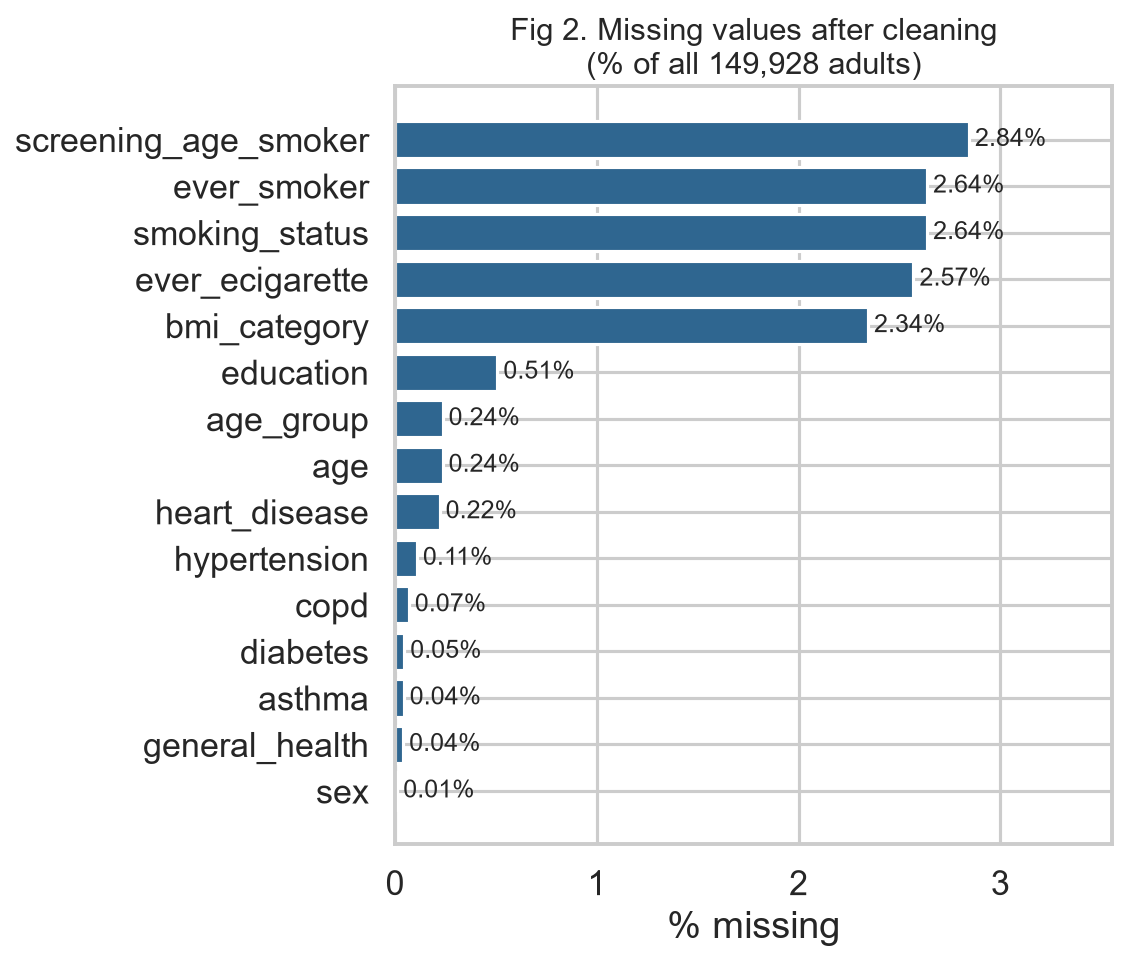
\includegraphics[width=0.55\textwidth]{fig02_missing_values}
\caption{Share of missing values per column after recoding the hidden ``unknown'' codes. The five smoking, e-cigarette and BMI columns are the only ones above 2.3\% (2.34--2.84\%); every other column is below 0.6\%.}\label{fig:missing}
\end{figure}

\begin{table}[htbp]
\centering\small
\caption{Is missingness related to lung cancer? $\chi^2$ tests of ``value missing (yes/no)'' $\times$ target.}\label{tab:missing}
\begin{tabular}{lrrrrrr}
\toprule
Column & \% missing & Rate if missing & Rate if present & $\chi^2$ & $p$ & Holm $p$ \\
\midrule
bmi\_category & 2.34 & 0.37\% & 0.41\% & 0.07 & 0.79 & 1.00 \\
ever\_ecigarette & 2.57 & 0.44\% & 0.41\% & 0.02 & 0.88 & 1.00 \\
smoking\_status / ever\_smoker & 2.64 & 0.46\% & 0.41\% & 0.09 & 0.77 & 1.00 \\
screening\_age\_smoker & 2.84 & 0.45\% & 0.41\% & 0.05 & 0.83 & 1.00 \\
\bottomrule
\end{tabular}

\end{table}

None of the differences is significant (all $p > 0.7$; Table~\ref{tab:missing}), so there is no detectable link between the gaps and lung cancer. We word this carefully: each missing group contains only about 14--18 expected cases, so the tests have little power, and they do not check whether missingness depends on other variables such as age or education. With at most 2.84\% missing per column, filling the gaps cannot move the main estimates much. We still keep an Unknown category or an \file{_unknown} flag wherever the gap is large enough to be informative, so a future model can learn from ``missing'' if it matters. Imputation values (the age median) are computed on training rows only (Section~\ref{sec:leakage}).

\subsection{Outliers}\label{sec:outliers}

The IQR rule flags values that are unusual, not values that are wrong (Fig.~\ref{fig:outliers}, Table~\ref{tab:outliers}). Removing the 7,451 adults with three or more chronic conditions would delete exactly the sick, older people among whom lung cancer is concentrated, and would bias every later estimate. Our rule was therefore to remove only impossible values; there were none.

\begin{figure}[htbp]
\centering
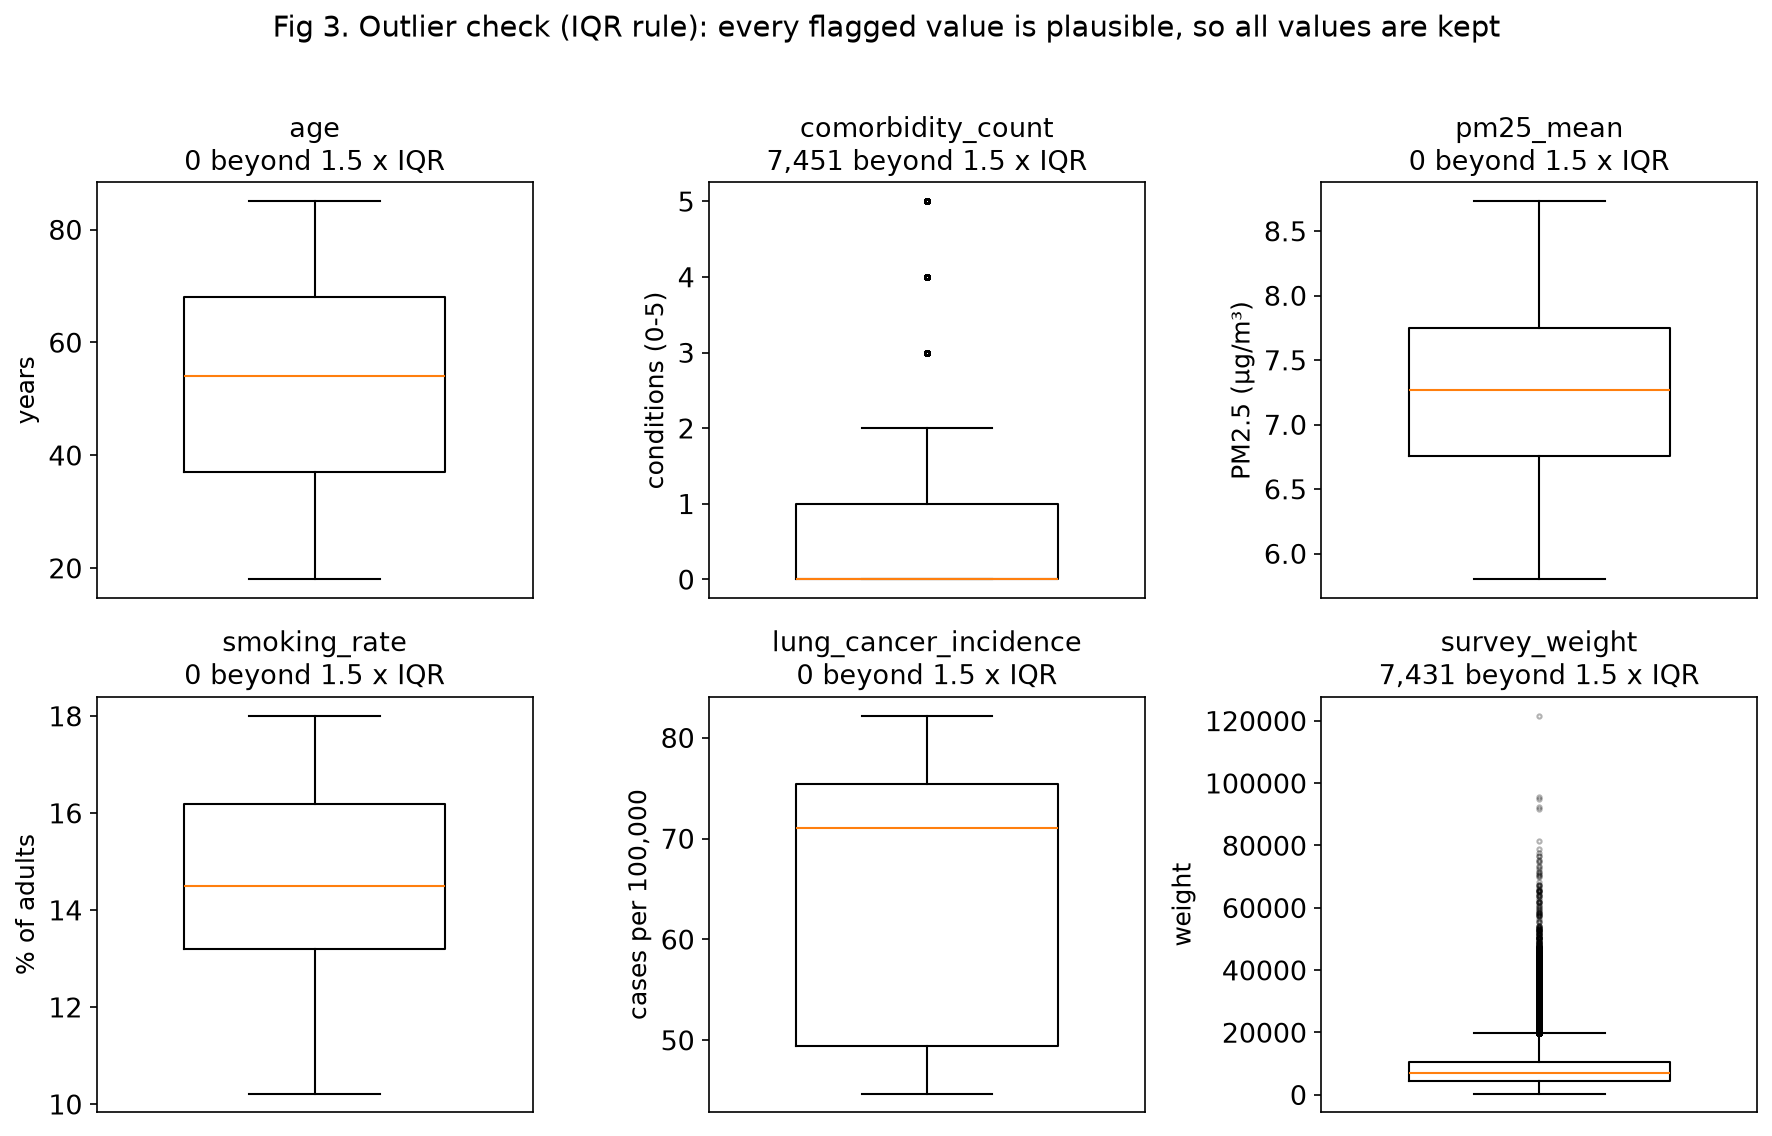
\includegraphics[width=0.85\textwidth]{fig03_outlier_boxplots}
\caption{Box plots of the six numeric columns with the number of values beyond $1.5 \times$ IQR. Every flagged value was checked for plausibility and kept.}\label{fig:outliers}
\end{figure}

\begin{table}[htbp]
\centering\small
\caption{Outlier check (IQR rule: below $Q_1 - 1.5 \times \mathrm{IQR}$ or above $Q_3 + 1.5 \times \mathrm{IQR}$) and the decision for each column.}\label{tab:outliers}
\begin{tabularx}{\textwidth}{l l r >{\raggedright\arraybackslash}X}
\toprule
Column & Bounds & Flagged & Decision and reason \\
\midrule
age & [$-$9.5, 114.5] & 0 (0\%) & keep -- every age 18-85 is a real adult; 85 means ``85 or older'' (NHIS top-code), not an error \\
comorbidity\_count & [$-$1.5, 2.5] & 7,451 (4.97\%) & keep -- a count from 0 to 5; high values are real people with several diseases \\
pm25\_mean & [5.3, 9.2] & 0 (0\%) & keep -- official EPA measurements; only 20 region-year values, none impossible \\
smoking\_rate & [8.7, 20.7] & 0 (0\%) & keep -- official CDC percentages between 0 and 100 \\
lung\_cancer\_incidence & [10.4, 114.4] & 0 (0\%) & keep -- official registry rates; differences between regions are real \\
survey\_weight & [$-$4883.8, 19849.6] & 7,431 (4.96\%) & keep -- NHIS design weight, used for population estimates only, not as a feature \\
\bottomrule
\end{tabularx}

\end{table}

\subsection{Integrating the regional sources}\label{sec:integration}

Each regional source needed its own cleaning before the three could be combined (\file{build_regional_data.py}; Table~\ref{tab:regional-cleaning}):

\begin{table}[htbp]
\centering\small
\caption{Cleaning and aggregation of the three regional sources.}\label{tab:regional-cleaning}
\begin{tabularx}{\textwidth}{@{}l >{\raggedright\arraybackslash}X >{\raggedright\arraybackslash}p{4.2cm}@{}}
\toprule
Source & Cleaning steps & Result \\
\midrule
EPA PM2.5 & kept the parameter ``PM2.5 -- Local Conditions'' and the official annual standard; kept ``No Events'' / ``Events Excluded'' rows (wildfire-type events removed); dropped values outside 0--100 \textmu g/m$^3$ and duplicate monitors; dropped 56 rows outside the 50 states + DC; averaged per state first (so states with many monitors do not dominate), then per region & 1,409--1,798 annual monitor values per year $\rightarrow$ 20 region-year means \\
BRFSS smoking & kept the ``current smoker = yes'' answer, years 2019--2023, values 0--100\%; dropped 21 territory / national rows; averaged per region & 1,644 rows $\rightarrow$ 251 state-years $\rightarrow$ 20 region-years \\
US Cancer Statistics & kept lung cancer, both sexes, all races, single years (multi-year rows dropped); suppressed counts treated as missing; region rate = sum of cases $\div$ sum of population $\times$ 100,000 & 23,796 rows $\rightarrow$ 255 state-years $\rightarrow$ 20 region-years \\
\bottomrule
\end{tabularx}
\end{table}

We mapped every state to its US Census region -- the same four regions NHIS uses -- and combined the three tables into one 20-row table (\file{data/clean/regional_context.csv}). No region-year was missing; the code would fill a missing year from the same region's nearest year and log it. The NHIS table was then left-joined on region + year with a many-to-one validation, and an assertion stops the pipeline if the join ever adds a row. Result: \nAdults rows before and after, 0 adults without a regional match.

Two aggregation choices are worth stating plainly because they are limitations: the registry rate is a crude rate (not age-adjusted), and states are averaged without population weights. Both are discussed in Section~\ref{sec:regional}.

\subsection{Effect of each step}\label{sec:effect}

Table~\ref{tab:before-after} follows the data through the pipeline. The column count changes for simple reasons: step 2 adds \file{person_id} ($20 \rightarrow 21$), step 3 adds the target (22), and step 4 replaces the raw NHIS columns with 19 readable ones (the helper columns \file{HHX}, \file{CANEV_A} and \file{LUNGCAN_A} are not carried forward). The missing cells fall sharply at step 4 because \file{LUNGCAN_A}, blank by design for everyone without cancer, is no longer carried; they rise again at step 5 only because the new columns inherit the gaps of the columns they are built from. The \nModelColumns columns of the model-ready file are the \nFeatures features plus \file{person_id}, \file{split}, \file{survey_weight} and the target.

\begin{table}[htbp]
\centering\footnotesize
\caption{Rows, columns and missing cells after each preprocessing step (\texttt{data/clean/before\_after\_summary.csv}).}\label{tab:before-after}
\begin{tabularx}{\textwidth}{>{\raggedright\arraybackslash}p{3.6cm} r r r >{\raggedright\arraybackslash}X}
\toprule
Step & Rows & Columns & Missing cells & What changed \\
\midrule
1. Load + stack 5 years & 150,220 & 20 & 131,400 & 5 yearly files stacked; 20 needed columns kept (LUNGCAN\_A is blank by design for people who never had cancer) \\
2. Remove duplicates & 150,220 & 21 & 131,400 & 0 duplicate person IDs removed \\
3. Build target & 149,928 & 22 & 131,217 & 292 rows with unknown answer removed \\
4. Recode codes $\rightarrow$ values & 149,928 & 19 & 13,235 & number codes turned into words; e.g. 4,424 ``unknown'' codes in 4 key columns $\rightarrow$ missing \\
5. New columns & 149,928 & 23 & 21,805 & added age\_group, ever\_smoker, screening\_age\_smoker, comorbidity\_count \\
5b. Join regional table & 149,928 & 26 & 21,805 & 3 columns added (pm25\_mean, smoking\_rate, lung\_cancer\_incidence); 0 rows added \\
5c. Outlier check & 149,928 & 26 & 21,805 & IQR check on 6 numeric columns; all values plausible $\rightarrow$ kept \\
6. Checks + save clean file & 149,928 & 26 & 21,805 & 0 duplicate IDs, ages 18-85, missing values listed \\
7. Encode + fill gaps (train only) & 149,928 & 71 & 0 & one-hot encoding, training-median filling, ``unknown'' flags $\rightarrow$ 0 missing \\
8. Feature selection & 149,928 & 42 & 0 & 29 redundant / near-constant / near-duplicate / linearly dependent features dropped; 38 kept (max VIF 7.5) \\
9. Scaling (train only) & 149,928 & 42 & 0 & 4 numeric columns standardised \\
\bottomrule
\end{tabularx}

\end{table}

\subsection{How we prevented data leakage}\label{sec:leakage}

We treated the test set like production data the model has never seen, following the leakage checklist of Kapoor and Narayanan~\cite{kapoor}:
\begin{itemize}
  \item The 80/20 split (stratified on the target, seed 42) happens before anything is learned from the data: \nTrain training rows and \nTest test rows, both with a \sampleRate\% case rate.
  \item The age median used for filling, the feature-selection rules and the VIF step, the scaler and the PCA are all computed on training rows only, then applied unchanged to the test rows.
  \item \file{CANEV_A} is never a candidate feature, \file{person_id} is an identifier only, and \file{survey_weight} is used for population estimates, never as a feature.
  \item A sanity check: after scaling, the training means are exactly 0 while the test means are slightly off ($-0.002$ for age, 0.006 for PM2.5, $-0.001$ for the regional smoking rate and 0.019 for registry incidence; Table~\ref{tab:scaler}). That is exactly what we expect if the scaler never saw the test rows, and \file{supplementary_analysis.py} turns it into an assertion: the saved scaler parameters must equal a refit on training rows only and must differ from a fit on all rows.
\end{itemize}

Descriptive statistics, the population profile and the hypothesis tests in Sections~\ref{sec:profile} and~\ref{sec:eda} use all adults, because they describe the population and fit nothing that a model reuses. Two design decisions were nevertheless informed by data on all rows, and we state them openly: merging the three smallest race groups for the $\chi^2$ test (a testing decision only; the model-ready file keeps all seven groups, with White as the reference), and the \file{screening_age_smoker} feature, which comes from the USPSTF rule~\cite{uspstf} and was only illustrated by Fig.~\ref{fig:agesmoking}. The one EDA step that ranks features (mutual information, \S\ref{sec:mi}) uses training rows only.

\section{Exploratory Data Analysis and Results}\label{sec:eda}

Age, smoking history and COPD separate people with and without lung cancer far more than any regional factor does. Fourteen of our eighteen tests stay significant after correction, but the effect sizes remind us that with 150,000 rows ``significant'' and ``important'' are not the same thing. For every test we followed the same checklist: state H$_0$, check the assumptions, run the test, report an effect size, and say what it means in plain words. Unless stated otherwise, $p$-values in the text are raw (before correction); Holm-adjusted values are always labelled ``Holm $p$''.

\subsection{Descriptive statistics and univariate analysis}\label{sec:univariate}

\textbf{The big picture.} \nAdults adults; mean age 52.8 years (SD 18.4), median 54 (IQR 37--68); 54.3\% women; \nCases lung-cancer cases (\sampleRate\% of the sample, 0.31\% once we apply the NHIS survey weights). The gap between the two rates is not a bug: the sample is older than the US population, so we use weighted rates whenever we talk about the population. The composition of the sample by every variable is described in Section~\ref{sec:profile}.

\begin{itemize}
  \item \textbf{Age is not normal.} It is flat with two humps (negative excess kurtosis, $-1.08$; Table~\ref{tab:numeric}) and a spike at the top-code. Both normality tests reject normality: Shapiro--Wilk on a random sample of 5,000 ages, $p = 5.7 \times 10^{-33}$, and D'Agostino's $K^2$ on all adults, $p < 10^{-300}$. The Q-Q plot confirms it visually (Fig.~\ref{fig:numeric}). We therefore use rank-based methods (Mann--Whitney, Spearman) for age, as the course recommends when normality fails (Chapter~4).
  \item \textbf{Comorbidity count is right-skewed} (skewness 1.29): half of adults have none of the five conditions, 31.7\% have one, and only 5.0\% have three or more.
  \item \textbf{No transformation is needed.} The only skewed column is a small count from 0 to 5, not a long-tailed amount such as income, so a log transform would not help; the regional columns are roughly symmetric.
\end{itemize}

\begin{table}[htbp]
\centering\small
\caption{Centre, spread and shape of the numeric columns (all \nAdults adults with the value known, unweighted).}\label{tab:numeric}
\begin{tabular}{lrrrrrrrr}
\toprule
Column & Mean & Median & SD & IQR & Min & Max & Skewness & \makecell[b]{Excess\\{}kurtosis} \\
\midrule
age (years) & 52.8 & 54.0 & 18.4 & 31.0 & 18.0 & 85.0 & $-$0.05 & $-$1.08 \\
comorbidity\_count & 0.73 & 0.00 & 0.91 & 1.00 & 0.00 & 5.00 & 1.29 & 1.54 \\
pm25\_mean (\textmu g/m$^3$) & 7.29 & 7.27 & 0.76 & 0.99 & 5.80 & 8.73 & $-$0.06 & $-$0.71 \\
smoking\_rate (\%) & 14.47 & 14.49 & 2.08 & 3.00 & 10.22 & 18.01 & $-$0.00 & $-$0.83 \\
lung\_cancer\_incidence (/100k) & 67.4 & 71.0 & 12.5 & 26.0 & 44.7 & 82.2 & $-$0.87 & $-$0.81 \\
\bottomrule
\end{tabular}

\end{table}

\begin{figure}[htbp]
\centering
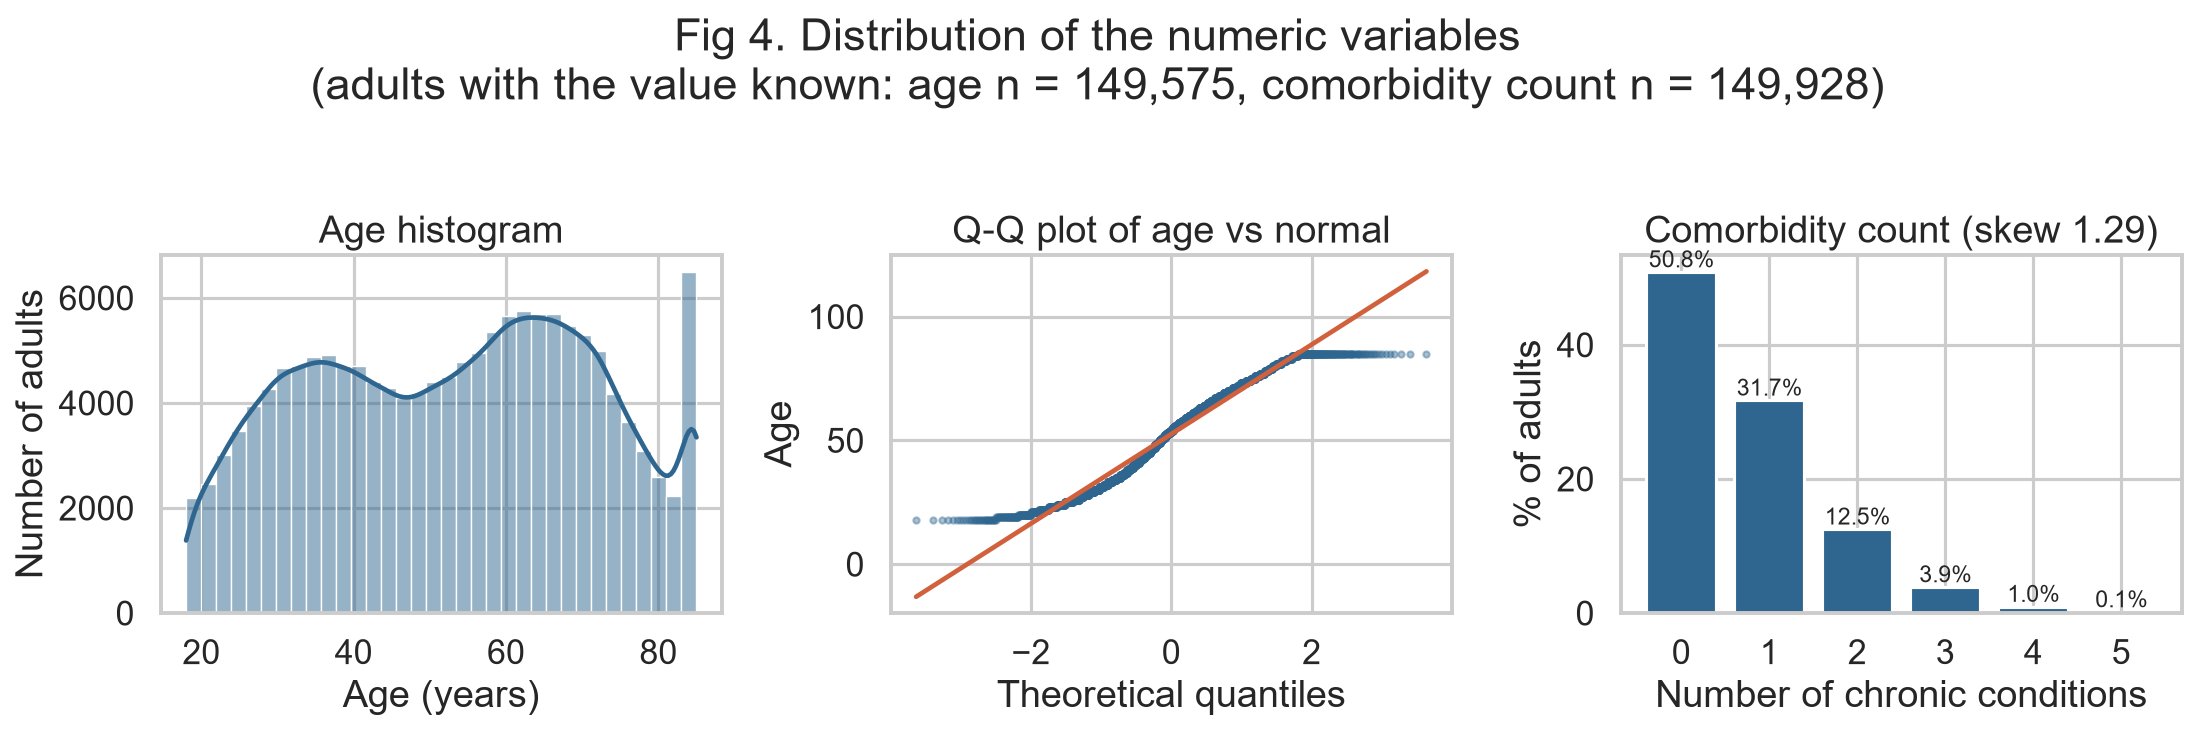
\includegraphics[width=\textwidth]{fig04_numeric_distributions}
\caption{Numeric variables. Left: age histogram (two humps, and a pile-up at 85 = ``85 or older''). Centre: Q-Q plot of age against a normal distribution (the S-shape of a flat distribution). Right: comorbidity count (right-skewed).}\label{fig:numeric}
\end{figure}

\begin{figure}[htbp]
\centering
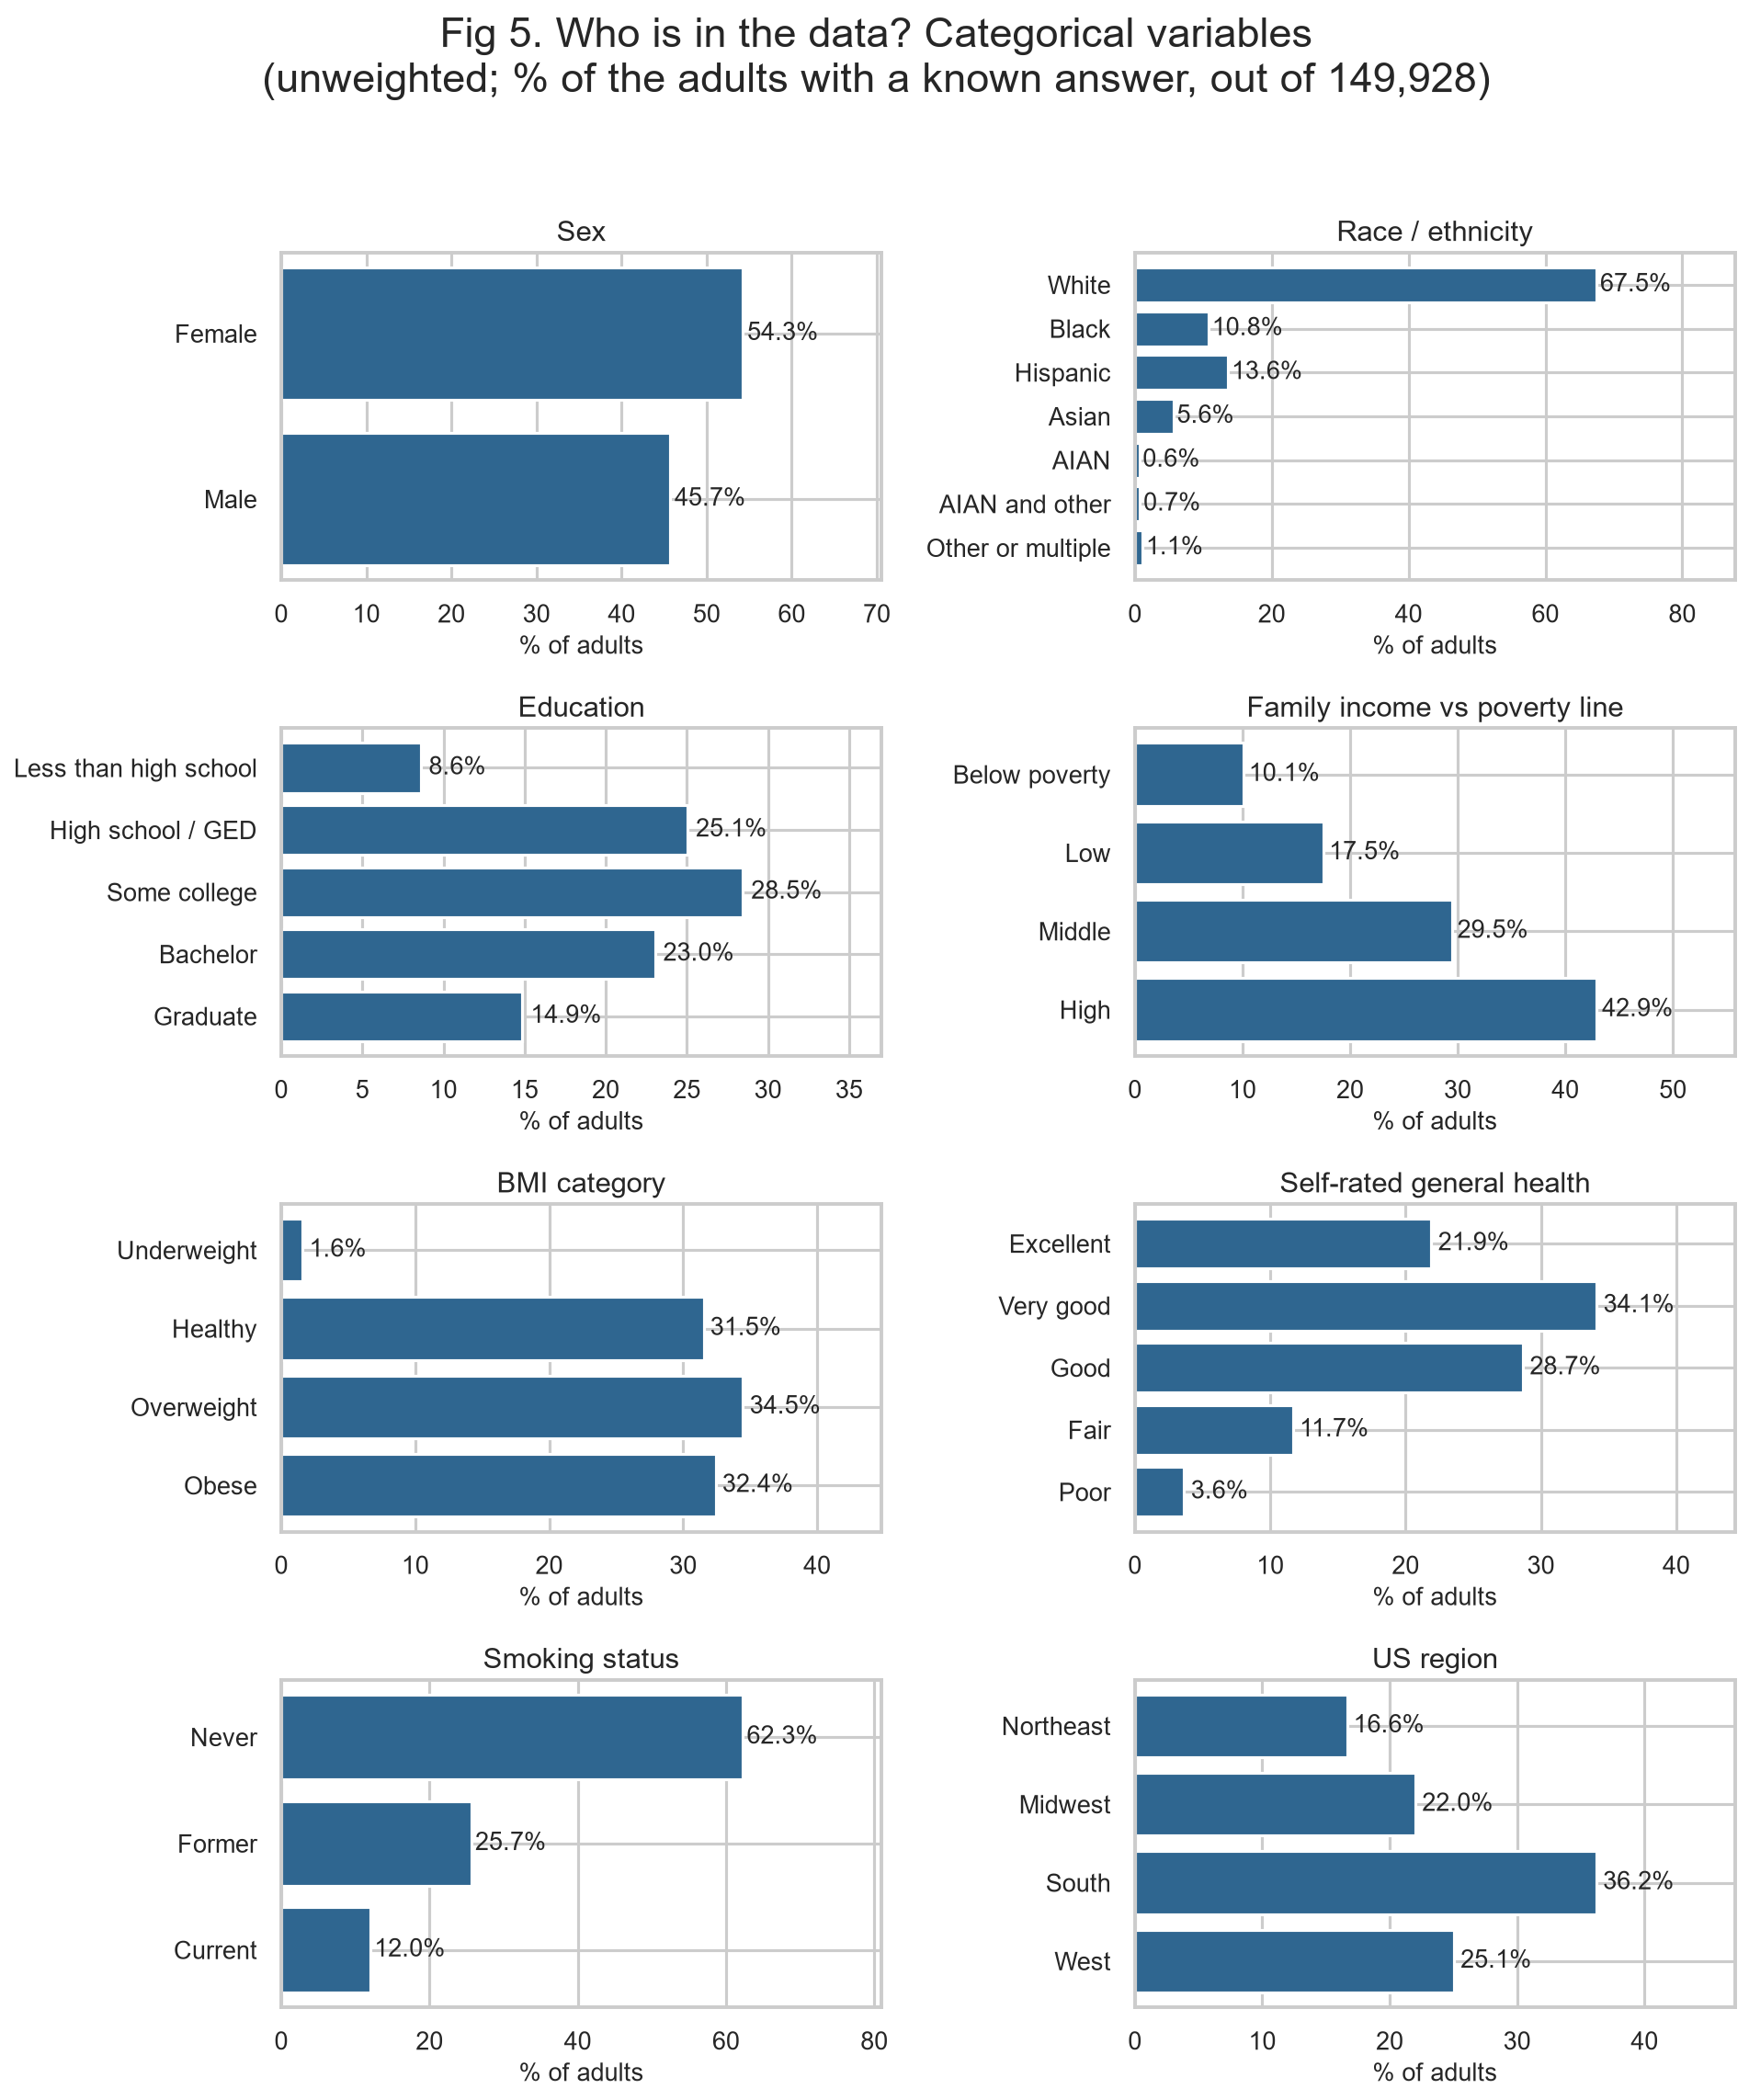
\includegraphics[width=0.85\textwidth]{fig05_categorical_distributions}
\caption{Distribution of the categorical variables (unweighted shares of adults with a known answer). Counts, cases and rates for every category are in Tables~\ref{tab:prof-demo}--\ref{tab:prof-conditions}.}\label{fig:categorical}
\end{figure}

\subsection{RQ1 -- Smoking}\label{sec:rq1}

\begin{table}[htbp]
\centering\small
\caption{Lung-cancer rate by smoking status (absolute risk) and risk ratio against never-smokers (adults with known smoking status).}\label{tab:rate-smoking}
\begin{tabular}{lrrrrr}
\toprule
Smoking status & Adults & Cases & \makecell[b]{Sample\\{}rate} & \makecell[b]{Weighted\\{}(population) rate} & \makecell[b]{Risk ratio\\{}(weighted)} \\
\midrule
Never & 90,937 & 107 & 0.12\% & 0.08\% & 1 (reference) \\
Former & 37,452 & 367 & 0.98\% & 0.81\% & 10.0 \\
Current & 17,586 & 127 & 0.72\% & 0.60\% & 7.4 \\
\bottomrule
\end{tabular}

\end{table}

\begin{itemize}
  \item \textbf{Hypotheses.} H$_0$: smoking status and lung cancer are independent; H$_1$: they are associated.
  \item \textbf{Test and assumption.} Both variables are categorical (a $3 \times 2$ table), so we use Pearson's $\chi^2$ test of independence. Its assumption holds: the smallest expected count is 72.4, far above 5.
  \item \textbf{Result.} $\chi^2(2) = 528.0$, $p = 2.2 \times 10^{-115}$ (Holm $p = 3.1 \times 10^{-114}$), Cram\'er's $V = 0.060$ -- small by Cohen's conventions~\cite{cohen}.
  \item \textbf{Effect size.} Ever-smokers vs never-smokers: odds ratio \orSmokingExact (95\% CI 6.22--9.44). In absolute terms, about 8 in 10,000 never-smokers have a lung-cancer history in the population, against about 81 in 10,000 former and 60 in 10,000 current smokers (Table~\ref{tab:rate-smoking}, Fig.~\ref{fig:smoking}).
  \item \textbf{How we read it.} The tiny $p$-value mostly reflects our sample size, and $V$ looks small because 99.6\% of every group is cancer-free -- $V$ is bounded by the rarity of the outcome. The odds ratio is the meaningful effect size for a rare outcome: ever-smokers have about \orSmoking times the odds of a lung-cancer history.
  \item \textbf{Why former smokers look worse than current ones (0.81\% vs 0.60\%).} At first this looked like a bug, but it is not one. NHIS records smoking now, and many people quit after their diagnosis, which moves them into the ``former'' group (reverse causation). Former smokers are also older (median age 63 vs 52 for current smokers), which is why we look at age next.
\end{itemize}

\begin{figure}[htbp]
\centering
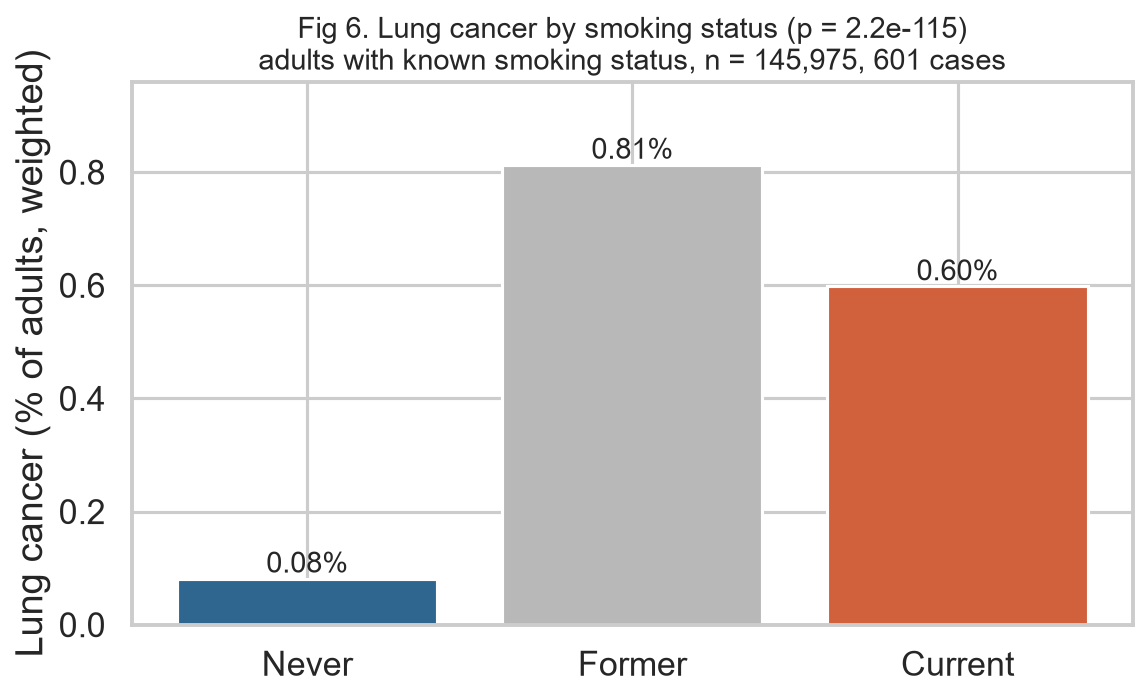
\includegraphics[width=0.6\textwidth]{fig06_smoking_vs_lung_cancer}
\caption{Weighted share of adults with a lung-cancer history, by smoking status (the $p$-value in the title is the raw $\chi^2$ $p$-value).}\label{fig:smoking}
\end{figure}

\subsection{RQ2a -- Age, and how it interacts with smoking}\label{sec:age}

\begin{figure}[htbp]
\centering
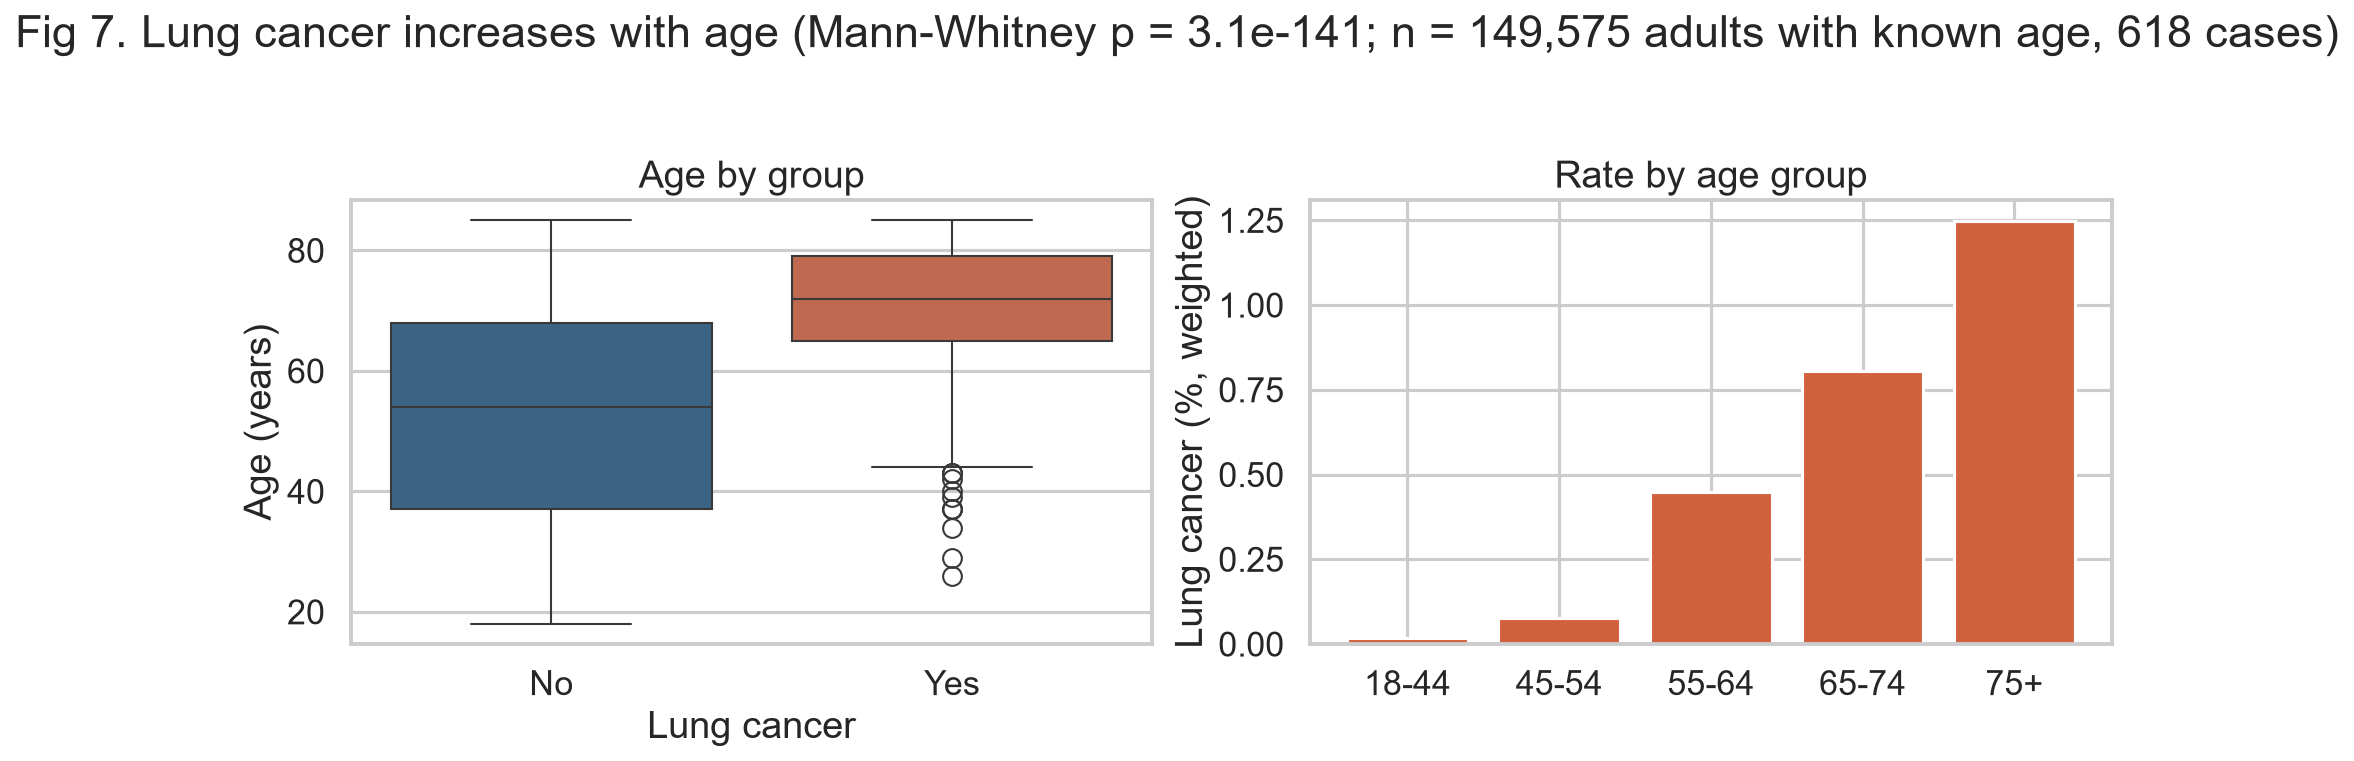
\includegraphics[width=\textwidth]{fig07_age_vs_lung_cancer}
\caption{Left: age distribution with and without lung cancer. Right: weighted lung-cancer rate by age group.}\label{fig:age}
\end{figure}

\begin{itemize}
  \item \textbf{Difference.} The median age is 72 with lung cancer vs 54 without, and the weighted rate rises steadily from the youngest to the oldest age group (Fig.~\ref{fig:age}).
  \item \textbf{Test choice.} H$_0$: both groups have the same age distribution. Age is not normal (\S\ref{sec:univariate}) and the groups are very unequal (618 vs 148,957 adults with a known age), so we use the Mann--Whitney $U$ test rather than a $t$-test.
  \item \textbf{Result.} $U = 73{,}126{,}291$, $p = 3.1 \times 10^{-141}$, rank-biserial $r = 0.59$ -- a large effect. In plain words: if we pick one adult with and one without a lung-cancer history at random, the one with lung cancer is older $(1 + 0.59)/2 \approx 79.5\%$ of the time.
  \item \textbf{Robustness.} With samples this large the $t$-test is also valid (central limit theorem), so we ran Welch's $t$-test as a check: $t = 44.9$, $p = 4.6 \times 10^{-199}$. Both tests agree, so the conclusion does not depend on the choice of test.
\end{itemize}

\begin{figure}[htbp]
\centering
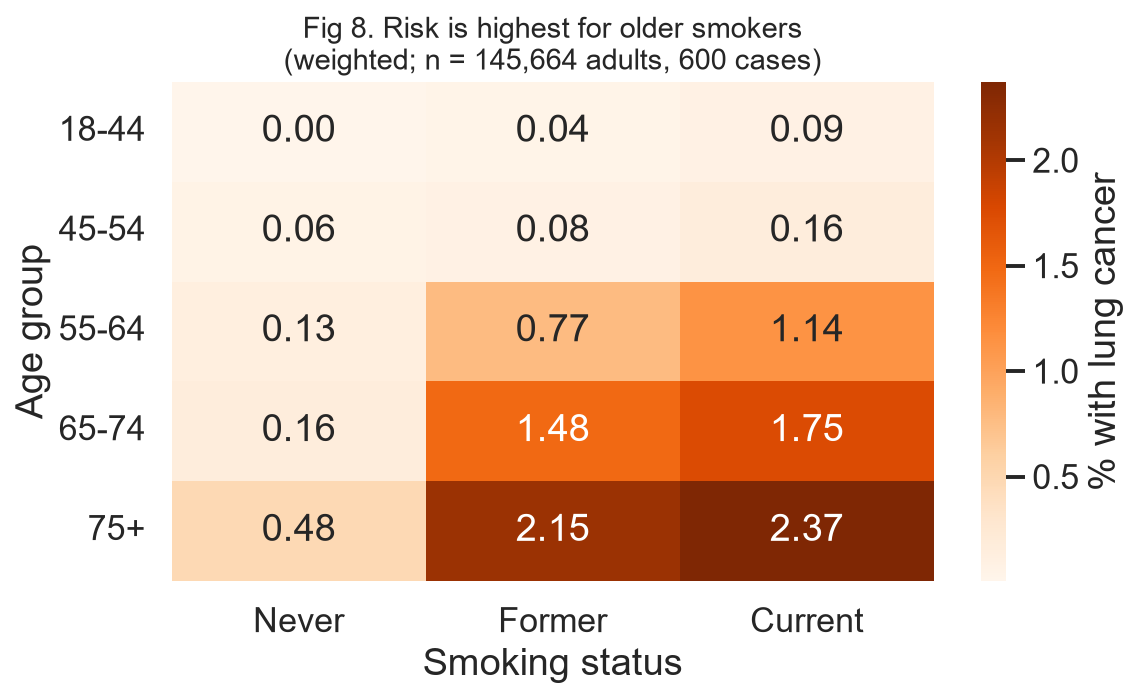
\includegraphics[width=0.6\textwidth]{fig08_age_x_smoking}
\caption{Weighted lung-cancer rate (\%) for each age group and smoking status. Cells for adults under 45 contain very few cases (3 never-smokers and 10 ever-smokers in total), so their rates are imprecise.}\label{fig:agesmoking}
\end{figure}

\begin{itemize}
  \item \textbf{Age and smoking act together.} Never-smokers stay below 0.5\% even at 75+. Ever-smokers go from under 0.1\% before 45 to 2.15\% (former) and 2.37\% (current) at 75+.
  \item \textbf{Smoking is not just age in disguise -- tested.} Because ever-smokers are older, part of the crude odds ratio could be age. We therefore compared ever- with never-smokers inside each age group and pooled the groups with the Cochran--Mantel--Haenszel (CMH) method (Table~\ref{tab:smoking-age}). The odds ratio falls from 7.6 to \orSmokingMH (95\% CI 4.7--7.1) once age group is held fixed, and the CMH test rejects ``no association within age groups'' ($\chi^2 = 340.5$, $p = 5 \times 10^{-76}$). Part of the crude effect was therefore age, but a strong smoking association remains. The Breslow--Day test ($p = 0.005$) shows the size of the effect differs between age groups: it is about 8 from 55 to 74, 4.4 at 75+, and not significant at 45--54 (only 21 cases), so the pooled \orSmokingMH is an average.
  \item This combination of age and smoking is exactly the logic of the USPSTF screening rule, which combines age 50--80 with smoking history -- and the reason we built the \file{screening_age_smoker} feature (\S\ref{sec:created}, Table~\ref{tab:engineered}).
\end{itemize}

\begin{table}[htbp]
\centering\small
\caption{Smoking and lung cancer inside each age group (ever vs never smokers; adults with known smoking status and age). CMH $\chi^2 = 340.5$, $p = 5 \times 10^{-76}$; Breslow--Day $p = 0.005$. Source: \texttt{smoking\_by\_age\_group.csv}.}\label{tab:smoking-age}
\begin{tabular}{lrrrr}
\toprule
Age group & Adults & \makecell[b]{Cases,\\{}ever-smokers} & \makecell[b]{Cases,\\{}never-smokers} & Odds ratio [95\% CI] \\
\midrule
18--44 & 53,022 & 10 & 3 & 7.7 [2.3, 25.9] \\
45--54 & 20,987 & 11 & 10 & 1.9 [0.8, 4.3] \\
55--64 & 26,358 & 96 & 15 & 8.2 [4.8, 14.0] \\
65--74 & 25,842 & 187 & 27 & 7.9 [5.3, 11.7] \\
75+ & 19,455 & 189 & 52 & 4.4 [3.2, 5.9] \\
\midrule
Crude (age ignored) & 145,664 &  &  & 7.6 [6.2, 9.4] \\
Mantel--Haenszel (adjusted for age group) & 145,664 &  &  & 5.8 [4.7, 7.1] \\
\bottomrule
\end{tabular}

\end{table}

\subsection{RQ2b -- Chronic conditions}\label{sec:conditions}

\begin{figure}[htbp]
\centering
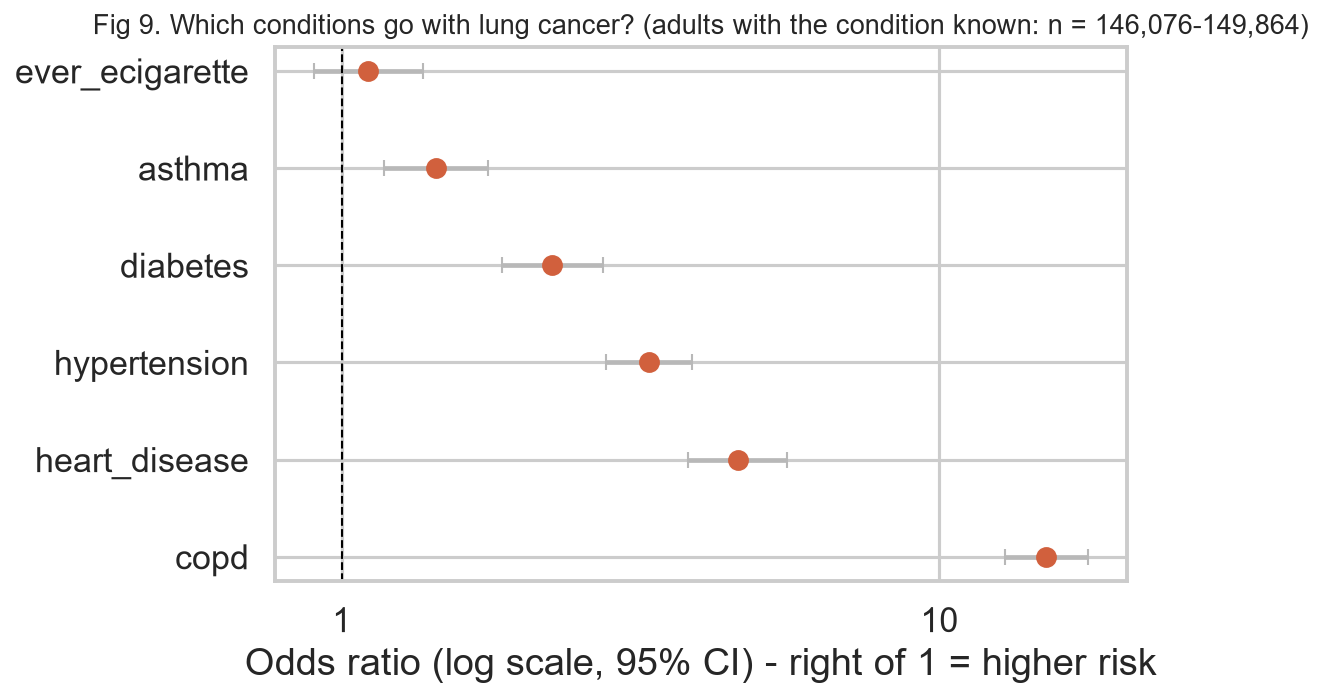
\includegraphics[width=0.65\textwidth]{fig09_odds_ratios_conditions}
\caption{Odds ratio of a lung-cancer history for each condition, with 95\% confidence intervals (log scale). Right of 1 means higher odds.}\label{fig:conditions}
\end{figure}

\begin{table}[htbp]
\centering\small
\caption{Chronic conditions and e-cigarette use vs lung cancer ($\chi^2$ tests; all expected counts $\geq 5$).}\label{tab:conditions}
\begin{tabular}{lrrrrr}
\toprule
Condition & \makecell[b]{Rate\\{}if yes} & \makecell[b]{Rate\\{}if no} & \makecell[b]{Odds ratio\\{}[95\% CI]} & Cram\'er's $V$ & Holm $p$ \\
\midrule
COPD & 3.41\% & 0.23\% & 15.1 [12.9, 17.7] & 0.114 & $<10^{-300}$ \\
Heart disease & 1.53\% & 0.34\% & 4.6 [3.8, 5.6] & 0.045 & $7.3\times10^{-65}$ \\
Hypertension & 0.74\% & 0.23\% & 3.3 [2.8, 3.9] & 0.038 & $1.5\times10^{-48}$ \\
Diabetes & 0.82\% & 0.36\% & 2.3 [1.9, 2.7] & 0.022 & $6.7\times10^{-16}$ \\
Asthma & 0.56\% & 0.39\% & 1.4 [1.2, 1.8] & 0.009 & $2.9\times10^{-3}$ \\
E-cigarette (ever) & 0.45\% & 0.41\% & 1.1 [0.9, 1.4] & 0.002 & 1.00 \\
\bottomrule
\end{tabular}

\end{table}

\begin{itemize}
  \item \textbf{COPD is the strongest signal in the whole project.} It shares smoking as a cause and is also a known risk factor on its own -- which is why we test it against smoking (and age) in \S\ref{sec:copd}.
  \item \textbf{Heart disease, hypertension and diabetes} are partly proxies for age; these odds ratios (Fig.~\ref{fig:conditions}) are not age-adjusted, so we do not over-read them.
  \item \textbf{Asthma} survives correction, but its effect is negligible ($V = 0.009$): a clear example of significant without being important.
  \item \textbf{E-cigarette use shows nothing} (raw $p = 0.39$, Holm $p = 1.00$). That makes sense: e-cigarettes are recent, users are mostly young (mean age 41 vs 55 for non-users, Table~\ref{tab:prof-smoking}), and lung cancer takes decades to develop. Section~\ref{sec:notshow} reports what this null result can and cannot rule out.
\end{itemize}

\subsection{RQ2b -- Is the COPD link only due to smoking?}\label{sec:copd}

Smokers develop COPD more often and lung cancer more often, so smoking alone could create a COPD--lung-cancer association -- a classic confounder. To separate the two, we compared adults with and without COPD within each smoking group (Fig.~\ref{fig:copd}, Table~\ref{tab:copd-smoking}), then pooled the three groups with the Cochran--Mantel--Haenszel (CMH) test~\cite{mantel}, which tests H$_0$: ``no COPD--lung-cancer association once smoking status is held fixed''.

\begin{figure}[htbp]
\centering
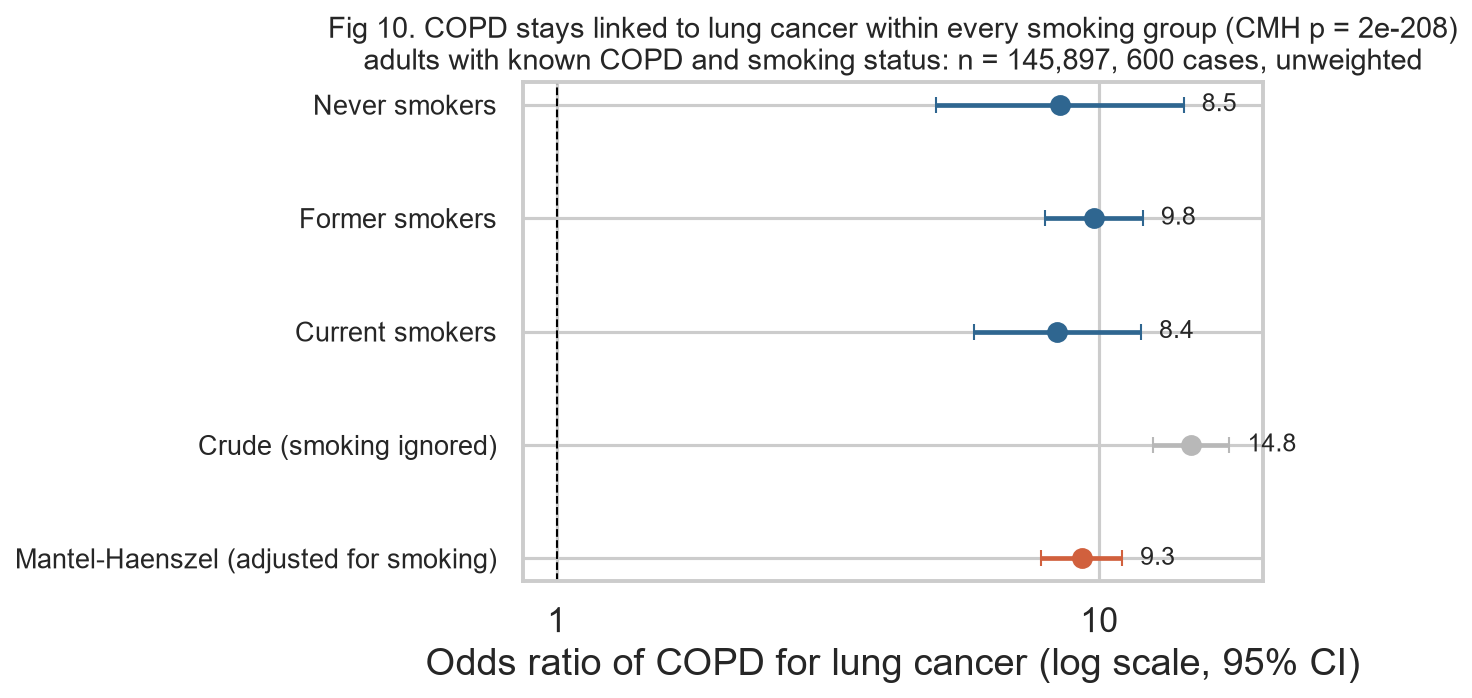
\includegraphics[width=0.75\textwidth]{fig10_copd_stratified_by_smoking}
\caption{Odds ratio of COPD for lung cancer within each smoking group, ignoring smoking (crude) and adjusted for smoking (Mantel--Haenszel), with 95\% confidence intervals (log scale).}\label{fig:copd}
\end{figure}

\begin{table}[htbp]
\centering\small
\caption{COPD and lung cancer, stratified by smoking status (adults with known COPD and smoking status).}\label{tab:copd-smoking}
\begin{tabular}{lrrr}
\toprule
Group & Adults & Cases & Odds ratio [95\% CI] \\
\midrule
Never smokers & 90,901 & 107 & 8.5 [5.0, 14.3] \\
Former smokers & 37,424 & 366 & 9.8 [7.9, 12.0] \\
Current smokers & 17,572 & 127 & 8.4 [5.9, 11.9] \\
\midrule
Crude (smoking ignored) & 145,897 & 600 & 14.8 [12.6, 17.4] \\
Mantel--Haenszel (adjusted for smoking) & 145,897 & 600 & 9.3 [7.8, 11.0] \\
\bottomrule
\end{tabular}

\end{table}

\begin{itemize}
  \item \textbf{CMH test:} $\chi^2 = 949.7$, $p = 1.5 \times 10^{-208}$ (Holm $p = 2.4 \times 10^{-207}$) -- the association survives adjustment for smoking.
  \item \textbf{Breslow--Day test} of equal odds ratios across the three groups: $p = 0.69$, so the effect is consistent across groups and pooling them is justified.
  \item \textbf{How we read it.} The crude odds ratio of these 145,897 adults is \orCOPDcrude (slightly below the \orCOPD of Table~\ref{tab:conditions}, which uses everyone with a known COPD answer); it falls to \orCOPDsmoking once smoking is held fixed, so part of the crude association was due to smoking. But COPD remains strongly associated with lung cancer in never, former and current smokers alike -- even never-smokers with COPD have 8.5 times the odds.
  \item \textbf{Age as a second confounder.} Adults with COPD are much older (mean age 65.4 vs 52.0). On the 145,587 adults whose age is also known (599 cases), the crude odds ratio is 14.7 and the smoking-adjusted one 9.2 -- the same picture as above -- and stratifying by smoking status and age group together (15 strata; Table~\ref{tab:copd-adjusted}) lowers it further, to \orCOPDsmokingAge (95\% CI 4.8--6.8), still highly significant ($\chi^2 = 501.9$, $p = 3.7 \times 10^{-111}$). COPD is therefore strongly associated with lung cancer beyond what smoking and age explain -- still an association, not a cause.
\end{itemize}

\begin{table}[htbp]
\centering\small
\caption{COPD odds ratio under increasing adjustment (the 145,587 adults with known COPD, smoking status and age; 599 cases). Source: \texttt{copd\_adjusted.csv}.}\label{tab:copd-adjusted}
\begin{tabular}{lr}
\toprule
Adjusted for & Odds ratio [95\% CI] \\
\midrule
None (crude) & 14.7 [12.5, 17.3] \\
Smoking status (3 strata) & 9.2 [7.8, 11.0] \\
Smoking status $\times$ age group (15 strata) & 5.7 [4.8, 6.8] \\
\bottomrule
\end{tabular}

\end{table}

\subsection{RQ2c -- Socio-demographic and health factors}\label{sec:sociodemo}

\begin{figure}[htbp]
\centering
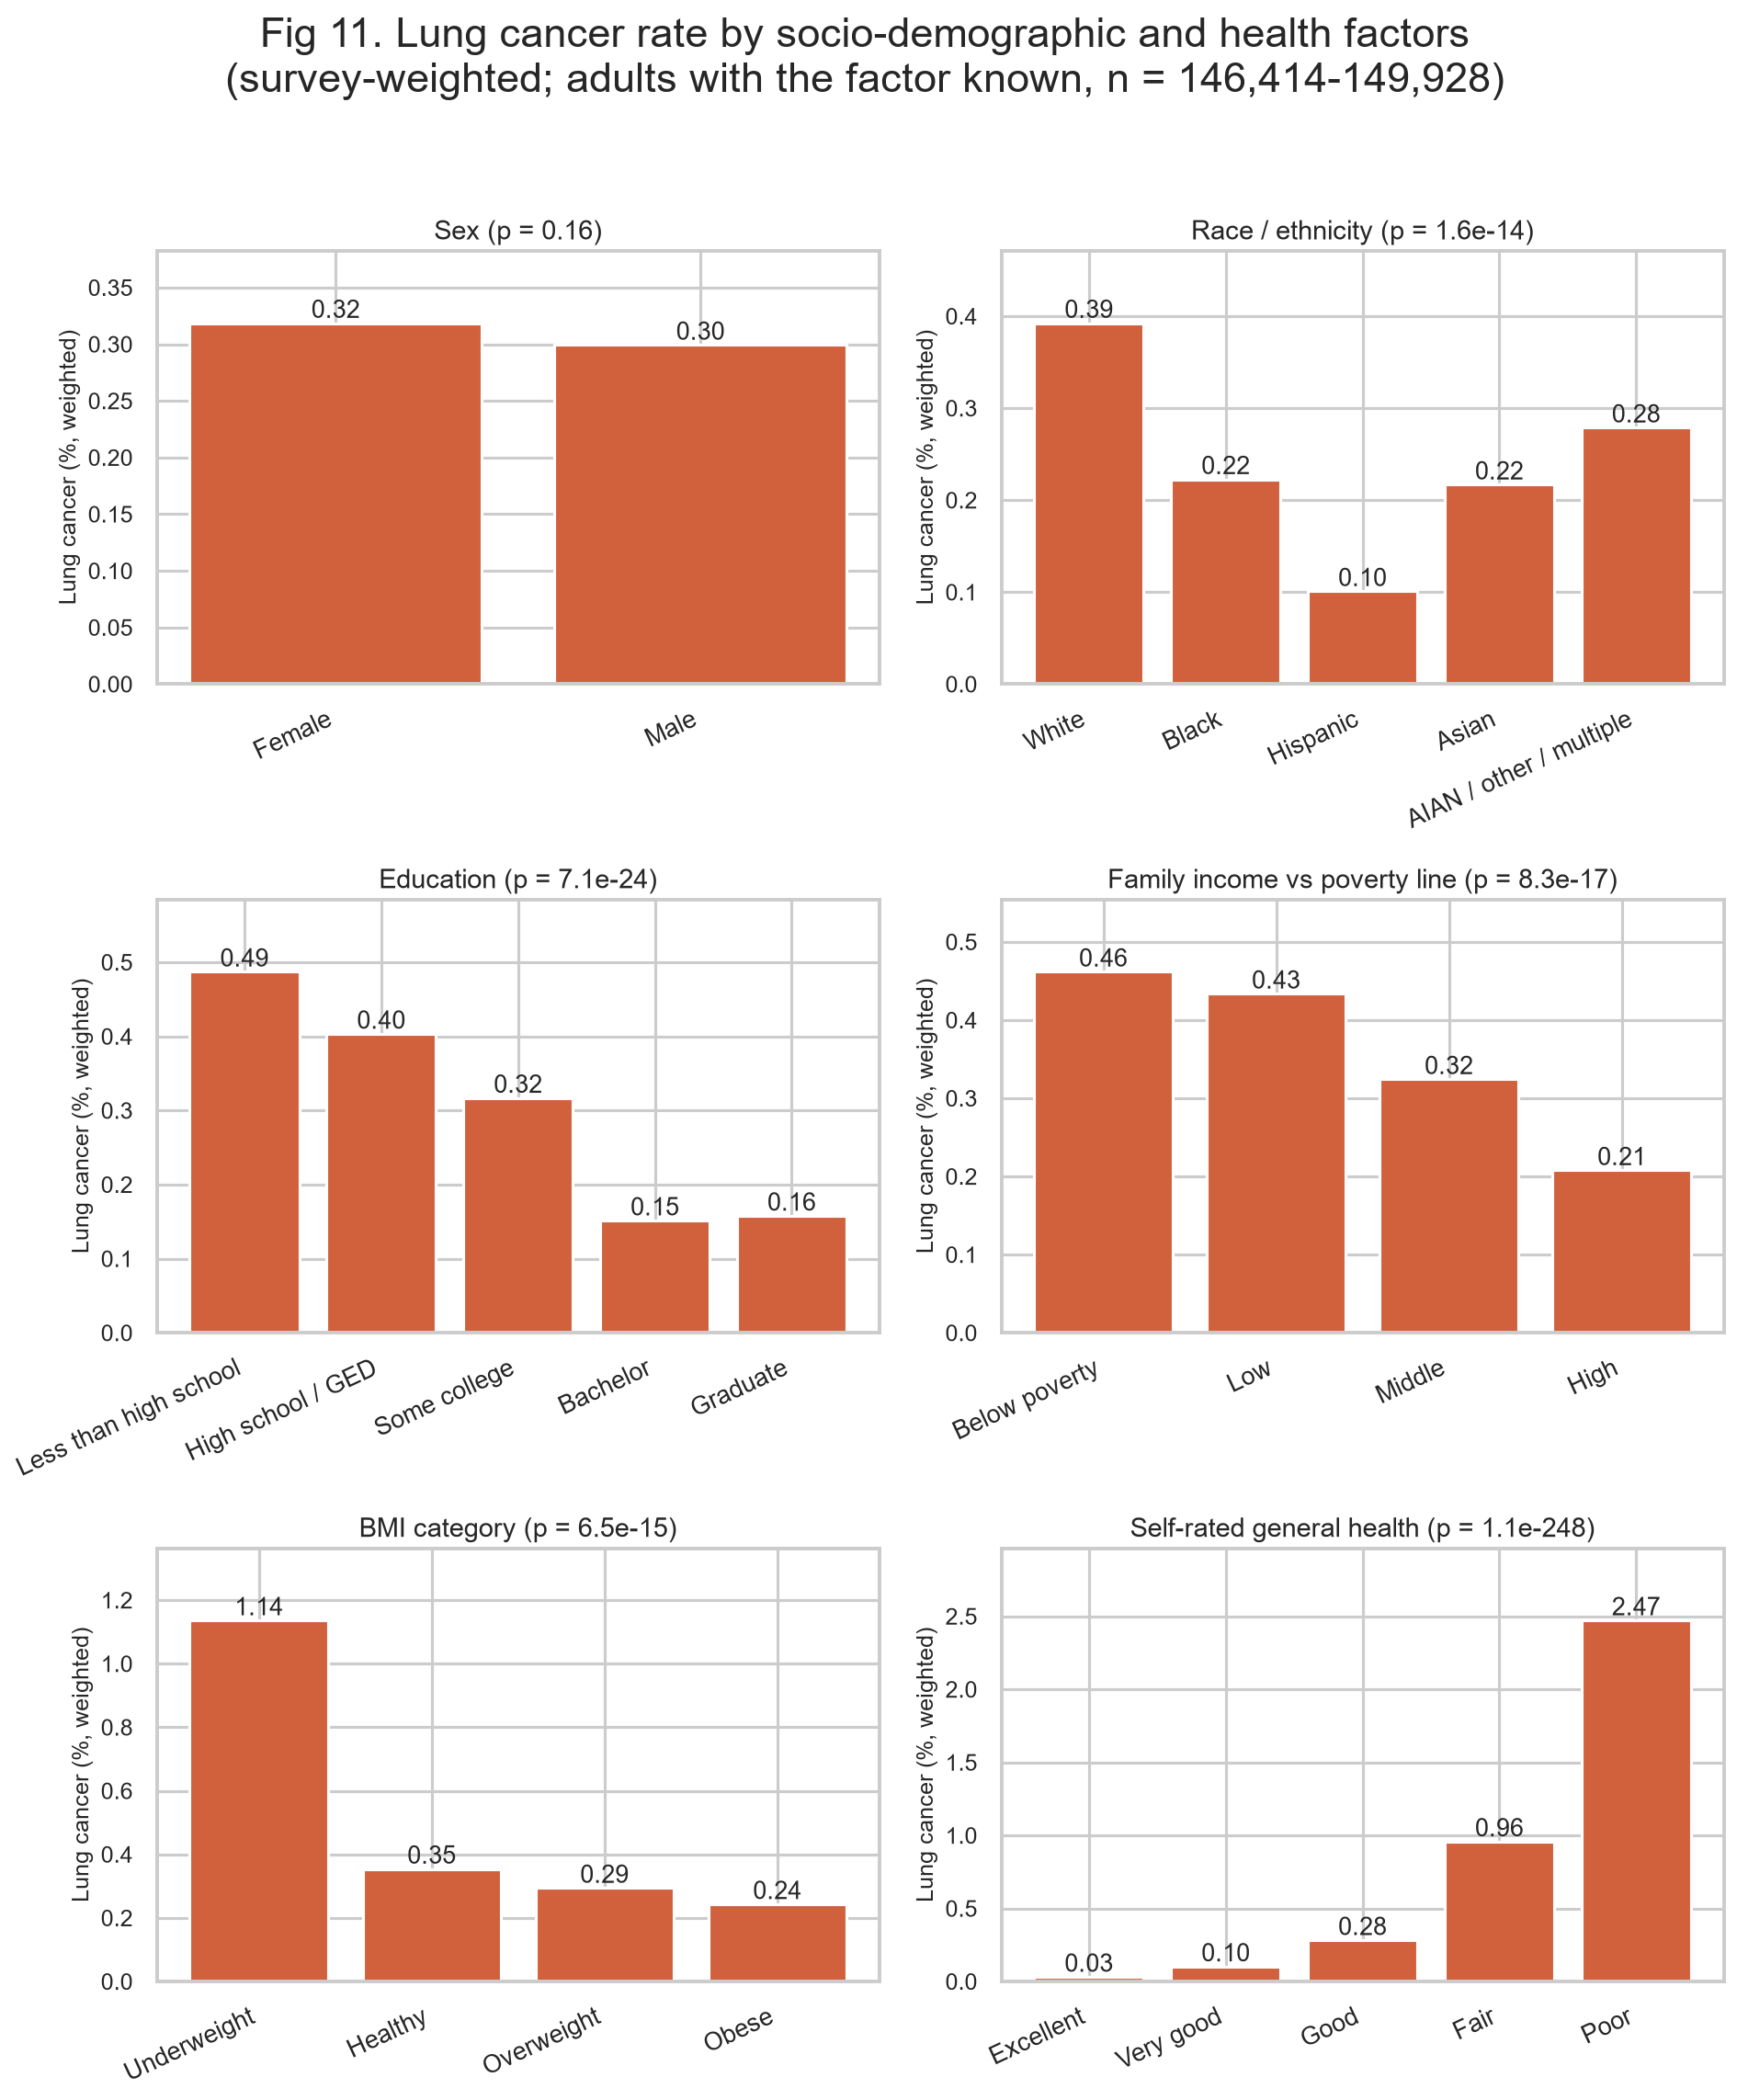
\includegraphics[width=0.85\textwidth]{fig11_demographics_vs_lung_cancer}
\caption{Weighted lung-cancer rate (\%) by sex, race/ethnicity, education, income, BMI category and self-rated general health, with the raw $\chi^2$ $p$-value of each test in the panel titles (Holm-adjusted values in Table~\ref{tab:demographics}).}\label{fig:demographics}
\end{figure}

\begin{table}[htbp]
\centering\small
\caption{Socio-demographic and health factors vs lung cancer ($\chi^2$ tests of independence). The three smallest race groups (AIAN, AIAN and other, Other or multiple; 2.5\% of adults) were merged for the test, because their expected case counts fell below 5 (smallest 4.0), which makes the $\chi^2$ approximation unreliable. After merging, the smallest expected count is 15.5. The model-ready file keeps all seven groups as categories (White is the reference category).}\label{tab:demographics}
\begin{tabularx}{\textwidth}{l >{\raggedright\arraybackslash}X r r r}
\toprule
Factor & Weighted rate: highest $\rightarrow$ lowest group & $\chi^2$ (df) & Holm $p$ & Cram\'er's $V$ \\
\midrule
Sex & Female 0.32\% $\rightarrow$ Male 0.30\% & 2.0 (1) & 0.62 & 0.004 \\
Race / ethnicity & White 0.39\% $\rightarrow$ Hispanic 0.10\% & 70.7 (4) & $1.1\times10^{-13}$ & 0.022 \\
Education & Less than high school 0.49\% $\rightarrow$ Bachelor 0.15\% & 114.7 (4) & $7.8\times10^{-23}$ & 0.028 \\
Income vs poverty line & Below poverty 0.46\% $\rightarrow$ High 0.21\% & 78.0 (3) & $7.5\times10^{-16}$ & 0.023 \\
BMI category & Underweight 1.14\% $\rightarrow$ Obese 0.24\% & 69.2 (3) & $5.2\times10^{-14}$ & 0.022 \\
Self-rated health & Poor 2.47\% $\rightarrow$ Excellent 0.03\% & 1,154.7 (4) & $1.8\times10^{-247}$ & 0.088 \\
\bottomrule
\end{tabularx}

\end{table}

\begin{itemize}
  \item \textbf{Sex} is not associated with lung cancer here (raw $p = 0.16$, Holm $p = 0.62$; Table~\ref{tab:demographics}).
  \item \textbf{A social gradient.} Less education and lower income go with higher rates (Fig.~\ref{fig:demographics}). Smoking follows the same gradient -- 46\% of adults without a high-school diploma have ever smoked, against 28\% of bachelor's graduates, and 44\% below the poverty line against 33\% in the high-income group -- so part of this gradient is the smoking effect again.
  \item \textbf{Underweight and poor self-rated health have the highest rates.} This is most likely reverse causation: cancer and its treatment cause weight loss and poor health, not the other way round. These features describe people who are already sick, which matters for the modelling phase (\S\ref{sec:final}).
  \item \textbf{Race differences} may partly reflect differences in age and smoking between groups (Table~\ref{tab:group-profile}); they are not adjusted here. All Cram\'er's $V$ values are small, again because the outcome is rare. These tests treat education, income, BMI and health as nominal; a trend test that uses their order would be more powerful, which can only strengthen these already significant results.
\end{itemize}

\subsection{Correlations between variables}\label{sec:correlations}

\begin{figure}[htbp]
\centering
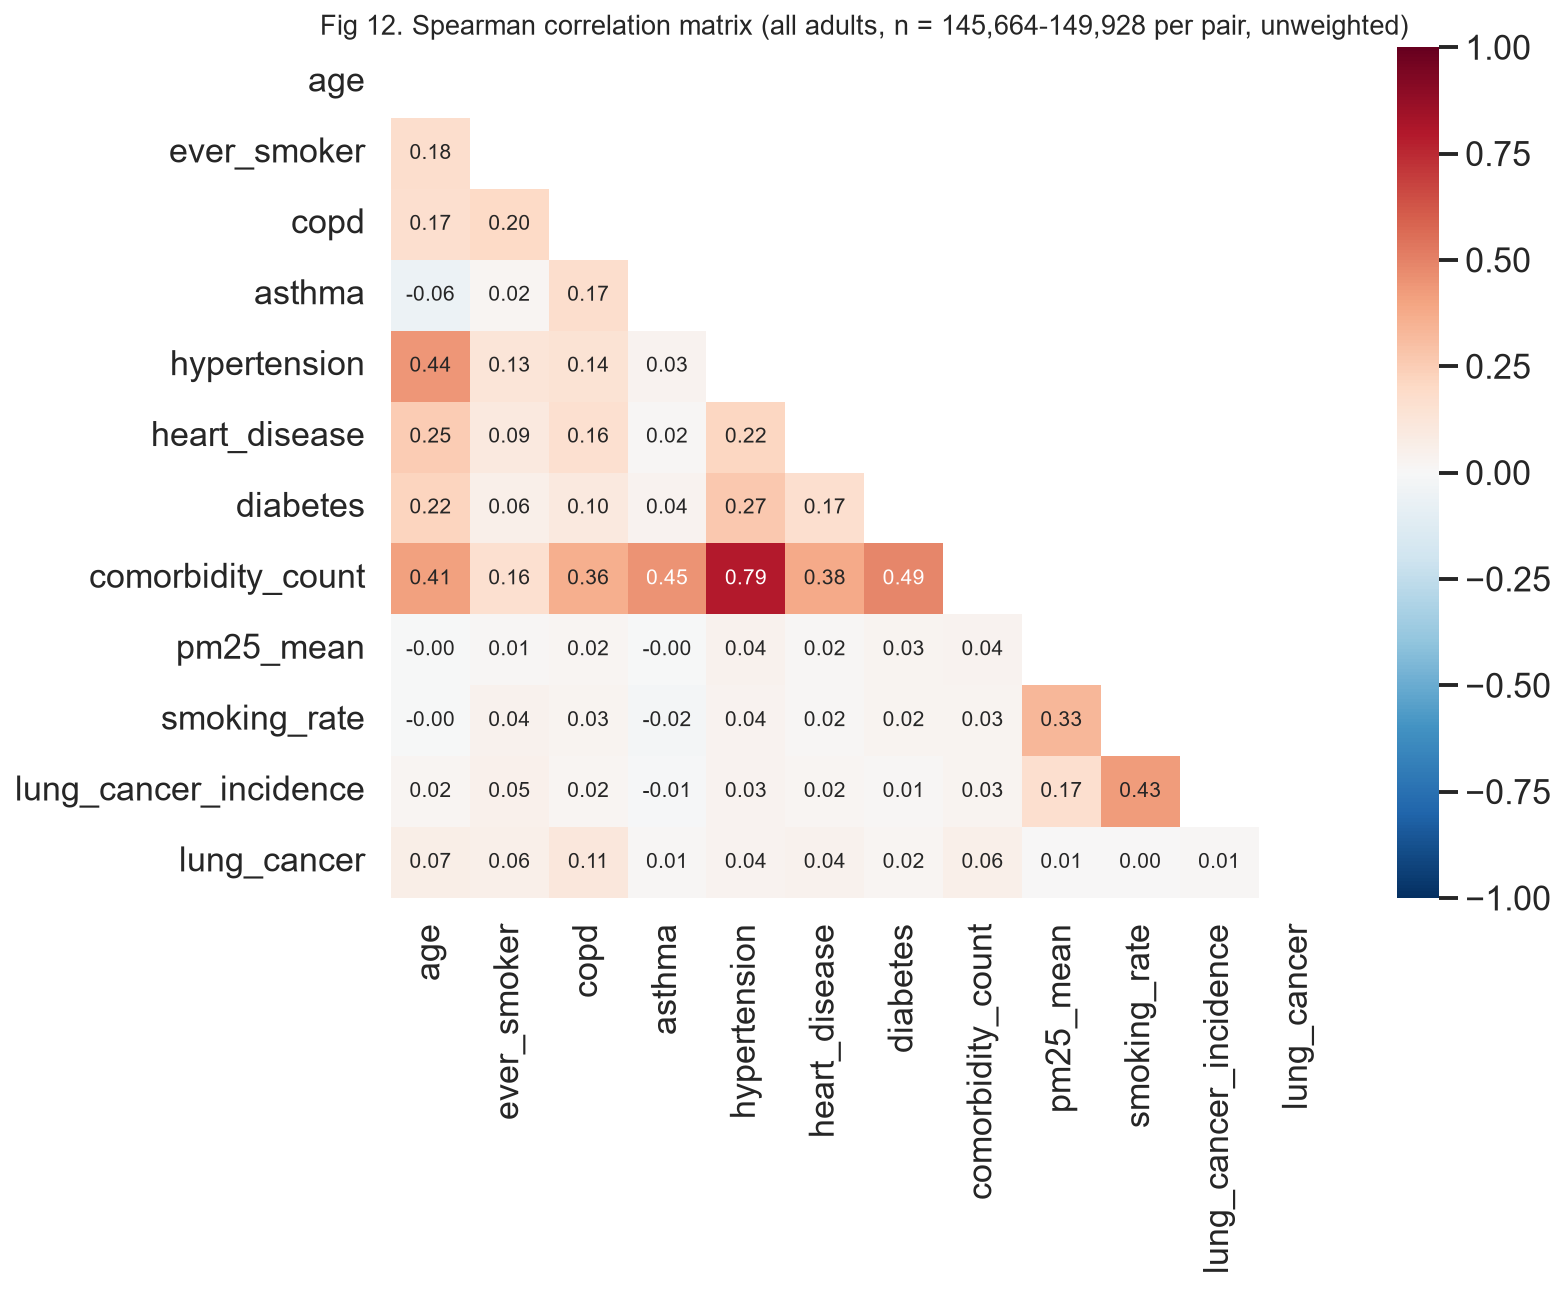
\includegraphics[width=0.7\textwidth]{fig12_correlation_heatmap}
\caption{Spearman correlation matrix of the numeric and binary variables (lower triangle; all adults, unweighted; each pair uses the adults with both values known, $n$ = 145,664--149,928).}\label{fig:corr}
\end{figure}

\begin{itemize}
  \item \textbf{Why Spearman.} Most columns are 0/1 or ordinal, and age is not normal; Spearman uses ranks and only assumes a monotonic relationship, whereas Pearson assumes linearity (Chapter~4).
  \item \textbf{The strongest pairs are expected.} Hypertension--comorbidity count (0.79), diabetes--comorbidity count (0.49) and asthma--comorbidity count (0.45) are high because the count is built from those columns. Age also goes with hypertension (0.44) and the comorbidity count (0.41), and the regional smoking rate with registry incidence (0.43).
\end{itemize}

\begin{figure}[p]
\centering
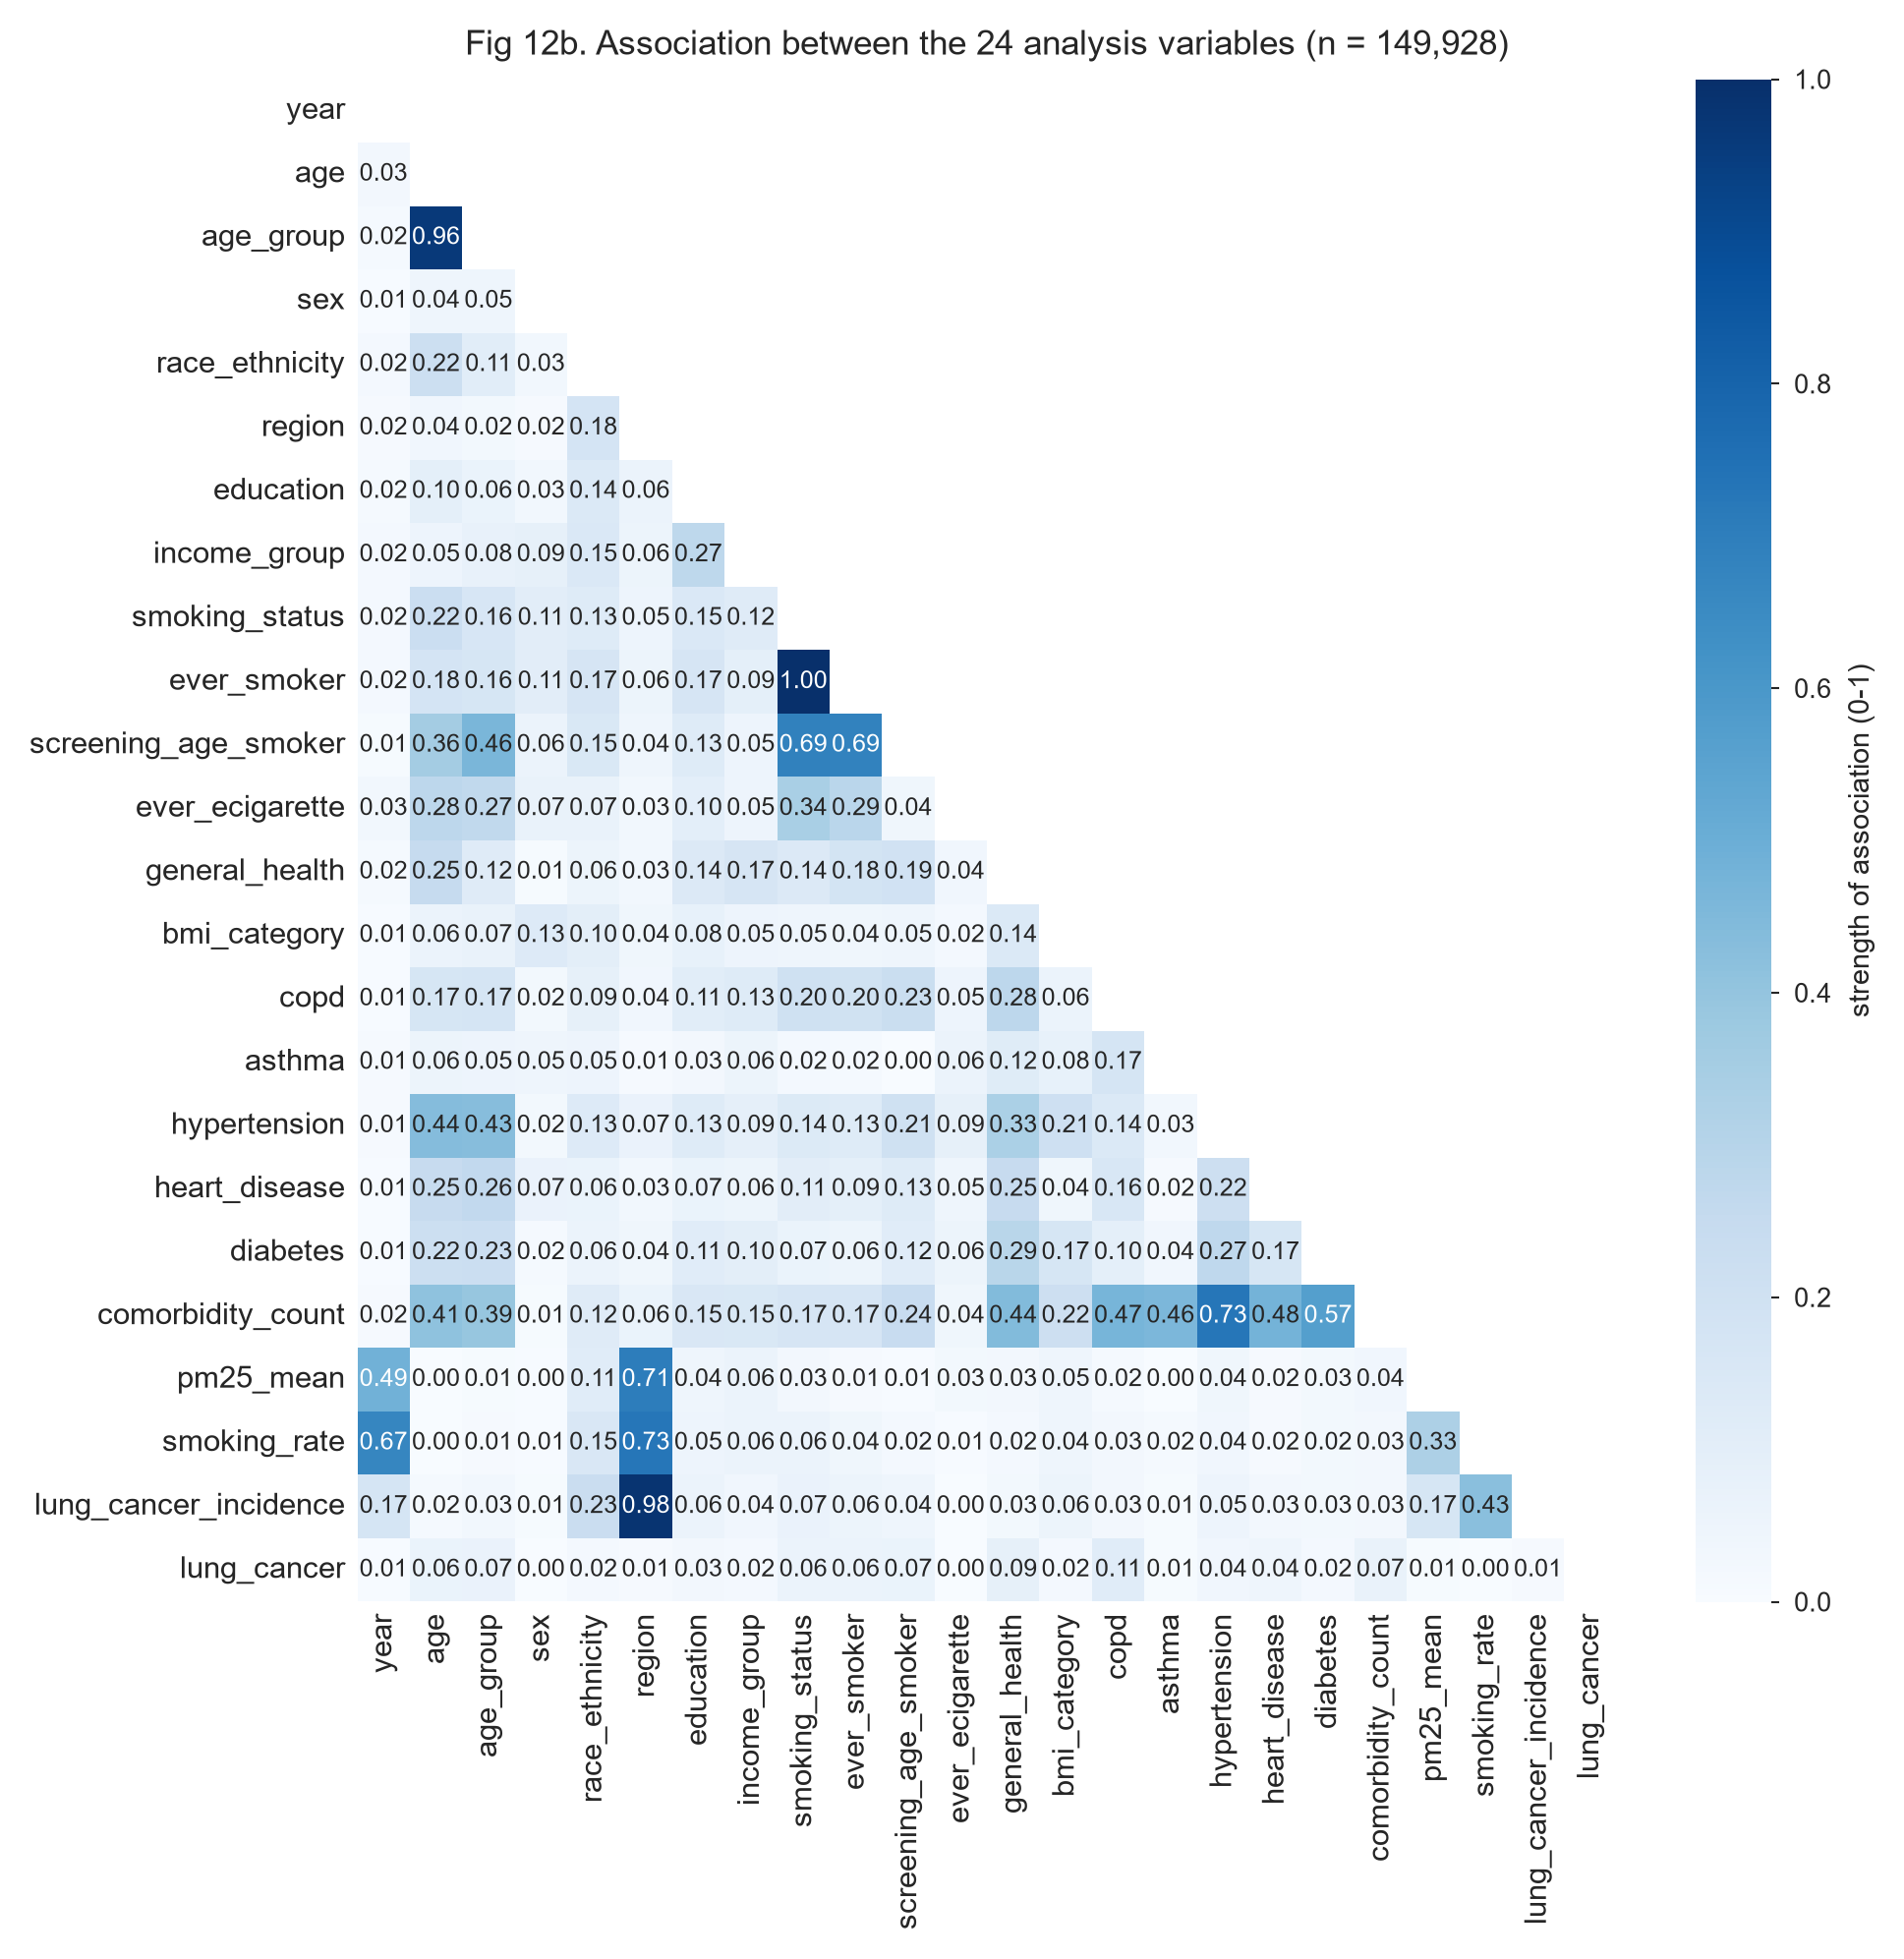
\includegraphics[width=\textwidth]{fig12b_association_matrix}
\figsuffix{b}
\caption{Association between all 24 analysis variables of the clean dataset and the target (all \nAdults adults, \nCases cases; each pair uses the adults with both values known, $n$ = 142,511--149,928; unweighted). Cram\'er's $V$ for two categorical variables, the correlation ratio $\eta$ for a categorical and a numeric variable, $|\text{Spearman}|$ for two numeric variables; all three run from 0 to 1. \texttt{person\_id} and \texttt{survey\_weight} are excluded, and \texttt{CANEV\_A} is not in the clean dataset.}\label{fig:assoc}
\end{figure}

\begin{figure}[p]
\centering
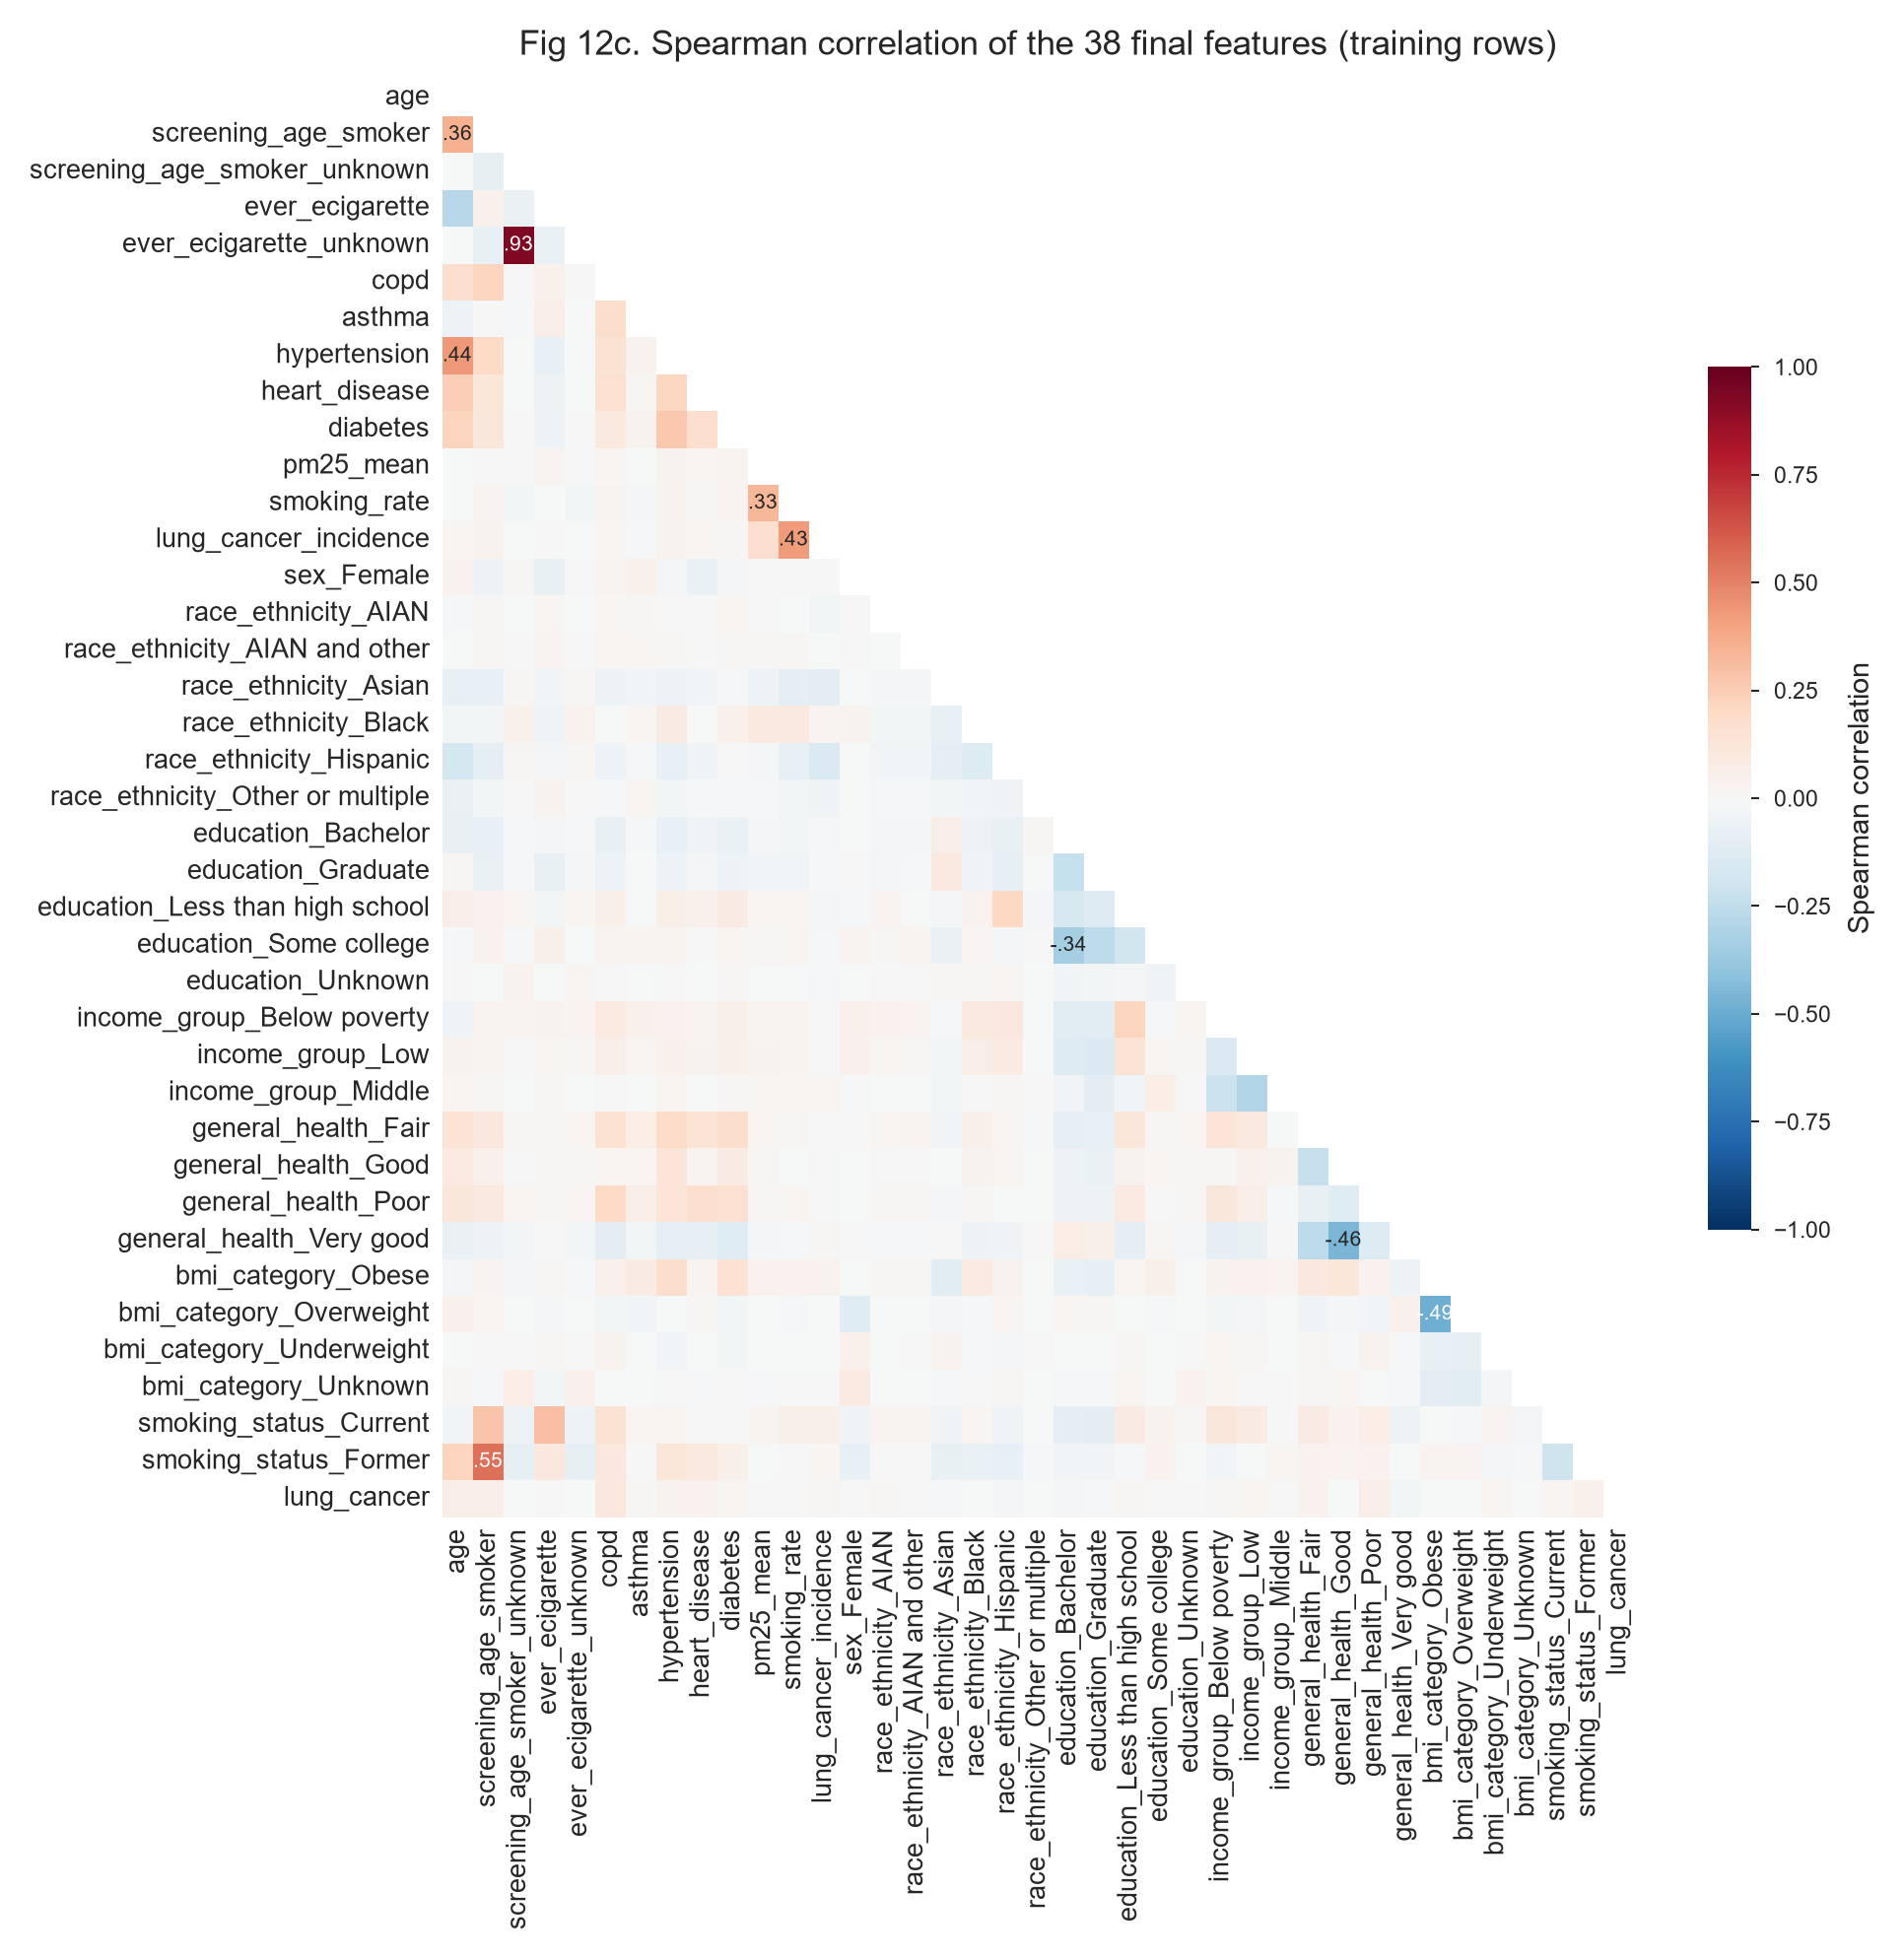
\includegraphics[width=\textwidth]{fig12c_feature_correlation}
\figsuffix{c}
\caption{Spearman correlation of the \nFeatures final model features and the target, on the training rows only ($n$ = \nTrain adults, \nTrainCases cases; unweighted; lower triangle; values printed where $|r| \geq 0.3$).}\label{fig:featcorr}
\end{figure}

Fig.~\ref{fig:corr} only holds the numeric and 0/1 columns, so it cannot show how the categorical variables relate to each other or to the target. Fig.~\ref{fig:assoc} therefore covers \emph{all} 24 analysis variables, with the measure that suits each pair of types, and Fig.~\ref{fig:featcorr} covers \emph{all} \nFeatures features handed to the modelling phase. Every pair above 0.5 in either matrix is listed in Table~\ref{tab:high-pairs} with the reason it is high (\file{results/tables/high_correlation_pairs.csv}).

\begin{table}[htbp]
\centering\footnotesize
\caption{Every pair of variables (Fig.~\ref{fig:assoc}) or features (Fig.~\ref{fig:featcorr}) with an association above 0.5.}\label{tab:high-pairs}
\begin{tabularx}{\textwidth}{l >{\raggedright\arraybackslash}p{4.2cm} l r l >{\raggedright\arraybackslash}X}
\toprule
Matrix & Pair & Measure & Value & Type & Why it is high \\
\midrule
Fig.~12b & year -- smoking\_\allowbreak{}rate & $\eta$ & 0.67 & built-from & smoking\_rate is joined on region + year, and BRFSS smoking fell every year 2019--2023 \\
Fig.~12b & age -- age\_\allowbreak{}group & $\eta$ & 0.96 & built-from & age\_group is age cut into bands \\
Fig.~12b & region -- pm25\_\allowbreak{}mean & $\eta$ & 0.71 & built-from & pm25\_mean is joined on region + year (20 values) \\
Fig.~12b & region -- smoking\_\allowbreak{}rate & $\eta$ & 0.73 & built-from & smoking\_rate is joined on region + year (20 values) \\
Fig.~12b & region -- lung\_\allowbreak{}cancer\_\allowbreak{}incidence & $\eta$ & 0.98 & built-from & lung\_cancer\_incidence is joined on region + year; the West is far lower than the other regions \\
Fig.~12b & smoking\_\allowbreak{}status -- ever\_\allowbreak{}smoker & Cram\'er's $V$ & 1.00 & built-from & ever\_smoker = Current or Former smoking\_status \\
Fig.~12b & smoking\_\allowbreak{}status -- screening\_\allowbreak{}age\_\allowbreak{}smoker & Cram\'er's $V$ & 0.69 & built-from & screening\_age\_smoker = aged 50--80 AND ever smoked \\
Fig.~12b & ever\_\allowbreak{}smoker -- screening\_\allowbreak{}age\_\allowbreak{}smoker & Cram\'er's $V$ & 0.69 & built-from & screening\_age\_smoker = aged 50--80 AND ever smoked \\
Fig.~12b & hypertension -- comorbidity\_\allowbreak{}count & $\eta$ & 0.73 & built-from & comorbidity\_count is the sum of the 5 condition flags, hypertension the most common (36.5\%) \\
Fig.~12b & diabetes -- comorbidity\_\allowbreak{}count & $\eta$ & 0.57 & built-from & comorbidity\_count is the sum of the 5 condition flags \\
Fig.~12c & screening\_\allowbreak{}age\_\allowbreak{}smoker\_\allowbreak{}unknown -- ever\_\allowbreak{}ecigarette\_\allowbreak{}unknown & Spearman & 0.93 & same-concept & both flag the same $\sim$2.8\% of adults who skipped the smoking / tobacco questions \\
Fig.~12c & screening\_\allowbreak{}age\_\allowbreak{}smoker -- smoking\_\allowbreak{}status\_\allowbreak{}Former & Spearman & 0.55 & built-from & screening\_age\_smoker is built from smoking status, and most former smokers are aged 50--80 \\
\bottomrule
\end{tabularx}

\end{table}

\begin{itemize}
  \item \textbf{Redundancy -- what is high, and what we did about it.} All twelve pairs above 0.5 are either \emph{built-from} (one column is computed from the other, or both are joined on region + year; 11 pairs) or \emph{same-concept} (two flags for the same missing block; 1 pair). \textbf{No two separately measured personal variables are associated above 0.5.} The built-from overlaps are handled in feature selection: \file{ever_smoker} and the age bands are dropped by rule 1, and \file{comorbidity_count} and the region dummies by the new rule 4 (\S\ref{sec:selection}). The two high pairs left among the final features are kept on purpose: the two ``unknown'' flags, which together identify adults with an unknown smoking status (\S\ref{sec:final}), and \file{screening_age_smoker} with former smoking, because the screening rule needs smoking status and age together. Both have a variance inflation factor below 10 (Table~\ref{tab:vif}). Pairwise matrices also have a blind spot: a column can be an exact combination of \emph{several} others (the comorbidity count is the sum of five flags; every complete one-hot group sums to 1) without any single pair exceeding 0.5. Hypertension--comorbidity count was the only visible trace of such a dependency in Fig.~\ref{fig:corr} (Spearman 0.79). This is why feature selection now also checks the VIF (\S\ref{sec:selection}).
  \item \textbf{Why every correlation with the target is small.} Nothing correlates strongly with the target (Fig.~\ref{fig:corr}: highest COPD 0.11, age 0.07; Fig.~\ref{fig:assoc}: COPD 0.11, general health 0.09). This is a property of a rare outcome, not a sign that the factors are weak. For two 0/1 variables, Spearman, Pearson and $\varphi$ coincide, and $\varphi$ can only reach 1 when both have the same prevalence. A feature with prevalence $q$ can reach at most $\varphi_{\max} = \sqrt{p(1-q) / \bigl(q(1-p)\bigr)}$ with a target of prevalence $p = \sampleRate\%$. COPD (5.6\% of adults) can therefore reach at most 0.26, and its observed 0.11 is 43\% of that maximum, with an odds ratio of \orCOPD (Table~\ref{tab:target-bound}). Ever-smoking reaches 71\% of its maximum of 0.08. Correlations with this target must therefore be read together with the odds ratios and rates of \S\ref{sec:rq1}--\ref{sec:sociodemo}, never on their own. Because no single feature is strongly associated with the target, a model will need to combine them.
\end{itemize}

\begin{table}[htbp]
\centering\small
\caption{Observed and largest possible correlation ($\varphi$) between each 0/1 factor and the target, with the odds ratio (all adults with the factor known; unweighted; source: \texttt{target\_correlation\_bound.csv}).}\label{tab:target-bound}
\begin{tabular}{lrrrrrr}
\toprule
Factor & Adults (cases) & Prevalence & \makecell[b]{$\varphi$\\{}observed} & $\varphi_{\max}$ & \makecell[b]{Share\\{}of max} & \makecell[b]{Odds\\{}ratio} \\
\midrule
COPD & 149,826 (618) & 5.6\% & 0.114 & 0.263 & 43\% & 15.1 \\
Heart disease & 149,597 (614) & 6.1\% & 0.045 & 0.253 & 18\% & 4.6 \\
Hypertension & 149,766 (619) & 36.6\% & 0.038 & 0.085 & 45\% & 3.3 \\
Diabetes & 149,860 (619) & 10.7\% & 0.022 & 0.186 & 12\% & 2.3 \\
Asthma & 149,864 (618) & 13.9\% & 0.009 & 0.160 & 6\% & 1.4 \\
Ever smoked & 145,975 (601) & 37.7\% & 0.059 & 0.083 & 71\% & 7.7 \\
Screening-age smoker & 145,664 (600) & 22.2\% & 0.066 & 0.120 & 55\% & 6.5 \\
E-cigarette (ever) & 146,076 (602) & 16.1\% & 0.002 & 0.147 & 2\% & 1.1 \\
\bottomrule
\end{tabular}

\end{table}

\subsection{RQ3 -- Regional factors}\label{sec:regional}

\begin{figure}[htbp]
\centering
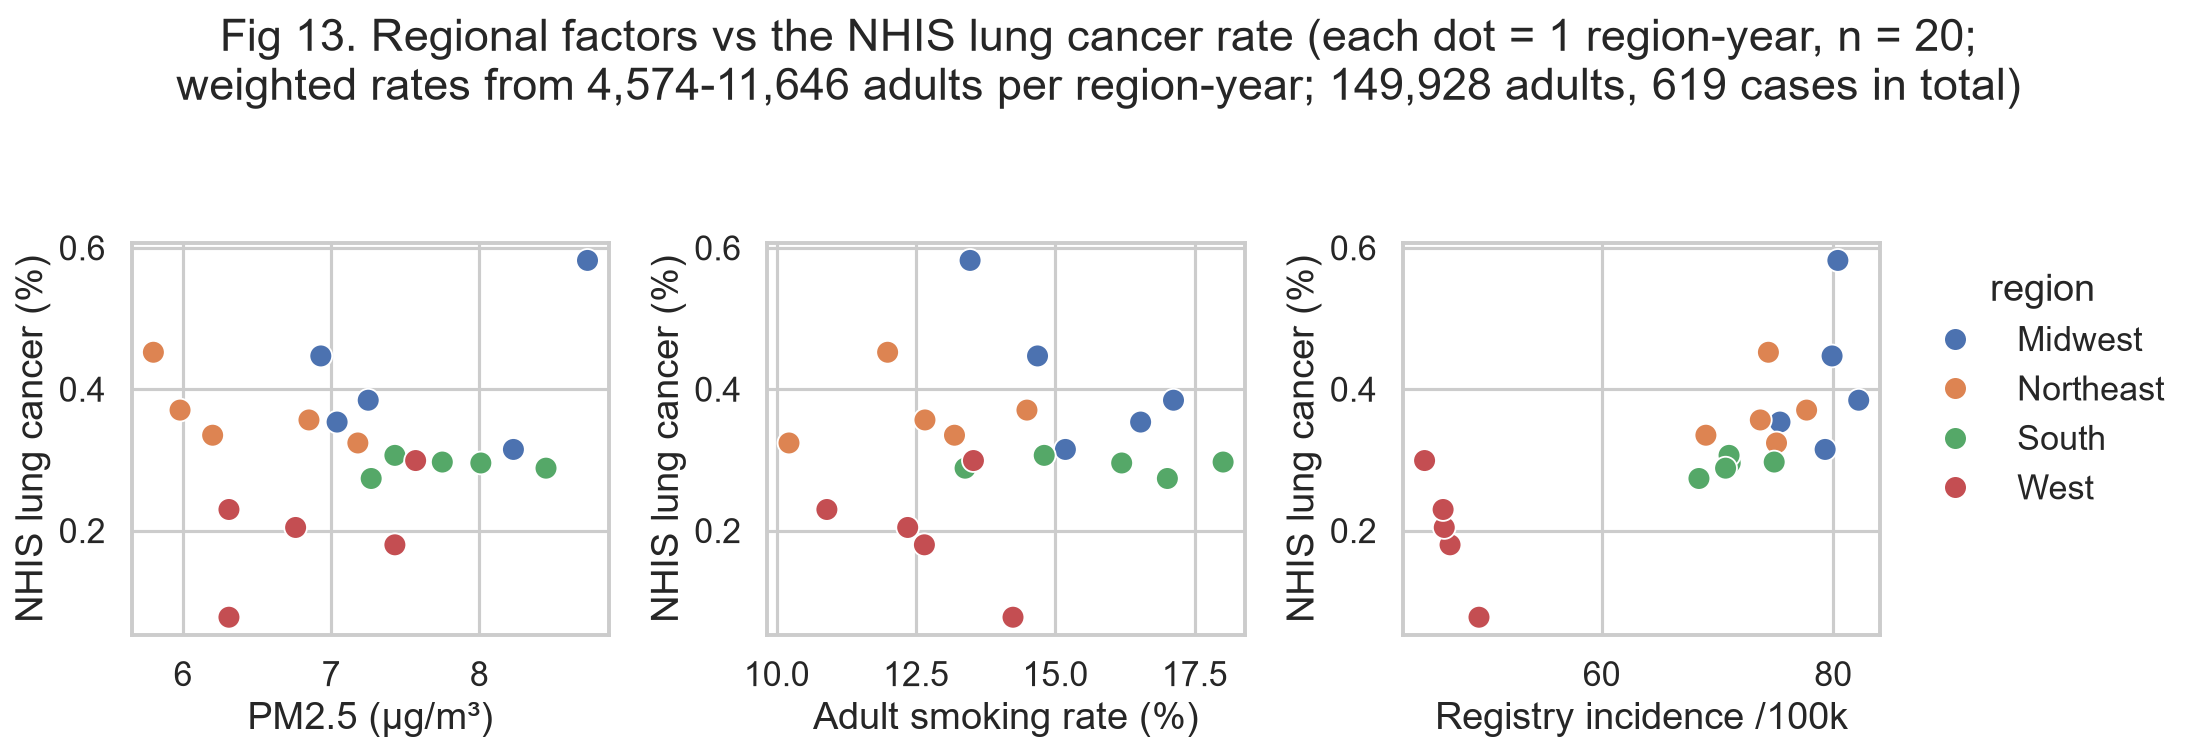
\includegraphics[width=\textwidth]{fig13_regional_factors}
\caption{Regional PM2.5, adult smoking rate and registry incidence against the weighted NHIS lung-cancer rate. Each dot is one region-year ($n$ = 20: 4 regions $\times$ 5 years); each region-year rate is the survey-weighted rate of its adults (\regionYearMin to \regionYearMax adults per region-year; \nAdults adults and \nCases cases in total).}\label{fig:regional}
\end{figure}

\begin{itemize}
  \item \textbf{The cross-source check.} Over the 20 region-years, the survey-based rate follows the official registry incidence (Fig.~\ref{fig:regional}; Spearman $\rho = \rhoRegistry$, $p$ = \pRegistry, Holm $p$ = \holmRegistry). Pooled over five years, the weighted rate is highest in the Midwest (0.42\%) and Northeast (0.37\%) and lowest in the West (0.20\%), the region with by far the lowest registry incidence (46.7 per 100,000 against 71--79 elsewhere).
  \item \textbf{Why we read it cautiously.} The 20 points are four regions measured five times, so they are not independent. Table~\ref{tab:regional} splits the correlation in two: the four regional means rank identically on both measures ($\rho = 1.0$, but $n = 4$), while the year-to-year changes within a region do not move together ($\rho = 0.03$, $p = 0.89$). The agreement is therefore mainly ``the West is low on both measures''. It is consistent with our self-reported target behaving like the official statistic, but it is not a formal validation, and its $p$-value is optimistic. The two measures also differ in kind -- lifetime history vs new cases per year. For PM2.5 and the regional smoking rate, the between-region correlation in Table~\ref{tab:regional} is exactly 0.00. This is a real value, not a computation error: both measures rank the four regions differently from the NHIS rate, the squared rank differences add up to exactly 10, and $\rho = 1 - 6 \times 10 / (4 \times 15) = 0$. With only four points, $\rho$ can take just a few values ($0, \pm 0.2, \pm 0.4, \ldots, \pm 1$), so this zero says nothing either way.
  \item \textbf{Air pollution and regional smoking rates show no association} (PM2.5: $\rho = -0.12$, $p = 0.63$; smoking rate: $\rho = 0.09$, $p = 0.71$), neither between nor within regions. With so few independent data points these tests are underpowered, so ``no evidence'' does not mean ``no effect''.
  \item \textbf{Why a null result is expected here.} The registry rate is crude, not age-adjusted (the West has a younger population); state values are averaged without population weights; and 2019--2023 pollution cannot explain cancers diagnosed many years earlier. Regional averages also say nothing about any individual (the ecological fallacy).
  \item \textbf{Do they add information beyond personal factors?} Mutual information on training rows (\S\ref{sec:mi}) puts all three regional columns far below the personal factors: about 0.5--0.6\% of the target's information, against 10.2\% for age. Their scores are above a shuffled-target noise level, but tiny. The three scores also measure the same thing. As discrete features, the regional values only say \emph{which region-year} a person lives in: \file{smoking_rate} and \file{lung_cancer_incidence} take a different value in each of the 20 region-years, so their mutual information is exactly that of the region-year label (0.00017 nats each), and PM2.5, where two pairs of region-years share a value, is slightly lower (0.00014). So the data cannot tell whether pollution, regional smoking or registry incidence matters; at this resolution the three columns together add one small region-year signal.
\end{itemize}

\begin{table}[htbp]
\centering\small
\caption{Spearman correlation of each regional measure with the weighted NHIS lung-cancer rate: over all 20 region-years, between the 4 regional means, and within regions (year-to-year deviations from each region's mean). Between-region values use $n = 4$, so $\rho$ can only take a few values; the 0.00 for PM2.5 and smoking rate is exact (see text). Source: \texttt{regional\_within\_between.csv}.}\label{tab:regional}
\begin{tabular}{lrrr}
\toprule
Regional measure & \makecell[b]{All 20\\{}region-years} & \makecell[b]{Between\\{}4 regions} & \makecell[b]{Within regions\\{}($n$ = 20)} \\
\midrule
PM2.5 & $-$0.12 ($p$ = 0.63) & 0.00 & 0.03 ($p$ = 0.89) \\
Regional smoking rate & 0.09 ($p$ = 0.71) & 0.00 & $-$0.35 ($p$ = 0.13) \\
Registry incidence & 0.79 ($p$ = $3.5\times10^{-5}$) & 1.00 & 0.03 ($p$ = 0.89) \\
\bottomrule
\end{tabular}

\end{table}

\subsection{All tests, with multiple-testing correction}\label{sec:alltests}

Running eighteen tests raises the chance of a false positive, so we corrected all of them together with the Holm method~\cite{holm} (Table~\ref{tab:all-tests}), which keeps the family-wise error rate at 5\% and is uniformly more powerful than Bonferroni.

\begin{table}[htbp]
\centering\small
\caption{All \nTests hypothesis tests with raw and Holm-adjusted $p$-values, labelled with the research question each one answers (\texttt{results/tables/all\_tests\_holm.csv}). $^{a}$The 20 region-years are not independent (4 regions $\times$ 5 years), so this $p$-value is optimistic; see \S\ref{sec:regional} and Table~\ref{tab:regional}.}\label{tab:all-tests}
\begin{tabularx}{\textwidth}{l >{\raggedright\arraybackslash}X r r l}
\toprule
RQ & Test & $p$ & Holm $p$ & Significant \\
\midrule
RQ1 & Smoking status ($\chi^2$) & $2.2\times10^{-115}$ & $3.1\times10^{-114}$ & yes \\
RQ2a & Age (Mann--Whitney $U$) & $3.1\times10^{-141}$ & $4.6\times10^{-140}$ & yes \\
RQ2b & COPD ($\chi^2$) & $<10^{-300}$ & $<10^{-300}$ & yes \\
RQ2b & COPD adjusted for smoking (CMH) & $1.5\times10^{-208}$ & $2.4\times10^{-207}$ & yes \\
RQ2b & Heart disease ($\chi^2$) & $5.6\times10^{-66}$ & $7.3\times10^{-65}$ & yes \\
RQ2b & Hypertension ($\chi^2$) & $1.3\times10^{-49}$ & $1.5\times10^{-48}$ & yes \\
RQ2b & Diabetes ($\chi^2$) & $6.7\times10^{-17}$ & $6.7\times10^{-16}$ & yes \\
RQ2b & Asthma ($\chi^2$) & $5.7\times10^{-4}$ & $2.9\times10^{-3}$ & yes \\
RQ2b & E-cigarette, ever ($\chi^2$) & 0.39 & 1.00 & no \\
RQ2c & Sex ($\chi^2$) & 0.16 & 0.62 & no \\
RQ2c & Race / ethnicity ($\chi^2$) & $1.6\times10^{-14}$ & $1.1\times10^{-13}$ & yes \\
RQ2c & Education ($\chi^2$) & $7.1\times10^{-24}$ & $7.8\times10^{-23}$ & yes \\
RQ2c & Income vs poverty line ($\chi^2$) & $8.3\times10^{-17}$ & $7.5\times10^{-16}$ & yes \\
RQ2c & BMI category ($\chi^2$) & $6.5\times10^{-15}$ & $5.2\times10^{-14}$ & yes \\
RQ2c & Self-rated general health ($\chi^2$) & $1.1\times10^{-248}$ & $1.8\times10^{-247}$ & yes \\
RQ3 & PM2.5 vs regional rate (Spearman, $n$ = 20) & 0.63 & 1.00 & no \\
RQ3 & Smoking rate vs regional rate (Spearman, $n$ = 20) & 0.71 & 1.00 & no \\
RQ3 & Registry incidence vs regional rate (Spearman, $n$ = 20)$^{a}$ & $3.5\times10^{-5}$ & $2.1\times10^{-4}$ & yes \\
\bottomrule
\end{tabularx}

\end{table}

\nSignificant of \nTests tests remain significant after correction (RQ1: 1 test, RQ2a: 1, RQ2b: 7, RQ2c: 6, RQ3: 3). The four that do not -- e-cigarette use, sex, PM2.5 and the regional smoking rate -- are discussed above. The COPD $\chi^2$ $p$-value is reported as ``$<10^{-300}$'' because it is below the smallest number the computer can represent ($\chi^2 \approx 1{,}950$ with 1 degree of freedom). For the CMH test we compute the $p$-value from the $\chi^2$ survival function, because the library's default returns 0 for such large statistics.

\textbf{Survey-design sensitivity.} Our tests treat respondents as independent draws, but NHIS is a stratified, clustered sample. To check how much this matters, \file{supplementary_analysis.py} reads the NHIS design variables (\file{PSTRAT}, \file{PPSU}) from the raw files and re-estimates the three key associations with survey-weighted logistic regression and confidence intervals clustered on the 3,160 sampling units (Table~\ref{tab:design}). The weighted odds ratios are somewhat larger than the unweighted ones, the interval widths change by a factor of 0.9 to 1.2, and every interval stays far from 1. The conclusions therefore do not depend on ignoring the design; a fully design-based analysis of every test remains a next step. The rates in our figures are survey-weighted.

\begin{table}[htbp]
\centering\small
\caption{Survey-design sensitivity: odds ratios from unweighted logistic regression (exact; the $2 \times 2$ tables elsewhere add 0.5 to each cell, e.g.\ 7.66 instead of 7.69 for smoking) and from survey-weighted logistic regression with confidence intervals clustered on the NHIS sampling units (year $\times$ stratum $\times$ PSU). Source: \texttt{design\_based\_odds\_ratios.csv}.}\label{tab:design}
\begin{tabular}{lrrr}
\toprule
Exposure & Adults & \makecell[b]{Unweighted OR\\{}[95\% CI]} & \makecell[b]{Weighted, clustered\\{}OR [95\% CI]} \\
\midrule
Ever smoked (vs never) & 145,975 & 7.69 [6.24, 9.48] & 9.14 [7.17, 11.65] \\
COPD (vs none) & 149,826 & 15.10 [12.87, 17.71] & 18.64 [15.43, 22.53] \\
Age, per 10 years & 149,575 & 2.03 [1.91, 2.16] & 2.15 [2.03, 2.27] \\
\bottomrule
\end{tabular}

\end{table}

\subsection{What the statistics do not show}\label{sec:notshow}

\begin{itemize}
  \item \textbf{No causes.} Every result here is an association in cross-sectional survey data. That smoking causes lung cancer is established elsewhere~\cite{uspstf,tammemagi}; our data only show a pattern consistent with it.
  \item \textbf{No individual risk.} A \orSmoking\unskip$\times$ odds ratio describes groups. It does not say how likely any one person is to develop lung cancer, and the regional results say nothing about individuals at all.
  \item \textbf{No dose--response.} Without pack-years we cannot test whether more smoking means more risk, which is the core of real screening rules.
  \item \textbf{``Not significant'' is not ``no effect''.} For e-cigarettes we ran a power check: with 23,470 ever-users, 122,606 never-users and a \sampleRate\% base rate, the test had 80\% power ($\alpha = 0.05$) to detect an odds ratio of about 1.34 or larger. So we can rule out a large effect in these data, but not a small one, and certainly not a long-term one that has not had time to appear.
  \item \textbf{Limited adjustment.} Smoking was adjusted for age, and COPD for smoking and age, by stratification. The other odds ratios are crude, so part of each one is age; a multivariable model (\S\ref{sec:next}) is needed to separate them all at once.
\end{itemize}

\section{Feature Engineering}\label{sec:fe}

We hand the modelling phase \nFeatures features (Table~\ref{tab:feature-list}), every one decided on training rows only, none of which can leak the answer, and none of which is an exact or near-exact linear combination of the others. The final tables are \file{nhis_lung_cancer_model_ready.csv} (original units) and \file{nhis_lung_cancer_model_ready_scaled.csv} (standardised), and every keep/drop decision, with its reason, is recorded in \file{final_features.csv}, so anyone can audit it.

\subsection{Features we created}\label{sec:created}

\begin{table}[htbp]
\centering\small
\caption{Engineered and joined features, with their definition and rationale.}\label{tab:engineered}
\begin{tabularx}{\textwidth}{@{}>{\raggedright\arraybackslash}p{3.9cm} >{\raggedright\arraybackslash}p{3.7cm} >{\raggedright\arraybackslash}X@{}}
\toprule
Feature & Definition & Why we built it \\
\midrule
\texttt{screening\_age\_smoker} & 1 if aged 50--80 and ever smoked & a proxy for the official USPSTF screening group; Fig.~\ref{fig:agesmoking} shows that risk piles up exactly there. Without pack-years it is only an approximation (an interaction feature built from domain knowledge) \\
\texttt{comorbidity\_count} & number of the 5 conditions (0--5) & one number for overall health burden, used in the EDA (Tables~\ref{tab:prof-conditions}--\ref{tab:cases}, Fig.~\ref{fig:numeric}, Fig.~\ref{fig:corr}); not a model feature, because it is the exact sum of the five condition flags (dropped by rule 4, \S\ref{sec:selection}) \\
\texttt{ever\_smoker} & current or former smoker & simple exposure flag, used for the odds ratio in RQ1 (dropped from the model set as redundant, \S\ref{sec:selection}) \\
\texttt{age\_group} & 18--44, 45--54, 55--64, 65--74, 75+ & used for reporting, the age $\times$ smoking table and the age-adjusted tests; exact age is kept for the model instead \\
\texttt{pm25\_mean}, \texttt{smoking\_rate}, \texttt{lung\_cancer\_incidence} & regional values joined on region + year (\S\ref{sec:integration}) & environmental and baseline-risk context for RQ3 \\
\bottomrule
\end{tabularx}
\end{table}

\subsection{Encoding and imputation}\label{sec:encoding}

\begin{itemize}
  \item \textbf{One-hot encoding} for the nominal variables (sex, race/ethnicity, region, smoking status) and for the grouped ordinal ones (education, income, general health, BMI, age group). We chose one-hot over label encoding so the model never assumes a false order or false equal spacing between categories (for example that ``Asian'' is ``greater'' than ``Black''). A complete set of dummies always adds up to 1, which makes a linear model impossible to fit, so the model-ready file drops one \textbf{reference category} per group and every other dummy is read relative to it: race/ethnicity \emph{White} (the largest group), education \emph{High school / GED}, income \emph{High} (four times the poverty line or more), BMI \emph{Healthy}, general health \emph{Excellent}, smoking status \emph{Never}; for sex (\emph{Male}) and region (\emph{West}) the reference was already dropped by the near-duplicate rule. The choice is recorded for every dummy in \file{final_features.csv}.
  \item \textbf{Unknown answers and the reference group.} \emph{Unknown} categories that survive selection (education, BMI) are kept as their own dummy. For smoking status, the small \emph{Unknown} dummy was dropped as a near-duplicate of \file{screening_age_smoker_unknown} ($r = 0.96$), so the 2.6\% of adults with an unknown smoking status now fall into the \emph{Never} reference group and are identified only by \file{screening_age_smoker_unknown}, which is therefore kept (\S\ref{sec:final}). The same happens to the 0.04\% with unknown general health (reference \emph{Excellent}).
  \item \textbf{Missing values} become an explicit Unknown category instead of being dropped or guessed.
  \item \textbf{Binary health columns} stay 0/1, with missing values set to 0 plus an \file{_unknown} flag; the flags for very rare gaps are later removed by the near-constant filter (\S\ref{sec:selection}).
  \item \textbf{Age} is filled with the training median (54 years); the \file{age_missing} flag created at the same time (0.24\% of adults) is later removed by the near-constant filter (\S\ref{sec:selection}).
\end{itemize}

\subsection{Scaling}\label{sec:scaling}

Four numeric features use completely different units: age in years, PM2.5 in \textmu g/m$^3$, smoking prevalence in \%, and incidence per 100,000. (The 0--5 comorbidity count is no longer a model feature, \S\ref{sec:selection}.) Distance-based and regularised models are sensitive to these scales, so we standardise them with a \file{StandardScaler} fitted on training rows only. Binary columns are already on a 0--1 scale, so we leave them alone and keep them interpretable.

\begin{table}[htbp]
\centering\small
\caption{Scaler parameters learned on the \nTrain training rows, and the mean of each scaled column on the test rows.}\label{tab:scaler}
\begin{tabular}{lrrr}
\toprule
Column & \makecell[b]{Training\\{}mean} & \makecell[b]{Training\\{}SD} & \makecell[b]{Scaled\\{}test mean} \\
\midrule
age & 52.81 & 18.33 & $-$0.002 \\
pm25\_mean & 7.289 & 0.763 & 0.006 \\
smoking\_rate & 14.475 & 2.078 & $-$0.001 \\
lung\_cancer\_incidence & 67.31 & 12.50 & 0.019 \\
\bottomrule
\end{tabular}

\end{table}

\subsection{Feature selection}\label{sec:selection}

We went from \nCandidates candidates to \nFeatures features, applying the filter pass from the course~\cite{larose,louati} on training rows only, in this order (Table~\ref{tab:selection}):

\begin{table}[htbp]
\centering\small
\caption{Feature-selection rules and the features each rule removed (\nDropped in total). Never candidates: \texttt{person\_id} (identifier), \texttt{split} (train/test label), \texttt{survey\_weight} (a sampling weight, not a property of the person) and \texttt{CANEV\_A} (reveals the answer). \texttt{sex\_Male} and \texttt{region\_West}, dropped by rule 3, also serve as the reference categories of sex and region.}\label{tab:selection}
\begin{tabularx}{\textwidth}{>{\raggedright\arraybackslash}p{5.2cm} r >{\raggedright\arraybackslash}X}
\toprule
Rule & Dropped & Features \\
\midrule
1. Redundant by construction & 8 & ever\_smoker, ever\_smoker\_unknown, age\_group\_18-44, age\_group\_45-54, age\_group\_55-64, age\_group\_65-74, age\_group\_75+, age\_group\_Unknown \\
2. Constant in training rows & 0 & -- \\
2b. Near-constant: more than 99.5\% of training rows share one value & 8 & age\_missing, copd\_unknown, asthma\_unknown, hypertension\_unknown, heart\_disease\_unknown, diabetes\_unknown, sex\_Unknown, general\_health\_Unknown \\
3. Near-duplicates: $|r| > 0.95$ with a column already kept & 3 & sex\_Male, region\_West, smoking\_status\_Unknown \\
4a. Exact linear combination of other features (VIF = $\infty$) & 1 & comorbidity\_count \\
4b. Reference category of each one-hot group & 6 & race\_ethnicity\_White, education\_High school / GED, income\_group\_High, general\_health\_Excellent, bmi\_category\_Healthy, smoking\_status\_Never \\
4c. Near-collinear block (region dummies vs regional columns) & 3 & region\_Midwest, region\_Northeast, region\_South \\
\midrule
Total dropped & 29 & 38 features kept \\
\bottomrule
\end{tabularx}

\end{table}

The near-constant rule removes columns that describe fewer than 1 adult in 200 (for example, ``COPD answer unknown'' applies to 0.06\% of adults). Such columns add almost no information but add dimensions -- the curse of dimensionality discussed in the course. We deliberately did not use target-based filtering to drop weak features: with a \sampleRate\% outcome, univariate relevance is unstable, and interactions (such as age $\times$ smoking) can make individually weak features useful. Relevance is instead checked in \S\ref{sec:mi} and will be tested by ablation in the modelling phase.

\textbf{Rule 4: dependencies spread over several columns (VIF).} Rules 1--3 compare columns one pair at a time, so they cannot see a column that is a combination of \emph{several} others. The variance inflation factor can: $\mathrm{VIF}_j = 1 / (1 - R^2_j)$, where $R^2_j$ comes from regressing feature $j$ on all the other features (with an intercept) on the training rows. $\mathrm{VIF} = 1$ means feature $j$ is unrelated to the others, $\mathrm{VIF} > 10$ is the usual alarm level, and $\mathrm{VIF} = \infty$ means an exact linear dependency. After rules 1--3, \nInfVIF of the \nFeaturesBefore features had an infinite VIF and \nVIFaboveTenBefore a VIF above 10 (Table~\ref{tab:vif}; \file{results/tables/vif_before.csv}). The causes were the comorbidity count (the sum of five flags) and the four complete one-hot groups (race, education, income, BMI), each of which summed to 1. General health and smoking status almost did (VIF 100--643, because only their small Unknown dummies had been removed), and the region dummies almost determined the registry incidence (VIF 24--39). Rule 4 removes these dependencies (\file{comorbidity_count}, one reference category per group, the three region dummies). After it, the largest VIF is \maxVIFshort, nothing exceeds 10, and the PCA has no near-zero component left (\S\ref{sec:pca}; \file{vif_after.csv}). The two features closest to the limit are \file{screening_age_smoker_unknown} (7.49) and \file{ever_ecigarette_unknown} (7.45). They overlap because both flag the adults who skipped the smoking questions, and they are kept because the first is the only marker of an unknown smoking status. The \file{screening_age_smoker} flag, built from age and smoking, has a VIF of only 2.2. None of these drops removes information: an exact dependency is a direction with zero variance, and the region dummies added almost nothing beyond the 20 region-year values of the regional columns.

\begin{table}[htbp]
\centering\small
\caption{Variance inflation factor of every feature after rules 1--3 (\nFeaturesBefore features) and after rule 4 (\nFeatures features), on training rows; one-hot groups are summarised by their range. $\infty$ = exact linear dependency.}\label{tab:vif}
\begin{tabularx}{\textwidth}{>{\raggedright\arraybackslash}p{5.5cm} r >{\raggedright\arraybackslash}X}
\toprule
Feature & VIF after rules 1--3 & VIF after rule 4 \\
\midrule
asthma & $\infty$ & 1.06 \\
bmi\_category\_* (5 dummies) & $\infty$ & 1.04--1.59 (Healthy dropped, 4b) \\
comorbidity\_count & $\infty$ & dropped (4a) \\
copd & $\infty$ & 1.18 \\
diabetes & $\infty$ & 1.17 \\
education\_* (6 dummies) & $\infty$ & 1.02--1.67 (High school / GED dropped, 4b) \\
heart\_disease & $\infty$ & 1.14 \\
hypertension & $\infty$ & 1.41 \\
income\_group\_* (4 dummies) & $\infty$ & 1.32--1.42 (High dropped, 4b) \\
race\_ethnicity\_* (7 dummies) & $\infty$ & 1.01--1.24 (White dropped, 4b) \\
age & 1.70 & 1.70 \\
ever\_ecigarette & 1.32 & 1.32 \\
ever\_ecigarette\_unknown & 15.86 & 7.45 \\
general\_health\_* (5 dummies) & 100.85--643.10 & 1.34--1.91 (Excellent dropped, 4b) \\
lung\_cancer\_incidence & 33.61 & 1.38 \\
pm25\_mean & 2.44 & 1.14 \\
region\_* (3 dummies) & 23.98--39.02 & dropped (Midwest, South, Northeast dropped, 4c) \\
screening\_age\_smoker & 2.18 & 2.18 \\
screening\_age\_smoker\_unknown & 13.11 & 7.49 \\
sex\_Female & 1.07 & 1.07 \\
smoking\_rate & 2.74 & 1.34 \\
smoking\_status\_* (3 dummies) & 113.44--258.91 & 1.72--2.03 (Never dropped, 4b) \\
\midrule
\textbf{Maximum (finite)} & 643.10 & \textbf{7.49} \\
\bottomrule
\end{tabularx}

\end{table}

\subsection{Relevance check with mutual information}\label{sec:mi}

Mutual information (MI) measures how much knowing a feature reduces uncertainty about the target, including non-linear relationships. We computed it on training rows only and treated every column with 25 or fewer distinct values as discrete; only age is treated as continuous. This matters: the continuous (nearest-neighbour) estimator is biased upwards on heavily tied values, and an earlier version of the analysis that treated the regional columns (20 distinct values each) as continuous inflated their score about tenfold (0.0016--0.0022 instead of 0.00014--0.00017), placing them wrongly in places 4--6.

With the correct estimator, the ranking agrees with the EDA: age (\miAge) and COPD (\miCOPD) lead, followed by the screening-age-smoker flag (\miScreening), poor self-rated health, former smoking and hypertension (Fig.~\ref{fig:mi}; \nTrain training rows, \nTrainCases cases). The raw values look small, but MI is bounded by the uncertainty of the target, which is tiny for a \sampleRate\% outcome (an entropy of 0.0268 nats). Expressed as a share of that maximum, age carries 10.2\% of the available information and COPD 9.8\%, against 0.5--0.6\% for each regional column (Table~\ref{tab:mi}). To check that these scores are not noise, we shuffled the target 100 times and recomputed MI: every listed feature scores above the 95th percentile of its shuffled scores, but the regional columns only just -- their real information is a small fraction of the personal factors'. The three regional columns now occupy the last three places of the top 15 (Fig.~\ref{fig:mi}). Their MI values did not change; they moved up only because ten features left the set. \file{smoking_rate} and \file{lung_cancer_incidence} have \emph{identical} scores and null percentiles, and PM2.5 is slightly lower, for a structural reason. As discrete features, the regional columns only label the region-year a person lives in: the first two take a different value in each of the 20 region-years, so both equal the mutual information of the region-year label itself (0.000173 nats). PM2.5 has two ties (6.31 \textmu g/m$^3$ in the West in 2019 and 2023; 7.43 in the South in 2022 and the West in 2021), so it merges two pairs of region-years and scores slightly less (0.000145; \file{regional_mi_identity.csv}). The three regional scores therefore measure one thing, not three independent signals, which is consistent with RQ3.

(Note on the earlier ranking: the tie between \file{screening_age_smoker} and \file{smoking_status_Never} at 0.00158 in the previous version of this table was a coincidence of rounding, not a duplicate. The two $2 \times 2$ tables differ -- the screening flag marks 25,794 training adults with 307 cases, never-smoking 72,861 adults with 90 cases -- and their MI values only differ in the eighth decimal: 0.00158140 vs 0.00158137 nats, $3 \times 10^{-8}$ apart.)

\begin{table}[htbp]
\centering\small
\caption{Mutual information on training rows, as a share of the target's entropy (0.0268 nats), against a permutation null (target shuffled 100 times; the smallest possible $p$ is $1/101 \approx 0.01$). Source: \texttt{mutual\_information\_checked.csv}.}\label{tab:mi}
\begin{tabular}{lrrrr}
\toprule
Feature & MI (nats) & \makecell[b]{Share of target\\{}entropy} & \makecell[b]{Null, 95th\\{}percentile} & \makecell[b]{Permutation\\{}$p$} \\
\midrule
age & 0.00274 & 10.2\% & 0.00080 & 0.01 \\
copd & 0.00263 & 9.8\% & 0.00002 & 0.01 \\
screening\_age\_smoker & 0.00158 & 5.9\% & 0.00001 & 0.01 \\
smoking\_status\_Former & 0.00109 & 4.1\% & 0.00001 & 0.01 \\
hypertension & 0.00072 & 2.7\% & 0.00002 & 0.01 \\
smoking\_rate & 0.00017 & 0.6\% & 0.00013 & 0.01 \\
lung\_cancer\_incidence & 0.00017 & 0.6\% & 0.00013 & 0.01 \\
pm25\_mean & 0.00014 & 0.5\% & 0.00012 & 0.02 \\
\bottomrule
\end{tabular}

\end{table}

\begin{figure}[htbp]
\centering
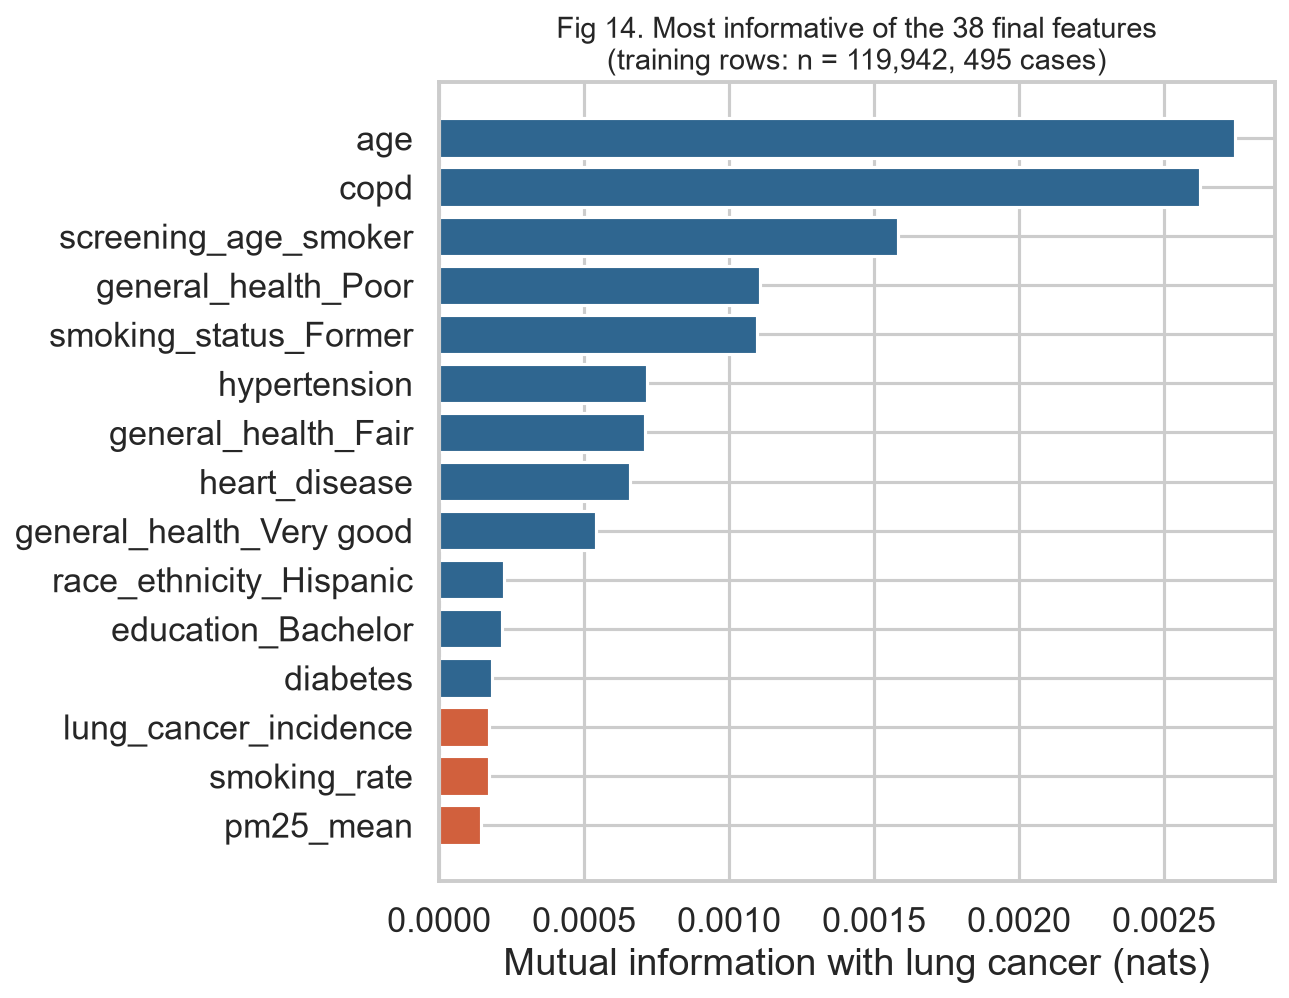
\includegraphics[width=0.65\textwidth]{fig14_feature_relevance}
\caption{Mutual information between each of the \nFeatures final features and the target on the training rows (top 15; $n$ = \nTrain adults, \nTrainCases cases). The three regional columns (orange) take the last three places; their nearly equal values reflect one shared region-year signal (\S\ref{sec:mi}).}\label{fig:mi}
\end{figure}

\subsection{Feature extraction with PCA}\label{sec:pca}

Feature selection keeps a subset of the original columns; feature extraction builds new ones. We tested whether Principal Component Analysis could compress the \nFeatures selected features without losing much information (Fig.~\ref{fig:scree}). Because the features have different units, we standardised all of them first -- equivalent to running PCA on the correlation matrix, as the course recommends~\cite{jolliffe,louati} -- and fitted both the scaler and the PCA on training rows only. Loadings are correlations between a feature and a component; only loadings with an absolute value of at least 0.40, the threshold used in the course, are listed in Table~\ref{tab:pca}.

\begin{figure}[htbp]
\centering
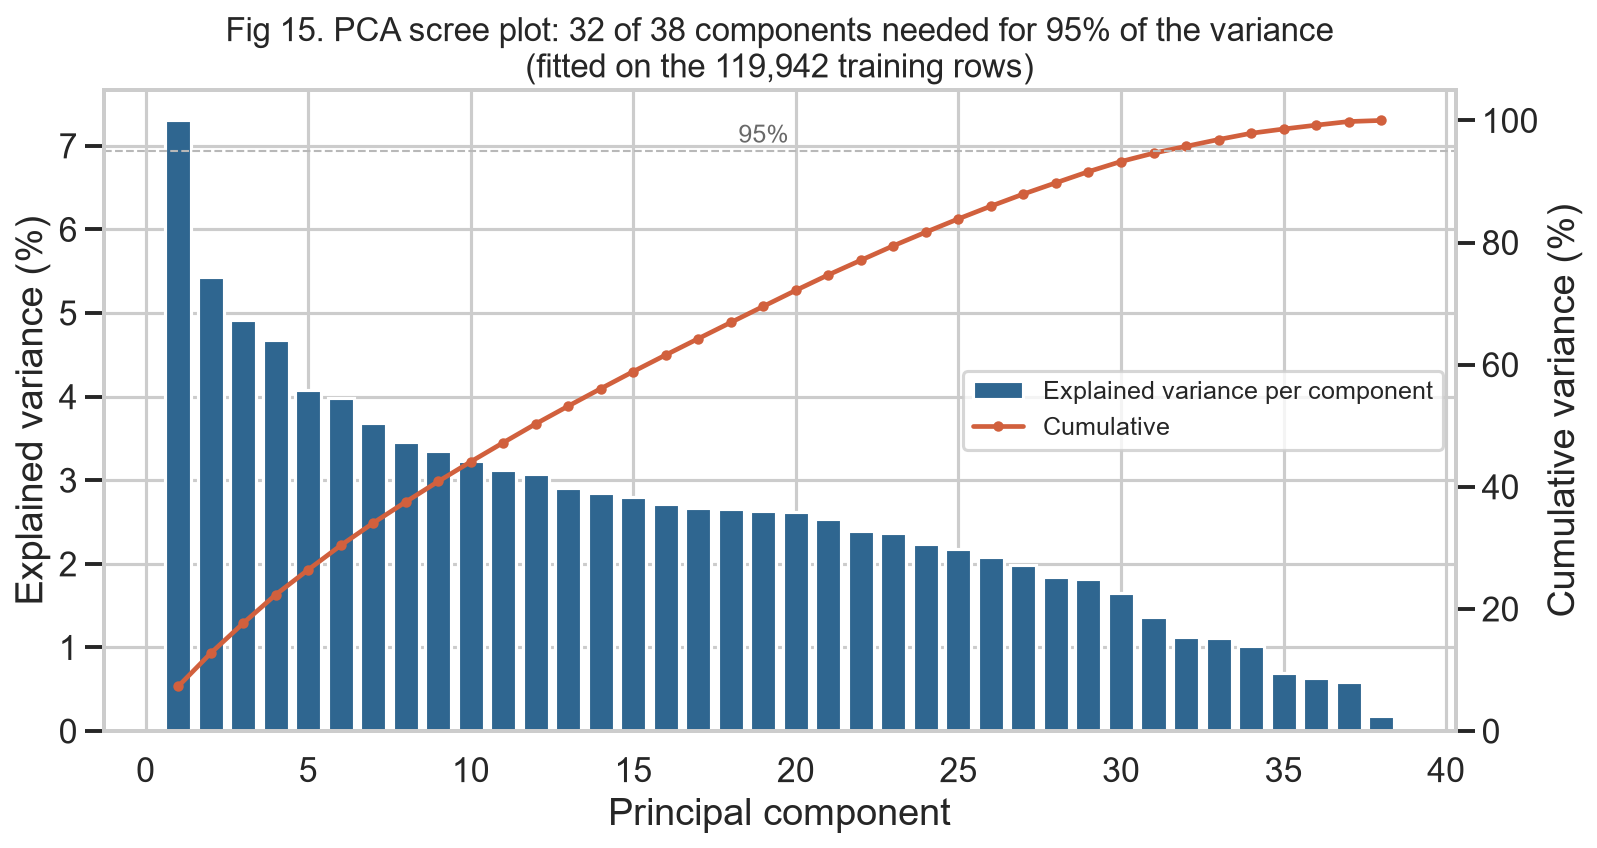
\includegraphics[width=0.8\textwidth]{fig15_pca_scree}
\caption{PCA scree plot (fitted on the \nTrain training rows): explained variance per component (bars) and cumulative variance (line). \pcaNinetyFive of \nFeatures components are needed to keep 95\% of the variance.}\label{fig:scree}
\end{figure}

\begin{table}[htbp]
\centering\small
\caption{PCA summary (fitted on the \nTrain training rows).}\label{tab:pca}
\begin{tabularx}{\textwidth}{>{\raggedright\arraybackslash}p{5.2cm} >{\raggedright\arraybackslash}X}
\toprule
Quantity & Value \\
\midrule
Variance explained by PC1 / PC2 / PC3 & 7.3\% / 5.4\% / 4.9\% (2.6\% expected per component if all features were unrelated) \\
Components needed for 80\% / 90\% / 95\% of the variance & 24 / 29 / 32 of 38 \\
Kaiser rule (eigenvalue $>$ 1) & 19 components \\
Components with almost zero variance (eigenvalue $<$ 0.01) & 0 (there were 8 with the previous 48 features: the dependencies removed by rule 4, \S\ref{sec:selection}) \\
Variance of the test rows kept by the first 32 components & 95.8\% (the PCA generalises; it never saw the test rows) \\
PC1 -- ``age and chronic-disease burden'' & hypertension +0.59, screening\_age\_smoker +0.57, age +0.57, diabetes +0.46, copd +0.45, heart\_disease +0.42 \\
PC2 -- ``skipped the smoking questions'' & screening\_age\_smoker\_unknown +0.86, ever\_ecigarette\_unknown +0.86 \\
PC3 -- ``older age vs current smoking and regional smoking level'' (mixed) & age +0.50, smoking\_rate $-$0.42 (next below 0.40: smoking\_status\_Current $-$0.39, ever\_ecigarette $-$0.38, lung\_cancer\_incidence $-$0.36, pm25\_mean $-$0.35) \\
\bottomrule
\end{tabularx}

\end{table}

\begin{figure}[htbp]
\centering
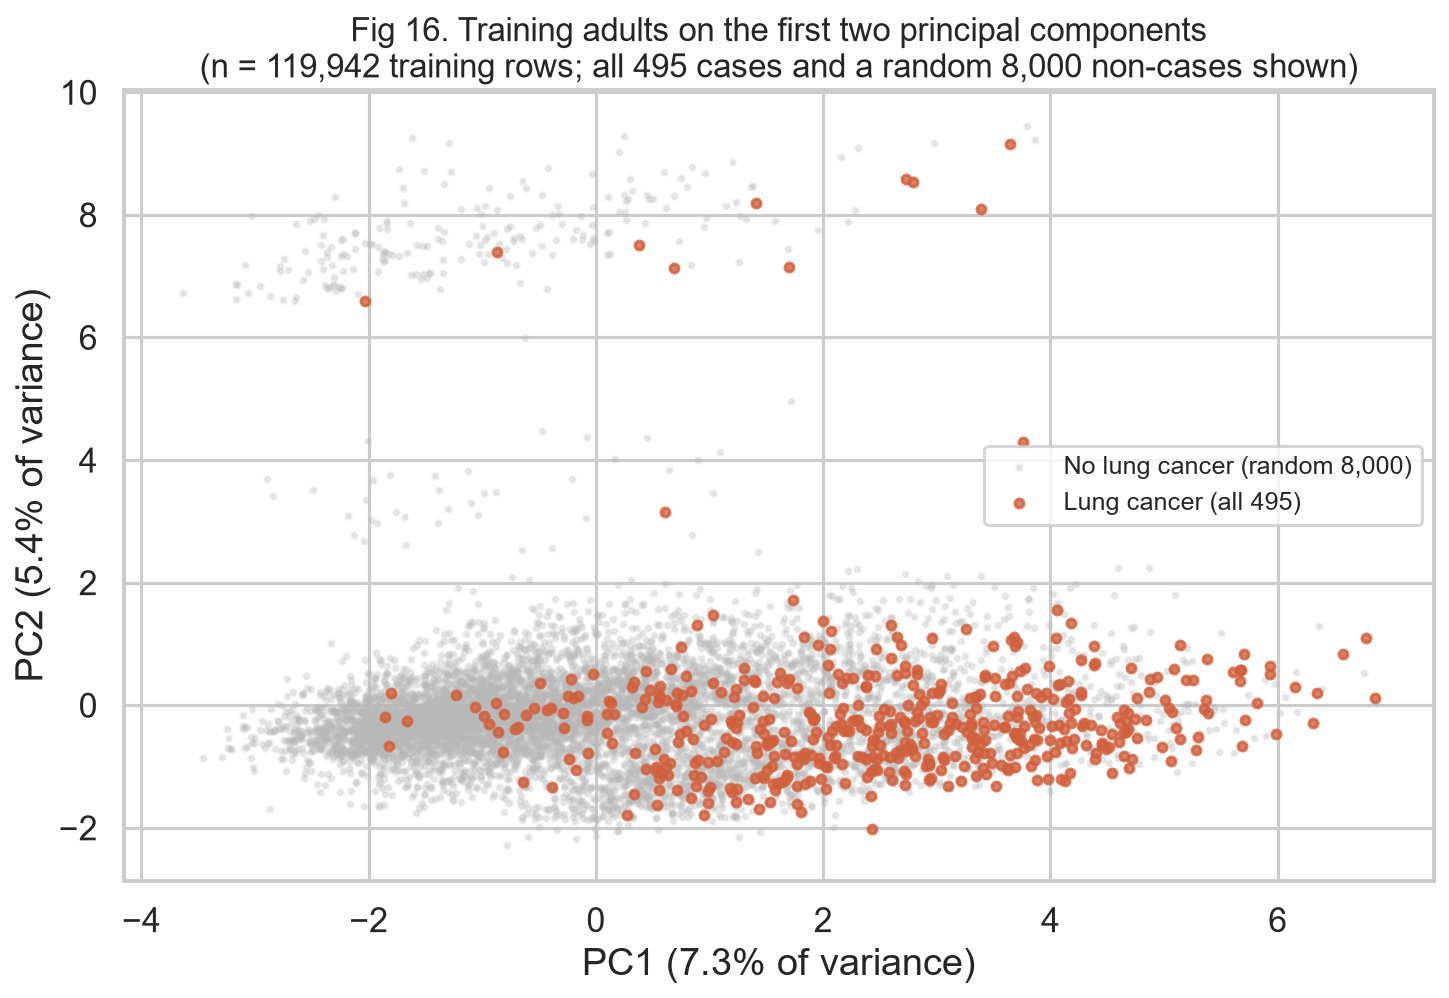
\includegraphics[width=0.75\textwidth]{fig16_pca_projection}
\caption{Training adults ($n$ = \nTrain) projected on the first two principal components: all \nTrainCases training cases (orange) and a random 8,000 non-cases (grey). The separate cloud at the top (high PC2) is the $\sim$2.8\% of adults who skipped the smoking questions.}\label{fig:projection}
\end{figure}

Lung-cancer cases sit on the high side of PC1 (Fig.~\ref{fig:projection}; mean score \pcaCaseMean vs $-0.01$ for other adults), which is the age-and-disease axis, but the two groups overlap heavily: two components cannot separate a rare outcome.

\textbf{Decision: we keep the original features.} Keeping 95\% of the variance would still need \pcaNinetyFive components -- only \pcaReduction\% fewer columns -- because the information is spread over many dimensions with no dominant one, which agrees with the weak correlations of Fig.~\ref{fig:featcorr} and the low VIFs of Table~\ref{tab:vif}. Interpretability also matters for a health question: an odds ratio for ``COPD'' means something to a clinician, a weight on ``PC4'' does not. Finally, most of our columns are 0/1 indicators, for which PCA, built for continuous data, is less natural (a method for mixed data, such as factor analysis of mixed data, would be the better tool if extraction were needed). The PCA is kept as an option to compare in the modelling phase, especially for distance-based methods such as $k$-nearest neighbours or clustering, which suffer most from many dimensions. The previous version of the feature set had eight near-zero directions. They are gone because rule 4 removed the dependencies behind them (the comorbidity count, one reference category per one-hot group, the region dummies), and that is also why the count of components dropped: an exact dependency is a zero-variance direction that carries no information.

\subsection{The final feature set and how it serves the objectives}\label{sec:final}

The \nFeatures final features are listed by group, with the reference category of every one-hot group, in Table~\ref{tab:comp-groups} (Section~\ref{sec:data}; full list in Appendix~\ref{app:features}).

\begin{itemize}
  \item It carries what the EDA found to matter -- age, smoking, COPD and the other chronic conditions (whose sum, \file{comorbidity_count}, stays in the clean dataset for the EDA only) -- in model-ready form, with no missing values and no exact or near-exact multicollinearity (maximum VIF \maxVIFshort).
  \item It links the dataset to the real clinical rule through \file{screening_age_smoker}, the baseline any future model must beat (Table~\ref{tab:screening}).
  \item It is leakage-free by construction and by check: every learned step saw training rows only, so the test score of a future model will be an honest estimate.
  \item It keeps the regional context for an ablation test rather than discarding it on the basis of four regions.
\end{itemize}

\textbf{Features we are cautious about.} \file{general_health}, BMI, current smoking status and the ``ever told'' conditions may partly be consequences of a cancer diagnosis (\S\ref{sec:sociodemo}). A model leaning on them would mostly recognise people who are already sick rather than give an early risk indication. We keep them, but plan to compare models with and without them. Race/ethnicity is kept to describe the population and to allow a fairness audit of any future model, not because race is a cause of lung cancer.

\textbf{Reading the dummies.} Every dummy is read against its group's reference category (Table~\ref{tab:comp-groups}). For smoking, the reference group \emph{Never} also contains the 2.6\% of adults whose smoking status is unknown. Their own dummy was dropped as a near-duplicate of \file{screening_age_smoker_unknown} ($r = 0.96$, rule 3), so that flag is the \textbf{only} feature that tells a model these adults are not known never-smokers. It must stay in any model that uses the smoking dummies, and an adjusted odds ratio for \emph{Current} or \emph{Former} smoking should be described as ``vs never or unknown, holding the unknown flag fixed''.

\section{Discussion}\label{sec:discussion}

\subsection{Answers to the research questions}\label{sec:answers}

Table~\ref{tab:answers} answers the five research questions with the main numbers from Sections~\ref{sec:profile} and~\ref{sec:eda}.

\begin{table}[htbp]
\centering\small
\caption{What we found for each research question.}\label{tab:answers}
\begin{tabularx}{\textwidth}{@{}>{\raggedright\arraybackslash}p{3.3cm} >{\raggedright\arraybackslash}X@{}}
\toprule
RQ & Answer \\
\midrule
RQ1 -- Smoking & Strong association. Ever-smokers have \orSmoking times the odds of never-smokers (95\% CI \orSmokingLo--\orSmokingHi), and \orSmokingMH times (4.7--7.1) after adjusting for age group; the weighted rate is 0.08\% for never-smokers vs 0.81\% for former and 0.60\% for current smokers. Former smokers ranking above current ones reflects quitting after diagnosis (reverse causation) and age, not a protective effect of smoking. \\
\addlinespace
RQ2a -- Age & Median 72 vs 54 years, rank-biserial $r = 0.59$ (a random case is older than a random non-case 79.5\% of the time); age and smoking act together (2.15--2.37\% of ever-smokers aged 75+ vs 0.48\% of never-smokers the same age). \\
\addlinespace
RQ2b -- Chronic conditions and e-cigarettes & COPD is the strongest association (odds ratio \orCOPD; among adults with known smoking status the crude \orCOPDcrude falls to \orCOPDsmoking after adjusting for smoking, consistently across smoking groups, and among those whose age is also known to \orCOPDsmokingAge after adjusting for smoking and age group); heart disease, hypertension and diabetes are moderate (2.3--4.6), partly through age; asthma is negligible; e-cigarette use shows nothing. \\
\addlinespace
RQ2c -- Socio-demographic and health factors & A clear education and income gradient, partly explained by smoking; the highest rates in underweight adults and those in poor health, most likely reverse causation; no difference by sex; race/ethnicity differences that largely follow age and smoking profiles. \\
\addlinespace
RQ3 -- Regional factors & The survey rate agrees with the official registry incidence across regions ($\rho = \rhoRegistry$ over 20 region-years, $p$ = \pRegistry), but the agreement comes from the four regional averages (mainly the low West), not from year-to-year changes within regions ($\rho = 0.03$): consistent with a valid target, not proof of it. PM2.5 and regional smoking rates show no detectable association. Regional features carry far less information than personal ones (0.5--0.6\% vs 10.2\% of the target's information for age), and the three regional columns carry one shared region-year signal, so the data cannot separate the effect of pollution, regional smoking and registry incidence. \\
\bottomrule
\end{tabularx}
\end{table}

\subsection{Did we meet our success criteria?}\label{sec:criteriamet}

All eight criteria are met (Table~\ref{tab:criteria-met}), and all eight are verified by the code rather than by hand. The pipeline also met its reproducibility rule: on a fresh environment, \texttt{python run\_all.py} rebuilt every dataset, table and figure in about 100 seconds (including the supplementary analysis), well under the five-minute target. The honest-metrics rule carries over into the modelling plan below.

\begin{table}[htbp]
\centering\small
\caption{Success criteria (Table~\ref{tab:criteria-def}) and the evidence that each is met (\texttt{success\_criteria\_check.csv}; criterion 5 is asserted in \texttt{supplementary\_analysis.py}).}\label{tab:criteria-met}
\begin{tabularx}{\textwidth}{r >{\raggedright\arraybackslash}p{5.6cm} >{\raggedright\arraybackslash}X l}
\toprule
\# & Criterion & Observed & Met \\
\midrule
1 & No duplicate person IDs & 0 & yes \\
2 & No missing values in the model-ready file & 0 missing cells & yes \\
3 & Regional join adds no rows & 149,928 $\rightarrow$ 149,928 & yes \\
4 & Same case rate in train and test & 0.41\% vs 0.41\% & yes \\
5 & No test information in fitted steps & imputation, selection (incl.\ the VIF step), scaling and PCA fitted on training rows; scaler asserted in code & yes \\
6 & Every RQ tested, with effect sizes and Holm correction & 18 tests: RQ1 (1), RQ2a (1), RQ2b (7), RQ2c (6), RQ3 (3) & yes \\
7 & Every feature has a KEEP / DROP reason & 67 of 67 candidates & yes \\
8 & CANEV\_A never a feature & absent & yes \\
\bottomrule
\end{tabularx}

\end{table}

These criteria check that the pipeline is correct; they do not measure how good a future model will be. For that, the modelling phase inherits a concrete benchmark: the USPSTF-style rule (Table~\ref{tab:screening}).

\subsection{Limitations}\label{sec:limitations}

\begin{enumerate}
  \item \textbf{Associations, not causes.} The data are self-reported and cross-sectional, so we cannot claim causation, and reverse causation affects smoking status, BMI, general health and the ``ever told'' conditions.
  \item \textbf{No smoking dose.} NHIS has no pack-years or quit dates -- the very variables the real screening rules use -- so \file{screening_age_smoker} is only a proxy.
  \item \textbf{Survey design only partly used.} Our main tests treat respondents as independent; a weighted, cluster-robust check of the three key odds ratios (Table~\ref{tab:design}) leaves the conclusions unchanged, but the other confidence intervals are still somewhat too narrow (the rates in the figures are weighted).
  \item \textbf{Rare outcome.} \nCases cases limit subgroup analysis (some race groups had to be merged; the youngest age stratum has 13 cases) and will make model estimates unstable.
  \item \textbf{Coarse regional data.} Regional variables are ecological, with only 20 distinct values from four regions; the registry rate is crude rather than age-adjusted and states are averaged without population weights.
  \item \textbf{Lifetime target.} ``Ever told'' mixes recent and old diagnoses and misses people who have died, so long-term survivors are over-represented (survivorship bias), and current pollution cannot explain past diagnoses.
  \item \textbf{Limited adjustment.} Smoking was adjusted for age and COPD for smoking and age, by stratification; all other associations are crude, and ordered variables were tested as nominal.
  \item \textbf{Pooled years.} The 2019 questionnaire redesign and the 2020 pandemic disruption could affect comparability, although the case rate does not differ significantly between years.
\end{enumerate}

\subsection{Ethical considerations}\label{sec:ethics}

NHIS is public, de-identified data, and we never attempt to re-identify anyone; household numbers are only used to check for duplicates. Because lung cancer is rare and our features are self-reported, any future model built on this work is a research prototype. It must not be presented as a screening or diagnostic tool, and false reassurance -- telling someone they are at low risk -- would be the most harmful error. Lung-cancer risk is also unequal across income and race groups, so a model could inherit those gaps; that is why race/ethnicity is kept for a fairness audit and why the fairness check below is part of the plan, not an optional extra.

\section{Conclusion and Future Work}\label{sec:conclusion}

In US adults, a lung-cancer history concentrates in older people who have ever smoked and in people with COPD -- even after accounting for smoking and age. The detailed profile of the population shows where the \nCases cases are: three in four are aged 65 or older, four in five have ever smoked, and almost half have COPD. Regional pollution and smoking levels add little at the resolution available.

\subsection{Next steps: the modelling phase (planned, not implemented)}\label{sec:next}

\begin{enumerate}
  \item \textbf{Baselines first.} An ``always no'' model and the USPSTF-style rule (\file{screening_age_smoker}). On the test rows the rule flags 21.9\% of adults, finds 66\% of the cases, and 1.25\% of the people it flags have a lung-cancer history -- three times the base rate (Table~\ref{tab:screening}). Any real model has to beat both.
  \item \textbf{Models.} Class-weighted logistic regression on the \nFeatures features -- the reference categories are already dropped and documented, and no feature has a VIF above \maxVIFshort{} -- for interpretable adjusted odds ratios, then tree-based models such as random forest and gradient boosting. Train on the fixed 80/20 split and tune with stratified 5-fold cross-validation on training rows only.
  \item \textbf{Metrics.} Recall, precision, F1 and PR-AUC, with a threshold tuned for high recall, because missing a real case costs more than a false alarm; calibration checked on the untouched test set. No accuracy.
  \item \textbf{Ablation tests.} Retrain without the reverse-causation-prone features and without the regional features, to measure what each group really contributes; compare original features with PCA components for distance-based models.
  \item \textbf{Close the survey-design gap.} Extend the weighted, cluster-robust analysis (\file{PSTRAT}, \file{PPSU}) from the three key odds ratios to every association and to the model's evaluation.
  \item \textbf{Use more of NHIS.} The raw files contain variables we did not use: age at lung-cancer diagnosis (\file{LUNGAGETC_A}, to separate recent from old diagnoses), family history of cancer and current smoking intensity.
  \item \textbf{Fairness check.} Compare recall across sex, race/ethnicity and income groups before anyone relies on the model.
  \item \textbf{Reporting standard.} Write up the model with the TRIPOD+AI checklist~\cite{tripod} and a leakage information sheet~\cite{kapoor}.
\end{enumerate}

\begin{table}[htbp]
\centering\small
\caption{The USPSTF-style rule (\texttt{screening\_age\_smoker}: aged 50--80 and ever smoked) as a benchmark: recall = share of cases flagged; precision = share of flagged adults who are cases; lift = precision divided by the base rate. Source: \texttt{screening\_rule\_baseline.csv}.}\label{tab:screening}
\begin{tabular}{lrrrrrr}
\toprule
Rows & Adults & Flagged & \makecell[b]{Cases\\{}flagged} & Recall & Precision & Lift \\
\midrule
All adults & 149,928 & 32,373 (21.6\%) & 389 of 619 & 62.8\% & 1.20\% & 2.9 \\
Test rows & 29,986 & 6,579 (21.9\%) & 82 of 124 & 66.1\% & 1.25\% & 3.0 \\
\bottomrule
\end{tabular}

\end{table}

\begin{thebibliography}{19}
\small

\bibitem{nhis} National Center for Health Statistics. National Health Interview Survey, Sample Adult files 2019--2023. Centers for Disease Control and Prevention. \url{https://www.cdc.gov/nchs/nhis/}

\bibitem{epa} US Environmental Protection Agency. AirData: annual concentration by monitor, 2019--2023. \url{https://aqs.epa.gov/aqsweb/airdata/download_files.html}

\bibitem{brfss} CDC Behavioral Risk Factor Surveillance System. BRFSS prevalence data, current smokers, 2019--2023. \url{https://data.cdc.gov/resource/dttw-5yxu}

\bibitem{uscs} CDC and National Cancer Institute. US Cancer Statistics, incidence by area, 1999--2023. \url{https://www.cdc.gov/cancer/uscs/}

\bibitem{kaggle} Kaggle user mysarahmadbhat. Lung Cancer (survey) dataset, 309 respondents; compared through the identical public copy at github.com/Akash6181/LungCancerSurvey. The rejected file \texttt{lung\_cancer\_combined\_22457.csv} was provided at the start of the project; its original provenance is not documented. \url{https://www.kaggle.com/datasets/mysarahmadbhat/lung-cancer}

\bibitem{uspstf} US Preventive Services Task Force (2021). Screening for lung cancer: recommendation statement. \emph{JAMA}, 325(10), 962--970. doi:10.1001/jama.2021.1117

\bibitem{tammemagi} Tammem\"agi, M.\,C. et al. (2013). Selection criteria for lung-cancer screening. \emph{New England Journal of Medicine}, 368(8), 728--736. doi:10.1056/NEJMoa1211776

\bibitem{holm} Holm, S. (1979). A simple sequentially rejective multiple test procedure. \emph{Scandinavian Journal of Statistics}, 6(2), 65--70.

\bibitem{cohen} Cohen, J. (1988). \emph{Statistical Power Analysis for the Behavioral Sciences} (2nd ed.). Lawrence Erlbaum.

\bibitem{crispdm} Chapman, P. et al. (2000). \emph{CRISP-DM 1.0: Step-by-step data mining guide}. SPSS Inc.

\bibitem{kapoor} Kapoor, S. and Narayanan, A. (2023). Leakage and the reproducibility crisis in machine-learning-based science. \emph{Patterns}, 4(9), 100804. doi:10.1016/j.patter.2023.100804

\bibitem{tripod} Collins, G.\,S. et al. (2024). TRIPOD+AI statement: updated guidance for reporting clinical prediction models that use regression or machine learning methods. \emph{BMJ}, 385, e078378. doi:10.1136/bmj-2023-078378

\bibitem{scipy} Virtanen, P. et al. (2020). SciPy 1.0: fundamental algorithms for scientific computing in Python. \emph{Nature Methods}, 17, 261--272.

\bibitem{sklearn} Pedregosa, F. et al. (2011). Scikit-learn: machine learning in Python. \emph{Journal of Machine Learning Research}, 12, 2825--2830.

\bibitem{statsmodels} Seabold, S. and Perktold, J. (2010). Statsmodels: econometric and statistical modeling with Python. \emph{Proceedings of the 9th Python in Science Conference}, 92--96.

\bibitem{mantel} Mantel, N. and Haenszel, W. (1959). Statistical aspects of the analysis of data from retrospective studies of disease. \emph{Journal of the National Cancer Institute}, 22(4), 719--748.

\bibitem{larose} Larose, D.\,T. and Larose, C.\,D. (2015). \emph{Data Mining and Predictive Analytics} (2nd ed.). Wiley.

\bibitem{jolliffe} Jolliffe, I.\,T. (2002). \emph{Principal Component Analysis} (2nd ed.). Springer.

\bibitem{louati} Louati, D. (2026). CS434 Data Science, lecture slides, Chapters 1 (Foundations, CRISP-DM), 2 (Data gathering and ETL), 4 (Exploratory data analysis), 5 (Feature engineering) and 6 (Descriptive modelling); and Data Science Midterm Project -- Guidelines and Evaluation Rubric. MedTech -- Mediterranean Institute of Technology.

\end{thebibliography}


\appendix
\section{Reproducibility}\label{app:repro}

We kept the project reproducible from day one, following the rule that every number and figure comes from code, never from hand edits. Code and data are in the team repository, branch main: \url{https://github.com/ZeinebMegaadi/Lung-cancer-early-detection}

Requirements: Python 3.11, 3.12 or 3.13 and the packages listed in \file{requirements.txt} (pandas, NumPy, scikit-learn, SciPy, matplotlib, seaborn, statsmodels, and jupyter, ipykernel and nbconvert for the notebook). The commands below rebuild everything:

\begin{verbatim}
git clone https://github.com/ZeinebMegaadi/Lung-cancer-early-detection.git
cd Lung-cancer-early-detection
python -m venv .venv
.venv\Scripts\Activate.ps1       (Mac / Linux: source .venv/bin/activate)
pip install -r requirements.txt
python run_all.py
python scripts/build_report.py   (this report)
\end{verbatim}

\begin{table}[htbp]
\centering\small
\caption{The six pipeline steps run by \texttt{run\_all.py}, the notebook, and the report build.}\label{tab:pipeline-steps}
\begin{tabularx}{\textwidth}{@{}l >{\raggedright\arraybackslash}p{4.6cm} >{\raggedright\arraybackslash}X@{}}
\toprule
Step & Script & Output \\
\midrule
0 & \texttt{download\_data.py} & raw NHIS, EPA, BRFSS and USCS files in \texttt{data/raw/} (skipped when already present) \\
1 & \texttt{build\_regional\_data.py} & \texttt{data/clean/regional\_context.csv} (20 region-years) and \texttt{regional\_report.txt} \\
2 & \texttt{build\_clean\_dataset.py} & clean, model-ready and scaled datasets; data dictionary; feature decisions; VIF tables (\texttt{vif\_before.csv}, \texttt{vif\_after.csv}); outlier table; before/after summary; cleaning report; Fig.~\ref{fig:outliers} \\
3 & \texttt{eda\_analysis.py} & Figures~\ref{fig:balance}--\ref{fig:missing} and \ref{fig:numeric}--\ref{fig:mi}, including Figures~\ref{fig:assoc} and~\ref{fig:featcorr}; test, correlation and association tables in \texttt{reports/tables/}; \texttt{reports/eda\_results.txt} with every test (with its denominator) and the success-criteria check \\
4 & \texttt{feature\_extraction\_pca.py} & Figures~\ref{fig:scree}--\ref{fig:projection}; \texttt{reports/pca\_results.txt}; PCA tables \\
5 & \texttt{supplementary\_analysis.py} & dataset composition (Tables~\ref{tab:comp-years}--\ref{tab:comp-groups}), population profile (Tables~\ref{tab:prof-demo}--\ref{tab:cases}), per-year rates, age-adjusted odds ratios, regional within/between check, screening-rule baseline, mutual-information check, survey-design check and the criterion-5 assertion; \texttt{reports/supplementary\_results.txt} \\
-- & \file{notebooks/lung_cancer_project.ipynb} & the whole project section by section; every code cell calls a function of the scripts above (not run by \texttt{run\_all.py}) \\
-- & \texttt{build\_report.py} & this report's generated tables and numbers (\texttt{report/generated/}); compiles \texttt{report/main.tex} with pdflatex (run twice) (not run by \texttt{run\_all.py}) \\
\bottomrule
\end{tabularx}
\end{table}

We tested this on a fresh run: the full pipeline takes about 100 seconds, finishes without errors or warnings, and the regenerated results match the committed ones. The cleaned file \file{data/clean/nhis_lung_cancer_clean.csv} ($149{,}928 \times 26$) has the SHA-256 prefix \texttt{5daf9b80b848efe9} with Unix (LF) line endings, as stored in git; pandas on Windows writes Windows (CRLF) line endings, which give the prefix \texttt{2b25cb8142487dd4} for the same data. Every script can also be imported: its steps are functions, and \texttt{main()} runs them in order. The notebook \file{notebooks/lung_cancer_project.ipynb} uses this to walk through the six CRISP-DM sections by calling those functions, with its outputs saved. By default (\texttt{REBUILD = False}) it reuses the built files; two consecutive runs were checked to leave every output byte-identical to \texttt{run\_all.py}'s. All numbers in this report come from \file{reports/eda_results.txt}, \file{reports/pca_results.txt}, \file{reports/supplementary_results.txt}, \file{reports/tables/} and \file{data/clean/cleaning_report.txt}; the tables that hold numbers and the key numbers in the text are generated from those files by \file{scripts/build_report.py}. Figure N of this report is the file \file{reports/figures/figNN_*.png} with the same number (Figures~\ref{fig:assoc} and~\ref{fig:featcorr} are \file{fig12b_*.png} and \file{fig12c_*.png}).

\section{Final feature list}\label{app:features}

The \nFeatures features of \file{nhis_lung_cancer_model_ready.csv}, in file order. Scaled columns are standardised in \file{nhis_lung_cancer_model_ready_scaled.csv}; all other columns are 0/1 indicators. Reference categories (not in the file): race/ethnicity White, education High school / GED, income High, BMI Healthy, general health Excellent, smoking status Never (which also contains unknown smoking status, flagged by feature 3), sex Male; region is represented by features 11--13.

\begin{table}[htbp]
\centering\small
\caption{The \nFeatures final features.}\label{tab:feature-list}
\begin{tabular}{rl rl}
\toprule
\# & Feature & \# & Feature \\
\midrule
1 & age (scaled) & 20 & race\_ethnicity\_Other or multiple \\
2 & screening\_age\_smoker & 21 & education\_Bachelor \\
3 & screening\_age\_smoker\_unknown & 22 & education\_Graduate \\
4 & ever\_ecigarette & 23 & education\_Less than high school \\
5 & ever\_ecigarette\_unknown & 24 & education\_Some college \\
6 & copd & 25 & education\_Unknown \\
7 & asthma & 26 & income\_group\_Below poverty \\
8 & hypertension & 27 & income\_group\_Low \\
9 & heart\_disease & 28 & income\_group\_Middle \\
10 & diabetes & 29 & general\_health\_Fair \\
11 & pm25\_mean (scaled) & 30 & general\_health\_Good \\
12 & smoking\_rate (scaled) & 31 & general\_health\_Poor \\
13 & lung\_cancer\_incidence (scaled) & 32 & general\_health\_Very good \\
14 & sex\_Female & 33 & bmi\_category\_Obese \\
15 & race\_ethnicity\_AIAN & 34 & bmi\_category\_Overweight \\
16 & race\_ethnicity\_AIAN and other & 35 & bmi\_category\_Underweight \\
17 & race\_ethnicity\_Asian & 36 & bmi\_category\_Unknown \\
18 & race\_ethnicity\_Black & 37 & smoking\_status\_Current \\
19 & race\_ethnicity\_Hispanic & 38 & smoking\_status\_Former \\
\bottomrule
\end{tabular}

\end{table}


\end{document}
